% =============================================================================
% Global SOC Mean Transit Time --- Manuscript
% =============================================================================

\documentclass[12pt, a4paper]{article}

% --- Packages ----------------------------------------------------------------
\usepackage[utf8]{inputenc}
\usepackage[T1]{fontenc}
\usepackage{geometry}
\usepackage{setspace}
\usepackage{lineno}
\usepackage{natbib}
\usepackage{graphicx}
\usepackage{float}
\usepackage{amsmath}
\usepackage{booktabs}
\usepackage{tabularx}
\usepackage{multirow}
\usepackage{hyperref}
\usepackage{xcolor}
\usepackage{authblk}
\usepackage{caption}
\captionsetup{font=small, labelfont=bf, textfont=it}
\newcommand{\PH}[1]{\textcolor{red}{#1}}

\hypersetup{
  colorlinks=true,
  linkcolor=black,
  citecolor=blue!60!black,
  urlcolor=blue!60!black
}

% --- Page layout -------------------------------------------------------------
\geometry{margin=2.5cm}
\doublespacing
\linenumbers

% ================ OPEN QUESTION: title terminology (transit vs residence) ================
% RAISED BY: Shoji (transit time is the more defensible term for tau = Cs/input; the body
%   was standardised on "mean transit time (tau)" and an intro sentence justifies it).
% STATUS: the TITLE still reads "turnover times" (and the manuscript once said "residence
%   time"). Body uses transit time throughout. Kept as-is for now (Lorenzo's call); revisit
%   only if a reviewer flags the title/body mismatch. Options if changed: "...soil organic
%   carbon transit times" or keep "turnover" as the plain-language umbrella. NOT YET FINAL.
% ========================================================================================
\title{%
  Beyond climate: the zonality of soil organic carbon transit times
}

\author[1]{Lorenzo Menichetti}
\author[2]{Shoji Hashimoto}
\author[1]{Aleksi Lehtonen}
\author[3]{Elisa Bruni}
\author[4]{\PH{[additional authors TBD]}}

\affil[1]{Natural Resources Institute Finland (Luke), Helsinki, Finland}
\affil[2]{Forestry and Forest Products Research Institute (FFPRI), Tsukuba, Japan}
\affil[3]{Laboratoire de G\'eologie, \'Ecole Normale Sup\'erieure (CNRS UMR 8538), PSL University, Paris, France}
\affil[4]{\PH{[Affiliation 4 --- TBD]}}

\date{}

\begin{document}

\maketitle

% NOTE: temporary placement before the abstract; reformat (and add CRediT / any tooling
% disclosure) once the target journal is known. See also the section at the end.
\noindent\textbf{Author contributions.}
\begin{itemize}\setlength\itemsep{2pt}
  \item \textbf{Lorenzo Menichetti}: conceived and designed the study, carried out the analysis, and wrote the manuscript.
  \item \textbf{Shoji Hashimoto}: contributed to design choices during the work and to the revision of the manuscript.
  \item \textbf{Aleksi Lehtonen}: contributed to design choices during the work and to the revision of the manuscript.
  \item \textbf{Elisa Bruni}: contributed to design choices during the work and to the revision of the manuscript.
\end{itemize}

\begin{abstract}
Soil organic carbon (SOC) turnover is commonly modelled as a global function of
climate, with the unexplained remainder treated as noise. Yet turnover responds
to more than climate (litter quality, soil texture and mineralogy, and decomposer
biology all leave a mark). Soils themselves are organised zonally, their
forming factors varying in coherent geographic patterns. An emergent property of
the soil system (the time carbon persists) may therefore share that organisation.
Using a global compilation of mineral-soil profiles, we estimate steady-state
transit times ($\tau$) and ask how much of their variation beyond climate is
attributable, organised, and mappable. Comparing all predictor groups on the same held-out geographic regions
(spatial cross-validation), climate explains about a third
of the predictable variance in $\ln\tau$; sharing the remaining explained
variance fairly among the correlated predictor groups attributes it to edaphic
context (soil texture, mineralogy and chemistry; 33\,\%),
biological context (plant productivity and decomposer community; 22\,\%), and land use
(10\,\%), with climate at 35\,\%. The beyond-climate residual is not random but
spatially organised (Moran's $I=0.25$), led by edaphic factors with soil biology
as a distinct second axis, and the response of turnover to each driver resolves
into ecologically interpretable, biome-dependent shapes. Mapping the structure
recovers a coherent zonal pattern of turnover: a data-intensive analysis of
global turnover times
converges on the long-standing pedological insight that soils, and their emergent
properties, are zonal. Because this rests on direct observations rather than model
output, it also offers an observation-based benchmark for Earth System Models:
our estimated poleward gradient in turnover is gentler, the CMIP6 models showing a
polar-to-tropical contrast roughly three times steeper and disagreeing
among themselves by an order of magnitude. We propose the zonality of soil-carbon
turnover as an interpretative framework for global SOC turnover.
\end{abstract}

\bigskip
\noindent\textbf{Keywords:} soil organic carbon; mean transit time;
decomposition kinetics; random forest; accumulated local effects;
Earth system models

\newpage

% =============================================================================
\section{Introduction}
\label{sec:intro}
% =============================================================================

\paragraph{Soil-carbon turnover and the climate feedback.}
Soils hold roughly twice as much carbon as the atmosphere, and the rate at which it
cycles rather than the stock alone defines the global C balance and the land carbon--climate feedback.
The quantity that governs this balance is the mean transit time $\tau$, the average time a carbon atom
spends in the soil from input to loss \citep{Sierra2017,Sierra2018}. We adopt the
transit-time definition, rather than the several related and often conflated
residence- or turnover-time measures, because at steady state it is the
system-level diagnostic of how long carbon persists, and it is the quantity that a
bulk single-pool inversion of stock over input actually estimates.
Because the total global stock is so large, even
modest shifts in $\tau$ over large areas have a relevant effect on the global carbon balance. What
controls $\tau$, and how it varies geographically, impacts directly whether soils
keep buffering anthropogenic emissions or begin to amplify them. Constraining that
geographic variation observationally is an active goal: recent work exploits the
present-day spatial relationship between $\tau$ and temperature as an emergent
constraint on the warming response of soil carbon \citep{Varney2020}. Such
approaches rest on the premise that the spatial $\tau$ gradient is predominantly
thermal, a premise we examine directly with our analysis.

\paragraph{The classical paradigm: chemistry and constants.}
Since the foundational models of the 1970s--1990s
\PH{[cite: Jenkinson; Parton/CENTURY; RothC lineage]}, soil organic matter decomposition has been approximated as 
first-order: the loss rate from each pool is proportional to its mass, scaled by
temperature and moisture. The rate constant $k$, and thus $\tau=1/k$, is
treated as an intrinsic property of the substrate, therefore it is spatially invariant (on top of time invariant) once those
scalars are applied, and Earth System Models (ESMs) still largely inherit this
architecture \PH{[cite: Todd-Brown 2013; Wieder 2013]}.

\paragraph{Persistence as an ecosystem property.}
This view has been progressively revised. \citet{Schmidt2011} and subsequent work
recast SOC persistence (the time carbon remains in the soil, which $\tau$ measures)
as an ecosystem rather than molecular property, emerging from
interactions among organic matter, mineral surfaces, microbial communities, and soil
structure: organo-mineral associations stabilise carbon independently of its chemistry
\PH{[cite: Kleber 2007/2021; Lehmann \& Kleber 2015]}; carbon-use efficiency varies
with community composition \PH{[cite: Kallenbach 2016; Cotrufo MEMS]}; and mycorrhizal
pathways shape belowground carbon \PH{[cite: Averill 2014]}. Decomposition kinetics, in
this framework, are still relatively constant because the SOC decay properties emerging are converging but there also is some local intrinsic variance that is the local outcome of interacting ecological, edaphic, and biological processes.

\paragraph{A zonality of soil-carbon turnover.}
If the emergent properties of SOC decomposition arise locally, then they should carry
spatial structure, and here pedology offers more than an analogy: soils are
themselves organised zonally, the soil-forming factors varying in coherent geographic
patterns, so an emergent property of the soil system will share part of that
organisation. Under this hypothesis $\tau$ is not a universal constant scaled by
climate but carries a residual spatial signal reflecting edaphic, biological, and
land-use context that climate scalars alone do not capture.

\paragraph{Climate and soil as coupled controls.}
Climate is itself a primary soil-forming factor, so edaphic properties and climate are
not independent: they carry overlapping signals about turnover. Where soil properties
predict $\tau$ about as well as climate, that shared signal expresses the zonal
coupling pedology describes. Read this way, the zonal perspective is not competing with the climate-driven account but an alternative framing of it; one that treats
climate as one soil-forming factor among several rather than the only driver. A
practical advantage follows: because these controls co-vary spatially, a zonal
description carries their combined imprint on $\tau$ implicitly, without having to
prescribe how each one acts.

\paragraph{This study.}
We therefore take a complementary route to mechanistic modelling: rather than prescribe how
non-climate context acts (imposing a structure and assumptions on a system whose processes are
incompletely known) we ask what spatial structure the observations already carry
once climate is accounted for. Compiling a global set of mineral-soil profiles and
steady-state transit times, we explore the beyond-climate variance under spatial
cross-validation: 
1) how much belongs to which process class, attributed order-independently, among
climate, edaphic context (the soil matrix itself: texture, mineralogy and
chemistry), biological context (the living system that supplies and processes
carbon: plant productivity and the decomposer community), and land use;
2) whether it is organised or noise; 
3) where context lengthens or shortens turnover, mapped at the finest scale the
data can actually resolve; and
4) how each driver acts.
Finally, we compare this structure with that of six
Earth System Models. The beyond-climate signal, though modest, carries a coherent,
ecologically interpretable structure (edaphic-led, with soil biology a distinct
second axis) which the Earth System Models we examine render with a markedly steeper
poleward gradient, and on which they themselves disagree by an order of magnitude.

% =============================================================================
\section{Methods}
\label{sec:methods}
% =============================================================================

% -----------------------------------------------------------------------------
\subsection{Conceptual framework}
\label{sec:framework}
% -----------------------------------------------------------------------------

We define the mean transit time ($\tau$) of SOC as the average time a
carbon atom spends in the soil from entry to exit
\citep{Sierra2017,Sierra2018}. Under steady-state assumptions (constant
SOC stock and input flux) and a single homogeneous pool, $\tau$ equals
the ratio of the SOC stock to the annual carbon input flux and is the
inverse of the apparent first-order decomposition rate constant~$k$:

\begin{equation}
  \tau \;=\; \frac{\text{SOC}_\text{stock}}{C_\text{input}}
  \;=\; \frac{1}{k}
  \label{eq:mtt}
\end{equation}

\noindent
We acknowledge that for multi-pool systems, $\tau$ as computed here
represents a bulk diagnostic that aggregates pools with different
turnover rates \citep{Sierra2018}. Nevertheless, this metric is widely
used as a first-order characterisation of SOC dynamics and is directly
comparable to the transit time diagnostics computed from ESM output
\citep{Carvalhais2014,Sierra2017}.

%% [design + circularity moved to "Modelling design and the attribution problem" below]

% -----------------------------------------------------------------------------
\subsection{Soil data compilation}
\label{sec:data}
% -----------------------------------------------------------------------------

We compiled soil profile data from the OpenLandMap Open Compendium
of Soil Datasets: Soil Observations and Measurements
\citep{OpenLandMapSoilDB2025} (\texttt{sol\_chem.pnts\_horizons}), a
harmonised global collection that integrates observations from many
national and regional soil surveys and ecological databases worldwide. From the full
dataset of horizon-level records, we retained only mineral soils by
removing all records with organic carbon (OC)
$\geq$~120~g~kg$^{-1}$ (the conventional threshold separating mineral
from organic soil horizons). Records with missing OC were retained at
this stage, but because a SOC stock cannot be computed without an OC
value (Eq.~\ref{eq:soc_stock}), these profiles produce no transit-time
estimate and drop out at the mean transit time step
(Sect.~\ref{sec:mtt_calc}) and are counted among the profiles flagged
as missing in Sect.~\ref{sec:results_data}.

Horizon-level soil-property measurements (the seven variables listed below)
were standardised to a 0--20~cm depth interval by
depth-weighted averaging, applied to each profile individually rather than
stratified by pedological class. For each unique soil profile (identified by
site~ID), we computed the overlap of each recorded horizon with the
0--20~cm target interval and calculated a thickness-weighted mean for
seven soil variables: organic carbon, total nitrogen, pH~(H$_2$O), clay
content, silt content, sand content, and oven-dry bulk density.
Site-level metadata (coordinates, observation date, source database)
were carried forward as the most common value across horizons.

% -----------------------------------------------------------------------------
\subsection{Data quality control}
\label{sec:qc}
% -----------------------------------------------------------------------------

After depth standardisation, the dataset contained 381\,541 profiles from
47~source databases spanning 78\textdegree S to 78\textdegree N. We applied
a series of quality-control filters to remove records likely to introduce
systematic bias into the transit-time calculation. First, 83\,206 profiles
(21.8\,\%) reported OC~$=$~0~g\,kg$^{-1}$, which in these source
databases typically encodes missing data rather than a true measurement; these values were set
to \texttt{NA} and the affected profiles were removed when no valid OC
remained. Second, 102\,379 exact duplicates (matching coordinates and OC)
were removed (26.8\,\% of all records). Third, bulk-density values outside
the physically plausible range ($<$~0.1 or $>$~2.5~g\,cm$^{-3}$) were set
to \texttt{NA}. After filtering, 198\,382 profiles remained (52.0\,\% of
the pre-QC total). Profiles with low-precision (integer-only) coordinates
($n = 208$) and unusually high OC ($>$~100~g\,kg$^{-1}$; $n = 3\,252$)
were flagged but retained.

% -----------------------------------------------------------------------------
\subsection{Bulk density gap-filling}
\label{sec:bd}
% -----------------------------------------------------------------------------

Bulk density (BD) is required to convert OC concentration to SOC stock
but is frequently unreported. We gap-filled missing BD values using a
three-tier approach. First, a Random Forest model
(\texttt{randomForest} R~package; 200~trees) was trained on the subset
of profiles with measured BD, using terrain metrics, K\"oppen zone, land
cover fractions, SoilGrids 250\,m v2.0 soil properties \citep{Poggio2021}
(excluding BD), MODIS NPP,
WRB functional group, and MODIS burn count (the cumulative number of
times each location burned over the MODIS record) as predictors. Ten-fold
cross-validation confirmed that the RF model outperformed the SoilGrids
BD product. Second, profiles lacking measured
BD but with complete RF predictors received RF-predicted values. Third,
the remaining gaps (profiles for which one or more of the RF predictors
were themselves missing, so the trained model could not be evaluated)
were filled with the SoilGrids BD product as a fallback. Each profile
was flagged with its BD source (measured, RF, or SoilGrids).

% -----------------------------------------------------------------------------
\subsection{Mean transit time calculation}
\label{sec:mtt_calc}
% -----------------------------------------------------------------------------

SOC stock for the 0--20~cm layer was calculated as:

\begin{equation}
  \text{SOC}_\text{stock}\;[\text{g\,C\,m}^{-2}]
  \;=\; \text{OC} \;\times\; \text{BD} \;\times\; 20 \;\times\; 10
  \label{eq:soc_stock}
\end{equation}

\noindent
where OC is in g~kg$^{-1}$ (as supplied by the source compilation), BD in
g~cm$^{-3}$, and depth in cm (the value~20 in the equation refers to the thickness of the
0--20~cm layer); the factor~10 reconciles these units,
converting the product $(\text{g\,kg}^{-1})(\text{g\,cm}^{-3})(\text{cm})$
into a mass per unit area, g\,C\,m$^{-2}$.

Carbon input to soil was estimated as the belowground fraction of net
primary productivity (BNPP). Root-derived carbon is preferentially stabilised in
persistent SOC (\PH{[cite: Rasse 2005; Jackson 2017]}), so the belowground
fraction is a deliberate, conservative boundary for the input flux rather than an
oversight; sensitivity to this choice, including aboveground litter and forest
harvest, is examined in Sec.~\ref{sec:robust}.
% ============ COAUTHOR POINT + DECISION: carbon input = belowground NPP only ============
% RAISED BY: both Aleksi (x2: are branches left on site? is all BNPP really litter? is
%   aboveground litter ignored?) and Shoji (using f_BNPP as the input is unusual; the
%   main source is leaf litter). Both converge on the same critique.
% DECISION (belowground as main model, defended on principle + sensitivity, not just omission):
%   1) belowground is a deliberate conservative boundary: root-derived C is preferentially
%      stabilised in persistent SOC (Rasse 2005; Jackson 2017, ~2x aboveground), so
%      f_BNPP is a principled lower boundary for the flux, not an oversight.
%   2) it is a coefficient (convention) problem, not a data gap: aboveground (1 - f_BNPP)
%      already exists per pixel by land cover. "Add aboveground litter" = raise the
%      coefficient towards 1; "add harvest" = lower it in managed pixels. Same NPP field.
%   3) scale-invariance argument (the crisp answer): every result we rest on (block-CV
%      R^2, beyond-climate gap, Shapley shares, Moran's I) is measured on log tau and is
%      scale-invariant. A spatially-UNIFORM coefficient change only rescales the tau axis
%      (provably harmless); only the spatially-STRUCTURED part can move a relative result,
%      and because our coefficient varies BY LAND COVER it projects onto the LandUse axis
%      (already an attributed predictor -> honest, not circular).
%   4) circularity (governs what may enter the denominator): land-cover/management-
%      structured coefficients are OK; climate- or biology-structured ones are forbidden in
%      the main (they would manufacture the beyond-climate signal we exist to measure).
%   TESTED: sensitivity sweep across 3 input conventions (belowground / total NPP / total-
%   harvest) shows the relative/zonality results are invariant; only the LandUse share
%   responds (Sec.~\ref{sec:robust}, Fig.~\ref{fig:input_sensitivity}, Table~\ref{tab:input_sensitivity}).
%   STATUS: settled for now, but reviewers will re-raise. Un-bibbed coefficient
%   sources still to add: Bolinder, Saunders, Komiyama, Campioli.
% =======================================================================================

We used MODIS MOD17A3 annual NPP
\citep[2001--2020;][]{Running2015} extracted at each profile location,
applying the MODIS scale factor
($\text{NPP}_\text{true} = \text{NPP}_\text{raw} / 10$;
g~C~m$^{-2}$~yr$^{-1}$). To maintain temporal consistency with the
equilibrium assumption, only NPP values from years preceding each
site's sampling date were used. Sites sampled before the MODIS era
(pre-2001) or with fewer than three pre-sampling NPP years were
excluded from the temporal statistics.

Belowground allocation fractions (BNPP/NPP) were assigned by dominant
land cover class following \citet{Mokany2006}, \citet{Malhi2011}, and
\citet{Litton2008}: tree cover 0.35, shrubland 0.45, grassland 0.55,
cropland 0.30, built-up 0.20, bare/sparse 0.30, herbaceous wetland 0.50, mangroves 0.40, moss/lichen
0.60. Sites lacking land cover information received a global average of
0.40. Soil carbon input was then:

\begin{equation}
  C_\text{input}\;[\text{g\,C\,m}^{-2}\text{\,yr}^{-1}]
  \;=\; \text{NPP} \;\times\; f_\text{BNPP}^{(\text{lc})}
  \label{eq:c_input}
\end{equation}

\noindent
where $f_\text{BNPP}^{(\text{lc})}$ is the belowground allocation fraction
for the dominant land-cover class~lc at the site (values in
Table~\ref{tab:allocation}), and $\tau$ was computed as the ratio of SOC stock to $C_\text{input}$
(Eq.~\ref{eq:mtt}). Quality control flags were assigned: values with
$\tau < 1$~year or $> 1000$~years, or with missing, negative, or
infinite values were excluded. The upper and lower 1\% tails of the
remaining distribution were removed prior to model fitting.

% ================ COAUTHOR POINT + DECISION: forest harvest removals ================
% RAISED BY: Aleksi (managed forests export biomass off-site, so aboveground litter is
%   partly fictional there). This is the input-term critique's sub-case with the most
%   teeth, because harvest is spatially ORGANISED (managed boreal/temperate forest) and
%   overlaps the beyond-climate signal, so unlike a smooth coefficient it could in
%   principle masquerade as zonality.
% DECISION: answered with a crude land-cover harvest export on tree-dominant pixels,
%   C_input = NPP * [f_BNPP + (1-f_BNPP)(1-h)], h applied only on forest pixels, swept
%   across the literature range h = 0.2-0.6 (stem-only ~0.3 boreal / ~0.45 temperate;
%   whole-tree ~0.5-0.7). The beyond-climate gap does not fall under any h; it is if
%   anything slightly larger, and only the LandUse Shapley share moves
%   (Sec.~\ref{sec:robust}, Fig.~\ref{fig:input_sensitivity}D).
% WHY NO DEDICATED MANAGED-FOREST LAYER (Hansen/Lesiv): judged unnecessary and partly
%   unsafe. (i) The crude sweep already brackets the effect and it lands on the LandUse
%   axis (already attributed). (ii) Hansen loss is episodic (wrong for a steady-state h)
%   and is already a disturbance predictor (step 05), so building h from it would
%   manufacture that predictor's importance (circularity). Lesiv (management type, ~100 m)
%   would be independent but is a new layer + full pipeline re-run + co-author re-review;
%   only worth it if the cheap sweep had moved the numbers, which it did not.
%   STATUS: settled for now; coauthors may push for a real management layer.
% ===================================================================================

% -----------------------------------------------------------------------------
\subsection{Predictor variables}
\label{sec:predictors}
% -----------------------------------------------------------------------------

Predictor variables were organised into four groups reflecting distinct
mechanisms influencing SOC turnover (Table~\ref{tab:predictors}).

\subsubsection{Climate}

Climate variables were derived from the ERA5-Land reanalysis monthly
means \citep[2001--2020;][]{MunozSabater2021}. From the original monthly
fields of 2-m air temperature (\texttt{t2m}), soil temperature at
layers~1 (0--7~cm; \texttt{stl1}) and~2 (7--28~cm; \texttt{stl2}),
volumetric soil water at layers~1 (\texttt{swvl1}) and~2
(\texttt{swvl2}), snow cover fraction (\texttt{snowc}), and potential
evaporation (\texttt{pev}), we calculated the following annual
statistics: mean 2-m temperature, temperature seasonality (monthly
standard deviation), depth-weighted mean soil temperature for 0--20~cm
(weights 0.35 for layer~1 and 0.65 for layer~2, proportional to the
overlap with the 0--20~cm interval), depth-weighted mean soil moisture
(same weights), mean snow cover fraction, and mean potential
evaporation. Climate zone was represented by the K\"oppen-Geiger
classification of \citet{Beck2023} at 30-class granularity (numeric
codes 1--30). That classification is derived from climate normals over
the 1991--2020 reference period and supplied at ${\sim}$1~km native
resolution; we resampled it to 0.1\textdegree{} by modal aggregation,
i.e.\ assigning each coarse cell the most frequent class among the fine
cells it covers (a count of classes, not an average, since the variable
is categorical).

\subsubsection{Edaphic}
% Comment by Aleksi: exclude peatlands from the ANALYSIS (not just the maps); global peat
%   maps could be used to filter observations that might distort the interpretation.
% RESOLVED 2026-07-09 (supersedes the earlier flag-not-mask decision): peat is now fully
%   EXCLUDED, not flagged. Observations on peat in the Global Peatland Map 2.0 (both tiers;
%   6,922 profiles, ~3.5%) are dropped from the fit, and peat together with open water is
%   masked (not interpreted) on all maps. See sec:robust 'Peatlands and open water'.

Soil properties were obtained from SoilGrids 250\,m v2.0
\citep{Poggio2021}, depth-weighted to 0--20~cm: clay content, sand
content, bulk density, coarse fragment volume, pH~(H$_2$O), cation
exchange capacity, and total nitrogen. All values were converted from
SoilGrids integer encoding to standard units using published
\texttt{d\_factor} scale factors (divisor~10 for texture, pH, CEC, and
coarse fragment volume; divisor~100 for bulk density and nitrogen).
This integer-to-physical-unit conversion (dividing the stored SoilGrids
integers by the \texttt{d\_factor}s above to recover g\,kg$^{-1}$, \%,
pH units, and so on) was applied identically to the values extracted at
the training points and to the gridded layers later used for global
prediction and sensitivity analysis, so the two are on the same scale.

Terrain metrics were derived from the Copernicus GLO-30 Digital
Elevation Model \citep{CopernicusDEM2022}, aggregated to
0.1\textdegree{}: mean elevation, mean slope, northness and eastness
(sine and cosine of aspect), and terrain ruggedness, defined as the
standard deviation of elevation
computed within a moving $3 \times 3$ cell neighbourhood centred on each
pixel ($\sim$30~km across).

Soil classification was based on the SoilGrids WRB Most Probable class
\citep[250\,m;][]{Poggio2021}, aggregated to 0.1\textdegree{} by mode
and reclassified into eight mechanistically defined functional groups:
sandy/coarse (Arenosols, Podzols, Regosols), temperate agricultural
(Luvisols, Cambisols, Phaeozems, Chernozems, Kastanozems,
Albeluvisols), high-clay tropical (Acrisols, Ferralsols, Lixisols,
Plinthosols, Nitisols, Alisols, Vertisols), arid/chemical (Calcisols,
Gypsisols, Solonchaks, Solonetz, Durisols), poorly drained (Gleysols,
Histosols, Fluvisols, Stagnosols, Planosols), volcanic (Andosols),
shallow/young (Leptosols, Umbrisols), and cold/permafrost (Cryosols).
These groups were encoded as integer codes for the RF models.

\subsubsection{Land use and disturbance}

Current land cover was characterised using ESA WorldCover 2021
\citep{Zanaga2022}, downloaded via the \texttt{geodata} R~package.
Eleven class-specific fractional cover layers (trees, grassland,
shrubland, cropland, built-up, bare, snow/ice, water, wetland,
mangroves, moss/lichen) were aggregated from native ${\sim}$10~m to
0.1\textdegree{} by mean. Six of these fractions (trees, grassland,
shrubland, cropland, bare, wetland) were included as continuous
predictors.

Disturbance history was captured by two products that record when the
disturbance occurred. The timing matters because we retain only events
that predate each profile's sampling date: a fire or forest loss
occurring after the soil was sampled cannot have shaped the measured
stock, and counting it would be inconsistent with the steady-state
framing. Forest loss year was extracted from the Hansen Global Forest Change v1.10 dataset
\citep{Hansen2013}; a binary flag indicated whether loss occurred before
each site's sampling date. Fire history was derived from the MODIS
MCD64A1 burned area product \citep[2001--2020;][]{Giglio2018}, with
cumulative burn count before sampling used as a continuous predictor.

\subsubsection{Biological}

Microbial community structure was represented by three independent,
spatially explicit datasets. Global soil fungal proportion (fungal
biomass as a fraction of total microbial biomass) was obtained from
\citet{Yu2022} at ${\sim}$1~km resolution. Root colonisation rates by
arbuscular mycorrhizal (AM) and ectomycorrhizal (EcM) fungi were taken
from the global maps of \citet{Barcelo2023}, along with a derived
EcM:AM root colonisation ratio. Mycorrhizal richness and endemism
(rarity-weighted richness) for both AM and EcM fungi were sourced from
the SPUN Global Underground Atlas \citep{VanNuland2025}, together with
a derived EcM:AM richness ratio. All biological layers were aggregated
to 0.1\textdegree{} by bilinear resampling. Of these nine, six form the
default set used in every analysis reported here (fungal proportion and
the five SPUN richness/endemism/ratio variables; $\geq$96\,\% coverage):
the variance attribution, the maps, and the marginal-effect curves all
rest on this six-layer set, and it is the one carried into the final
global prediction. The three \citet{Barcelo2023} root-colonisation layers
(AM and EcM colonisation and their ratio) sharply reduce coverage (to
${\sim}$61\,\%) while adding negligible unique skill, so they enter only a
nine-layer sensitivity check (Sec.~\ref{sec:robust}) and do not contribute
to the final maps or attribution.

\subsubsection{Spatial alignment}

All raster covariates were resampled to a common 0.1\textdegree{}
($\sim$11~km) global grid in WGS84 (EPSG:4326). This resolution is set by the
coarsest global covariates, the climate layers; all other inputs (SoilGrids,
MODIS, terrain) are finer and were aggregated to it. The beyond-climate signal is
in any case a meso-scale feature (Sec.~\ref{sec:mapscale}), which this grid
resolves comfortably. Continuous variables
were resampled using bilinear interpolation; categorical variables
(K\"oppen zone, WRB class) used modal aggregation. Point-level
extraction was performed at native resolution where available and from
the 0.1\textdegree{} layers otherwise.

% -----------------------------------------------------------------------------
\subsection{Modelling design and the attribution problem}
% ---------------------------------------------------------------------------
We organise predictors into four mechanistically distinct groups (Climate,
Edaphic, Land use, and Biological; Table~\ref{tab:predictors}) and model
$\ln\tau$ with Random Forests. Productivity variables (NPP, leaf area index) are
excluded by design: because $\tau$ is computed as SOC stock divided by an
NPP-derived input (Eq.~\ref{eq:mtt}), admitting productivity as a predictor would
make the model circular.

The central analytical question is how much of the predictable variation in $\tau$
belongs to each group. The groups are spatially correlated, which is mainly because climate is itself a soil-forming factor, so
climate and edaphic descriptors carry overlapping information (Sec.~\ref{sec:intro}), and the explained variance cannot be attributed to correlated predictors by simply adding them one at a
time, since the share each predictor appears to contribute then depends on the order in which they enter. We
therefore attribute variance with an order-independent decomposition (Shapley
values, Sec.~\ref{sec:shapley}) rather than with nested increments, and we test
separately whether the variance left unexplained by climate is spatially organised
(Sec.~\ref{sec:moran}), where it acts (Sec.~\ref{sec:mapscale}), and how each
driver acts (Sec.~\ref{sec:ale}). The subsections that follow set out
each of these analyses in turn; this overview only sketches the logic that links
them, deferring the methodological detail of each analysis to its own subsection
below.

Throughout, we label nested model configurations by the groups they contain:
\textbf{M1} (Climate only), \textbf{M2} ($+$\,Edaphic), \textbf{M3} ($+$\,Land use),
\textbf{M4} ($+$\,Biological), \textbf{M5} (Climate\,$+$\,Edaphic\,$+$\,Land use;
all abiotic predictors), \textbf{M6} (Climate\,$+$\,Edaphic\,$+$\,Biological), and
\textbf{M7} (the full model, all four groups). Unless noted, every M-model uses the
six-layer biological set (fungal proportion and five SPUN richness/endemism metrics);
a nine-layer set that adds the three \citet{Barcelo2023} root-colonisation layers is
fitted only as a sensitivity (Sec.~\ref{sec:robust}).

% ---------------------------------------------------------------------------
\subsection{Random Forest fitting and spatial cross-validation}
\label{sec:rf}
% ---------------------------------------------------------------------------
All models were fitted with the \texttt{ranger} package \citep{Wright2017}
(500~trees, minimum node size~5, $m_\text{try}=\lfloor\sqrt{p}\rfloor$), on
$\ln\tau$, with predictions back-transformed by exponentiation. Predictive
performance is reported throughout as the spatially cross-validated $R^2$: the
same $R^2$ goodness-of-fit measure, but computed on whole geographic blocks held
out of training rather than on the training data itself. We call this the
\emph{spatially-honest} skill, to distinguish it from in-sample fit or
interpolation between near-coincident samples. We use the term descriptively (a skill that
does not let an almost-coincident training neighbour stand in for genuine
out-of-region prediction) and not as a verdict on other validation choices.
It was estimated by spatial block cross-validation: the globe was partitioned into
$2\textdegree\times2\textdegree$ blocks ($\sim$200~km), blocks were assigned to ten
folds, and each fold's blocks were predicted from a model trained on the other
nine. Holding out whole blocks (rather than individual points) prevents a
site near a fold boundary from being predicted by an almost-coincident training
neighbour, so the reported $R^2$ measures generalisation to unseen regions rather
than interpolation between adjacent samples.

The $2\textdegree$ block ($\sim$200~km) is far wider than the distance over
which the beyond-climate residual stays correlated (its
empirical semivariogram range is $\approx16$~km; Sec.~\ref{sec:mapscale}), so a
held-out block and its nearest training points are far enough apart to be
effectively independent (no prediction is propped up by an
almost-coincident training neighbour). The attribution
is also insensitive to the block size: although the absolute cross-validated $R^2$
declines as blocks enlarge (stricter spatial separation, fewer effective degrees
of freedom), repeating the decomposition with $1\textdegree$ and $5\textdegree$
blocks shifts each group's share of attributable
variance by at most 2 percentage points, leaving the ranking and the
climate-versus-non-climate split unchanged. (Fig.~\ref{fig:blocksize})

% ---------------------------------------------------------------------------
\subsection{Attribution of variance among process classes (Shapley)}
\label{sec:shapley}
% ---------------------------------------------------------------------------
\textit{In brief.} To say how much of the predictable variation in $\tau$ each
process class accounts for, we use a variance decomposition based on Shapley
values to attribute the model's explanatory power among correlated inputs.
The procedure is direct: we refit the model for
every possible combination of the four predictor groups and, for each group,
measure how much its inclusion raises the explained variance, averaged over all
the orders in which the groups could be added. Averaging over orders is what
makes the resulting share independent of any arbitrary sequence, the property
that nested, add-one-at-a-time increments lack when predictors are correlated.

\textit{Formally.} Let $N$ be the four groups and $v(S)$ the spatially
cross-validated $R^2$ of the Random Forest fitted on exactly the groups in the
subset $S\subseteq N$. We fit all $2^{4}=16$ subsets on a single common set of
rows (those complete across all groups, $n=154{,}675$) so that every $v(S)$ is
estimated on the same observations and the subset scores are mutually
comparable. The Shapley value of group $i$ is
\begin{equation}
  \phi_i \;=\!\! \sum_{S\subseteq N\setminus\{i\}}
  \frac{|S|!\,\bigl(|N|-|S|-1\bigr)!}{|N|!}\,
  \bigl[\,v(S\cup\{i\})-v(S)\,\bigr],
  \label{eq:shapley}
\end{equation}
the order-averaged marginal contribution of $i$; the $\phi_i$ sum exactly to the
full-model $R^2=v(N)$, and we report each as a percentage share. Alongside the
Shapley shares we report, for each group, its single-domain skill $v(\{i\})$.
The two are complementary readings of the same model set: the single-domain
skill is how well a group predicts $\tau$ \emph{on its own} (shared information
included), whereas the Shapley share is how much a group \emph{adds once the
others are present} (shared information divided evenly among the groups that
carry it). Where predictors are correlated the two can diverge, so reading them
side by side separates a group's total signal from its unique contribution; we
note below that for these data they in fact agree closely on the ranking of
groups. We also report the overlap $\sum_i v(\{i\}) - v(N)$, which quantifies
how much the groups' explanatory contributions coincide: a large overlap
signifies predictors that are correlated but not redundant, and (following the
argument of Sec.~\ref{sec:intro}) is itself an expression of the zonal coupling
between climate and soil rather than a defect of the design.

The three \citet{Barcelo2023} root-colonisation layers add negligible unique skill
($\Delta R^2\approx0.001$) while reducing biological coverage from $\geq$96\% to
61\%, and so enter only the nine-layer sensitivity (Fig.~\ref{fig:parsimony};
Sec.~\ref{sec:robust}).

% ---------------------------------------------------------------------------
\subsection{Spatial organisation of the beyond-climate residual (Moran's $I$)}
\label{sec:moran}
% ---------------------------------------------------------------------------
\textit{In brief.} Attribution says how much non-climate variance exists; it does
not say whether that variance is spatially organised or merely scattered.
We test this with Moran's $I$, which asks whether places near one another carry
more similar values than they would if the values were shuffled at random across
space. Concretely, we describe each region (a spatial block) by two numbers: its
own mean beyond-climate residual, and the average residual of the blocks
surrounding it. Plotting the second against the first, a positive relationship
means neighbouring places tend to share high or low values (spatial
organisation), and the slope of that relationship is Moran's $I$. $I\approx0$
indicates no spatial pattern; $I>0$ indicates that nearby locations resemble
each other (the signature of an organised geography). How many blocks count as
``surrounding,'' and hence the scale at which organisation is measured, is set
in the formal definition below.

\textit{Formally.} We take the beyond-climate residual as the out-of-sample
$\ln\tau$ minus the climate-only prediction, aggregate it to block means, and
compute
$I=\frac{n}{\sum_{ij}w_{ij}}\cdot
\frac{\sum_{ij}w_{ij}(x_i-\bar x)(x_j-\bar x)}{\sum_i (x_i-\bar x)^2}$,
where the spatial lag $\sum_j w_{ij}x_j$ is each block's average over its eight nearest
neighbouring blocks (a row-standardised $k$-nearest-neighbour weight, $k=8$, in any
direction, not a fixed-distance radius).
Significance is assessed against a null distribution from 999 random spatial
permutations of the residuals. We evaluate $I$ at two block aggregation
resolutions, $2\textdegree$ and $5\textdegree$ (the grid-cell size to which
residuals are averaged; the neighbour count $k=8$ is held fixed).

% ---------------------------------------------------------------------------
\subsection{Mapping the zonality, and choosing the scale}
\label{sec:mapscale}
% ---------------------------------------------------------------------------
\textit{In brief.} To show where non-climate context bends turnover, we map, at
each grid cell, the ratio of the full model's predicted $\tau$ (climate together
with edaphic, biological, and land-use context; model M7) to the climate-only
model's predicted $\tau$ (M1). This is a simple per-pixel operation between two
prediction layers; we take its logarithm so that lengthening and shortening are
symmetric, and aggregate to the mapping scale. Values above
one mark regions where edaphic or biological context lengthens turnover relative to
what climate alone implies, values below one where it shortens it. Such a map is
only worth drawing at a scale where it is reliable. Two analyses set that scale.
First, most of the point-to-point variation in the residual is unstructured: a
variogram shows roughly two-thirds of its variance is short-range noise. Second,
and more directly, we measured how faithfully the map reproduces the observed
residual as it is aggregated to coarser blocks; agreement roughly doubles from the
noisy native pixel to a meso scale and then plateaus, with no single privileged
resolution. We therefore map at $2\textdegree$, within that plateau.

\textit{Formally.} The modulation field is the log-ratio of model predictions,
$\ln[\hat\tau_{\text{context}}/\hat\tau_{\text{climate}}]$, computed symmetrically
(each domain relative to climate, with no abiotic-before-biology ordering) to match
the order-independent attribution; the abiotic and biological panels are shown
separately. From the same non-climate modulation fields we also derive a discrete
zonation (Fig.~\ref{fig:zonality}c): at each 2\textdegree{} block we weight each
domain's log-ratio modulation by its Shapley share and label the block by the
largest, or as ``climate alone'' where none exceeds a small threshold. Climate
remains the baseline of this map, as of the continuous panels, so the
classification identifies the dominant \emph{beyond-climate} modulator, not the
dominant control overall. The noise floor is characterised by an empirical variogram of the
residual (nugget/sill ratio and range). The mapping scale is set by an
out-of-sample skill curve: using spatial-block-CV predictions, we form the native
beyond-climate map $\hat r_i=\hat\tau_{\text{full}}-\hat\tau_{\text{climate}}$ and
the observed residual $r_i$, aggregate both to block means at a series of block
sizes, and report $R^2(\bar r,\hat{\bar r})$ as a function of scale. This agreement
rises from $\approx0.11$ at the native pixel to $\approx0.22$ at
1--2\textdegree{} and is flat across 1--7\textdegree; a purely linear version of the
same diagnostic instead declines with scale, so the meso-scale choice rests on the
nonlinear, map-faithful metric (Appendix).

% ---------------------------------------------------------------------------
\subsection{Mechanism: marginal responses (ALE)}
\label{sec:ale}
% ---------------------------------------------------------------------------
\textit{In brief.} Attribution and the map say how much and where; to say how
each driver acts we trace the response of $\tau$ to each predictor while letting the
other predictors keep their naturally co-occurring values. In practice we slice a
predictor's range into many narrow intervals and, within each interval, measure how
much the model's prediction changes when only that predictor moves from the lower
to the upper edge of the interval; these local differences are accumulated across
intervals to trace out the response curve (in effect a binned local gradient,
accumulated and then plotted). Working locally, within intervals of co-occurring
data, is what lets Accumulated Local Effects (ALE) avoid the extrapolation
artefacts that partial-dependence curves suffer when predictors are correlated.

\textit{Formally.} We use ALE \citep{Apley2020} on the full model (M7, six-layer biology). Each continuous predictor is split
into 40 quantile bins; within each bin the predictor of interest is moved from the
lower to the upper edge of the bin while all other predictors are held at their
observed values, and the local prediction differences are accumulated and centred. Curves are computed globally and within four latitude
bands (southern temperate, tropics, northern temperate, boreal/Arctic).
Categorical predictors (K\"oppen zone, soil functional group) are excluded.

% ---------------------------------------------------------------------------
\subsection{Comparison with Earth System Model structure}
\label{sec:esm}
% ---------------------------------------------------------------------------
We compare the spatial structure of our $\tau$ against six CMIP6 models spanning
structurally distinct land-surface lineages \citep{Varney2022}: CESM2, UKESM1-0-LL,
IPSL-CM6A-LR, MPI-ESM1-2-LR, CanESM5, MIROC-ES2L. For each we computed the
quasi-equilibrium turnover $\tau_\text{ESM}=\text{cSoil}/\text{rh}$
\citep{Koven2017,Carvalhais2014} over 1980--2014 (using \texttt{cSoilAbove1m} for
CESM2 to reduce depth mismatch).

Absolute turnover is not comparable across products: depth, pool definition, and
reference period all differ, and these differences are unavoidable in cross-ESM
$\tau$ comparison. We therefore do not treat any product as a standard of truth and
do not certify absolute skill; we compare only the normalised spatial
structure. Each product is normalised to its own distribution, and structure
is summarised two ways: relative turnover by biome zone (main text) and by
continuous latitude band (appendix), together with magnitude-free dispersion
statistics (coefficient of variation, 95:5 percentile ratio, SD of $\ln\tau$). We
quantify the latitudinal amplification as the polar-to-tropical ratio of relative
turnover in each product, and compare it with the same ratio in the map estimated
here.

% ---------------------------------------------------------------------------
\subsection{Robustness checks}
\label{sec:robust}
% ---------------------------------------------------------------------------
Five checks bound the main claims (details and figures in the Appendix).
\emph{Provenance.} To test whether the residual structure could be an artefact of
combining many source databases, we measured the between-source share of residual
variance ($\eta^2$) and the change in coarse organisation after removing each
source's mean. \emph{Biological parsimony.} We compared per-layer coverage,
collinearity, and unique skill to justify the six-layer set against the
nine-layer alternative. \emph{Block-size sensitivity.} We repeated the Shapley
decomposition at $1$, $2$, and $5\textdegree$ cross-validation blocks
(Sec.~\ref{sec:rf}) to confirm that the attributed shares, and in particular
the climate-versus-non-climate split, are a property of the data rather than
of how strictly spatial independence is enforced: enlarging the block lowers
the absolute skill but should not redistribute variance among the groups if
the attribution is robust.

\emph{Carbon-input convention.} Because the soil carbon input is set by a
coefficient on one NPP field (Eq.~\ref{eq:c_input}) rather than by independent
data, we tested whether the choice of convention alters the relative results. A
spatially uniform change in that coefficient rescales $\tau$ and leaves every
scale-invariant quantity (block-CV $R^2$, the Shapley shares, and Moran's $I$)
unchanged; only spatial variation of the coefficient, which enters through land
cover, can move the attribution. We therefore re-derived $\tau$ on the same NPP
field under three conventions (belowground, total NPP, and total minus a generous
forest-harvest export on tree-dominant pixels) and re-ran the full decomposition.
The beyond-climate gap, Moran's $I$, and the Shapley shares are essentially
unchanged (Fig.~\ref{fig:input_sensitivity}, Table~\ref{tab:input_sensitivity});
only the LandUse share responds, as expected for a land-cover-structured
coefficient, and the beyond-climate signal is if anything slightly larger under
harvest. Sweeping the harvest export fraction across its literature range (0.2 to
0.6) does not lower the gap (Fig.~\ref{fig:input_sensitivity}D).
\emph{Peatlands and open water.} The analysis is scoped to mineral soils.
Observations falling on peat in the Global Peatland Map 2.0
\citep{GreifswaldGPM2022} (both the peat-dominated and peat-in-mosaic tiers;
6,922 profiles, 3.5\%) are excluded from the fit, and peat together with open
water is masked, rather than interpreted, on all maps.
%
% ====================== OPEN QUESTION (Aleksi, 2026-07-08) =======================
% COMMENT (Aleksi): How about excluding peatlands from the ANALYSIS (not
%   necessarily the maps)? If we have observations from peatlands, those could
%   distort our interpretation. There are global peat maps we could use to filter.
% NOTE (Lorenzo): Working now on excluding it explicitly
% ================================================================================

% ---------------------------------------------------------------------------
\subsection{Software and reproducibility}
% ---------------------------------------------------------------------------
Analyses used R~($\geq4.3$) with \texttt{terra}, \texttt{sf}, \texttt{ranger}
\citep{Wright2017}, and \texttt{gstat} (variograms). The pipeline is a sequence of
numbered scripts from data assembly through prediction, attribution, organisation,
mapping-scale, sensitivity, and ESM comparison; each reported number and figure
regenerates from a named script. Code and intermediate outputs are archived at
\PH{[DOI]}.

% =============================================================================
\section{Results}
% =============================================================================

% -----------------------------------------------------------------------------
\subsection{Data compilation and quality control}
\label{sec:results_data}
% -----------------------------------------------------------------------------

The initial extraction from the compendium yielded 1\,459\,728
mineral-soil horizon records, which depth standardisation collapsed to
381\,541 unique profiles (0--20~cm). Quality-control filtering
(Sect.~\ref{sec:qc}) reduced the dataset to 198\,382 profiles drawn from
44~source databases, with USDA\_NCSS contributing the largest share
(20.4\,\%), followed by Netherlands.BIS (11.5\,\%), SISLAC (8.9\,\%),
CSIRO\_NatSoil (7.0\,\%), and AfSPDB (6.7\,\%).

Observation dates ranged from 1900 to~2024,
with the majority (79\,\%) falling between~1980 and~2020. Of the
198\,382 profiles, 38\,292 (19.3\,\%) had measured bulk density, 133\,557
(67.3\,\%) received RF-predicted values, and 21\,830 (11.0\,\%) were
gap-filled with SoilGrids. The steady-state transit-time calculation
(Sect.~\ref{sec:mtt_calc}) produced valid estimates for 185\,601 profiles
(93.6\,\%), with the remainder flagged as infinite ($n = 719$), missing
input data ($n = 9\,486$), or outside the plausible range
($<$~1~or~$>$~1\,000~yr; $n = 2\,576$). For model fitting, we removed
the 1st and 99th $\tau$ percentiles, retaining 181\,887 profiles
($\tau$ range 1.9--143.9~yr). Spatial coverage spanned
78\textdegree S--78\textdegree N and 172\textdegree W--176\textdegree E
(Fig.~\ref{fig:sampling}).

% -----------------------------------------------------------------------------
\subsection{Attribution of variance among process classes}
\label{sec:results_models}
% -----------------------------------------------------------------------------

On the common set of rows complete across all four predictor groups
($n=150{,}863$), the full model explained 39\,\% of the spatially-honest
(spatial-block cross-validated; Sec.~\ref{sec:rf}) variance in $\ln\tau$
($R^2=0.390$), against 32\,\% for
climate alone ($R^2=0.319$), a beyond-climate increment of about
7~percentage points. The order-independent Shapley decomposition
(Eq.~\ref{eq:shapley}; Fig.~\ref{fig:shapley}) attributes the full model's
explained variance in $\ln\tau$ as
Climate~35.4\,\%, Edaphic~32.7\,\%, Biological~22.2\,\%, and Land~use~9.6\,\%:
climate accounts for about one third of the attributable variance and the
non-climate classes for the remaining two thirds.

\begin{figure}[H]\centering
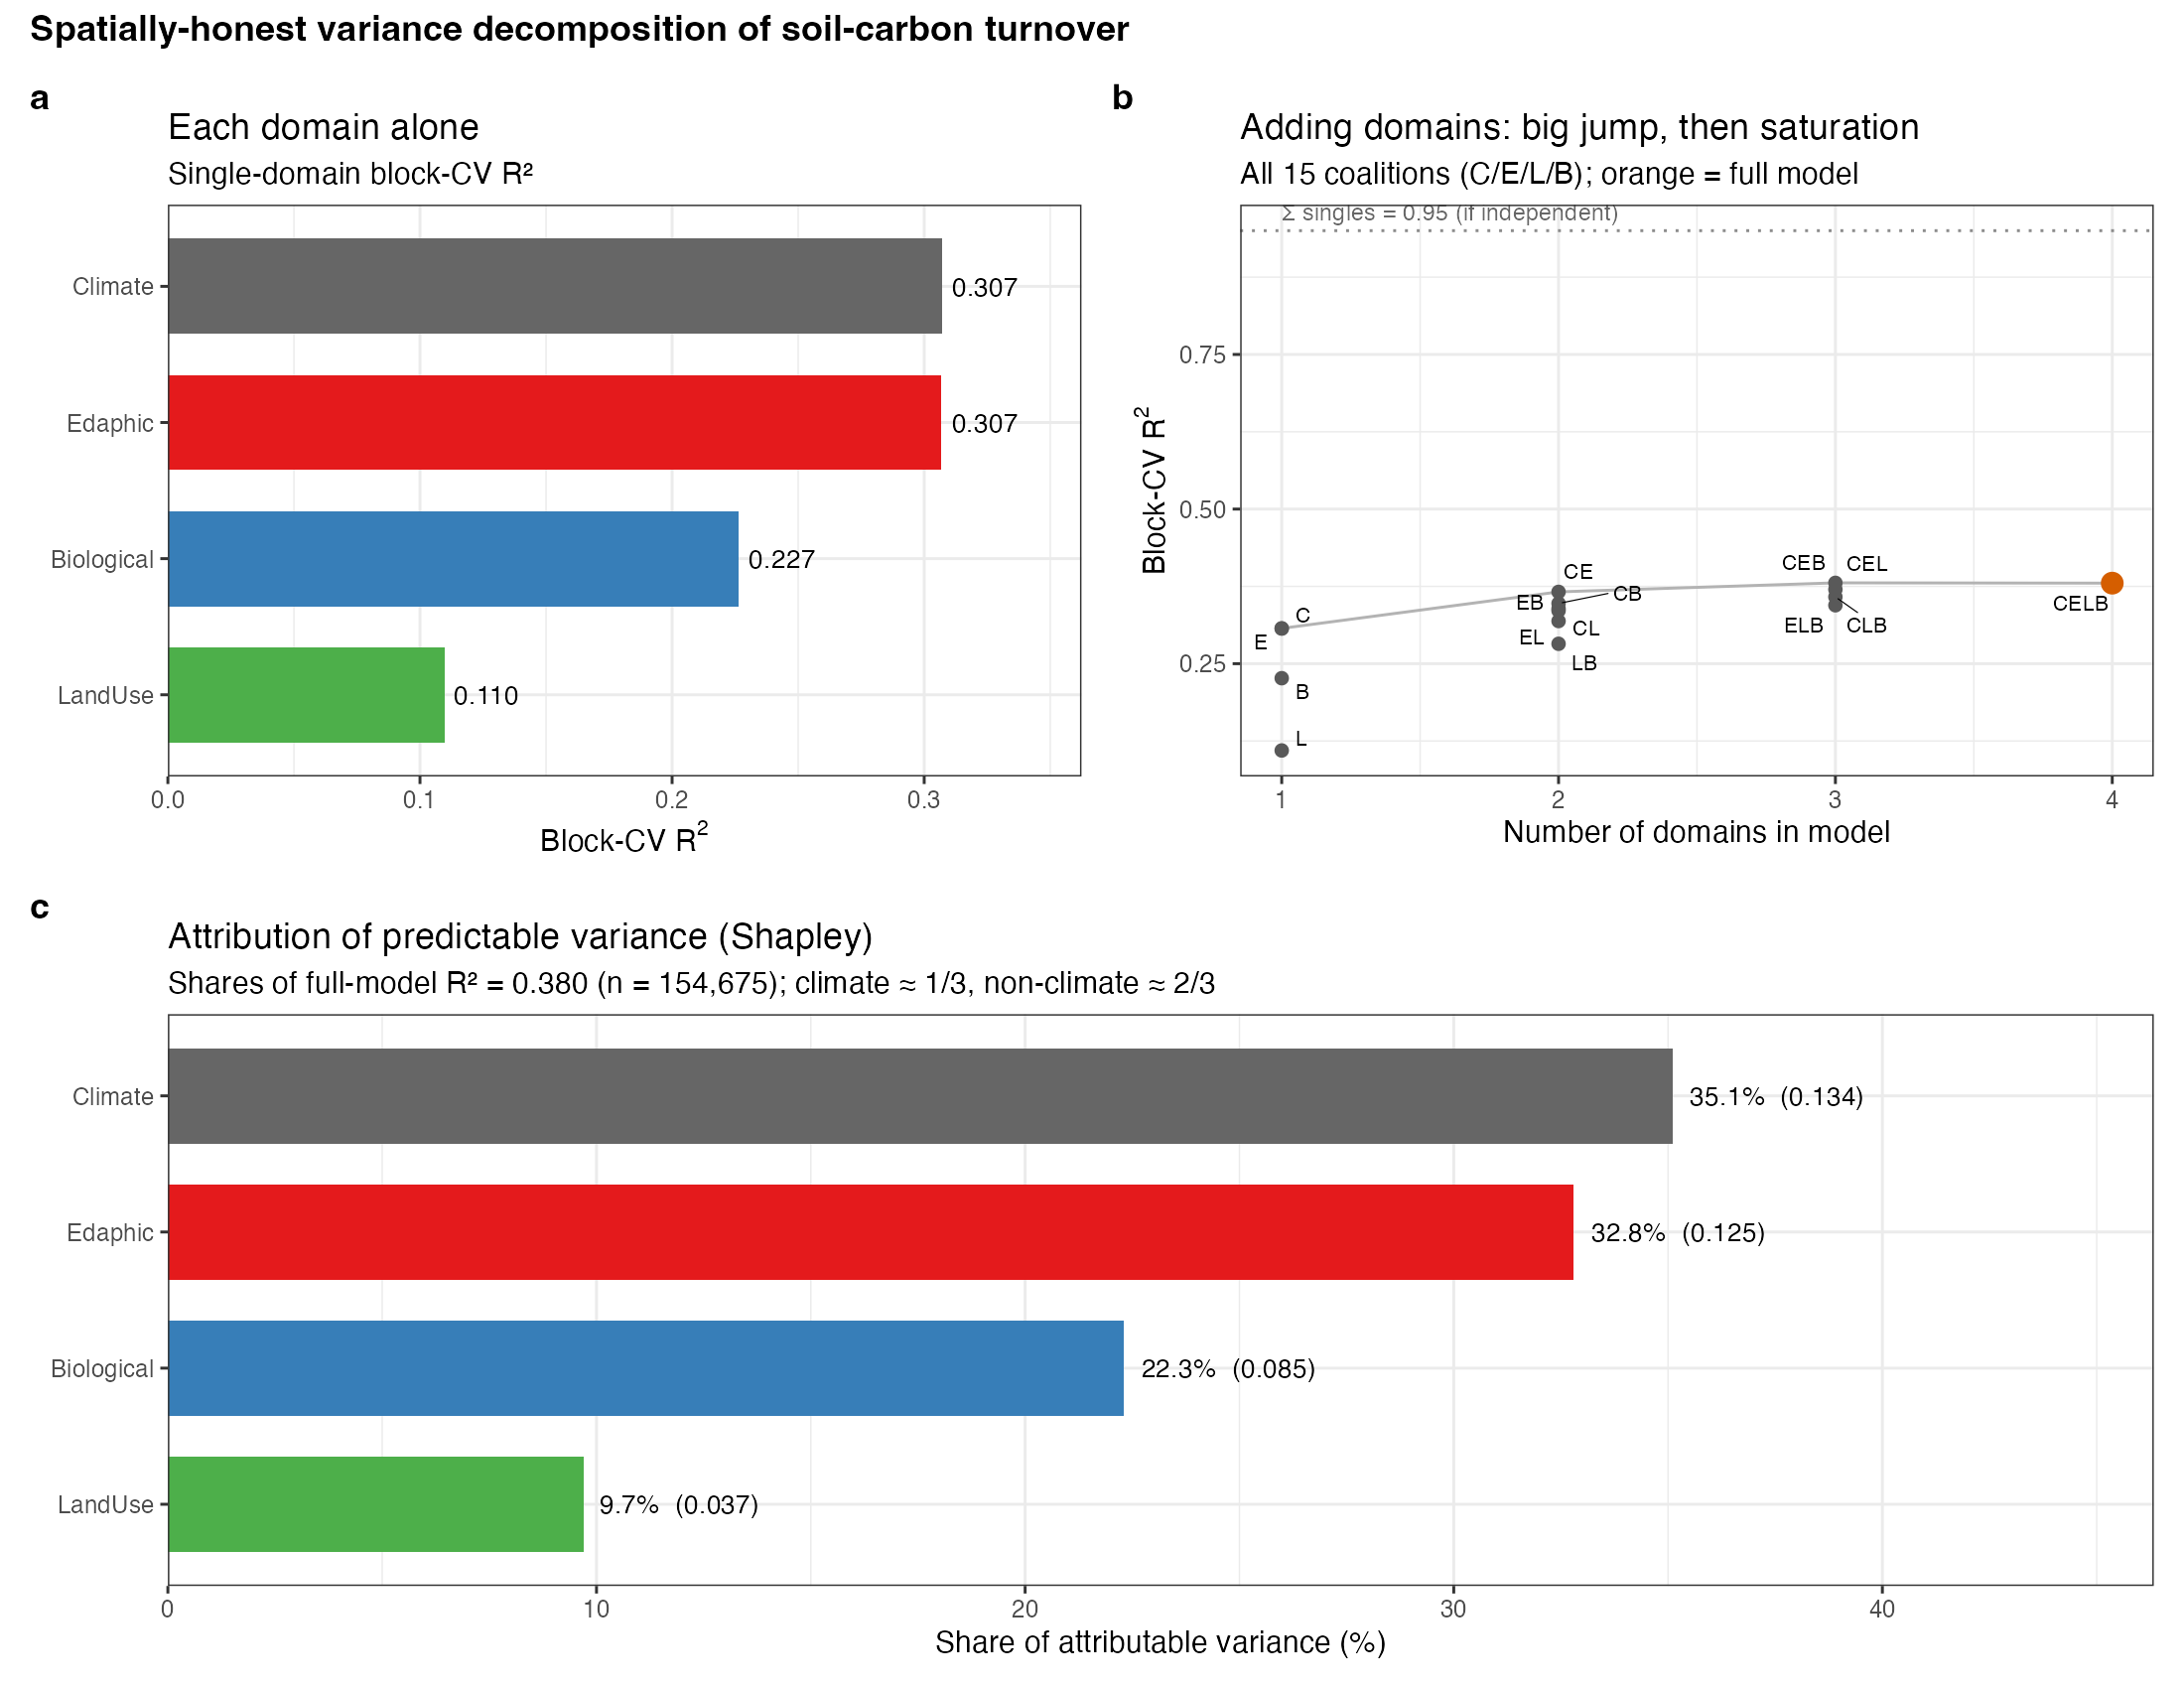
\includegraphics[width=0.92\textwidth]{../plots/step_13c_commonality/13c_decomposition.png}
\caption{\textbf{Attribution of variance among process classes.} Single-domain skill, coalition build-up, and order-independent Shapley shares (Climate~35, Edaphic~33, Biological~22, Land use~10\,\%) on the common row set ($n=150{,}863$). The full model sits well below the sum of single-domain skills: the overlap that marks correlated-but-not-redundant predictors.}
\label{fig:shapley}
\end{figure}

The single-domain skills (each group's $R^2$ on its own,
Sec.~\ref{sec:shapley}) tell the same story from another angle, and the two
analyses agree closely on the ranking. Edaphic predictors alone explain as much
variance as climate alone (both $R^2\approx0.32$), with biology next
($R^2=0.23$) and land use last ($R^2=0.11$), the same order the Shapley
decomposition gives. The single domains sum to $0.98$, far exceeding the
full-model $0.39$; the resulting overlap of $0.59$ shows that the groups are
strongly correlated but not redundant, consistent with the zonal coupling
between climate and soil (Sect.~\ref{sec:intro}). This same overlap is why the
climate-only model already reaches a relatively high $R^2=0.319$: much of that
stand-alone skill is signal climate shares with the non-climate predictors, and
the Shapley step redistributes this shared explanatory power across the classes
rather than crediting it to climate, which is why climate settles at a 35\,\%
share despite its strong single-domain skill. Land use is the clearest
illustration of the difference between the two readings: it has appreciable
skill on its own ($R^2=0.11$) yet only a modest Shapley share (9.6\,\%), almost
all of which is information it shares with the edaphic and climate predictors,
so its \emph{unique} contribution once those groups are present is near zero.
Out-of-bag
skill on a model fitted to all data was higher than the cross-validated value
($R^2_\text{OOB}=0.60$ vs.\ $R^2_\text{CV}=0.39$), the expected penalty of
holding out whole 2\textdegree{} blocks rather than random points.

% -----------------------------------------------------------------------------
\subsection{Spatial organisation of the beyond-climate residual}
\label{sec:results_moran}
% -----------------------------------------------------------------------------

The beyond-climate variance is spatially organised, not random. The residual of
the climate-only model, aggregated to 2\textdegree{} blocks, has a Moran's $I$ of
0.25 (the slope of the Moran scatter in Fig.~\ref{fig:moran}; $p\ll0.001$), with
a comparable value at 5\textdegree (residual map, Fig.~\ref{fig:residmap}):
neighbouring regions carry similar beyond-climate residuals far more often than a
random arrangement would produce. Most of the residual's point-to-point variance
is nonetheless short-range and unstructured. Its empirical semivariogram (Sect.~\ref{sec:mapscale}; Fig.~\ref{fig:noisefloor}) has a high nugget (about
56\,\% of the total sill is already present at the shortest separations, i.e.\
variance that the spatial coordinates do not resolve) and a short correlation
range ($\approx16$~km, the lag beyond which the semivariance stops rising),
% Comment by Aleksi: what drives a 16 km spatial-correlation range? seems long vs the
%   metre-scale autocorrelation of soil properties in earlier work; is it from the NPP
%   map / input estimation?
% RESOLVED: addressed in the sentences below -- the 16 km range is NOT intrinsic soil
%   autocorrelation but the effective resolution of the gridded predictor stack (MODIS
%   NPP, climate reanalysis, SoilGrids), which are smooth at hundreds of m to km, so the
%   residual can only express structure those inputs resolve.
so little point-level structure survives past a few tens of kilometres. This
range should not be read as intrinsic soil autocorrelation, which for many soil
properties operates at metres to tens of metres; it is instead inherited from the
gridded predictor fields that drive the model. Our covariates (MODIS-derived NPP,
climate reanalysis, and the SoilGrids products) are themselves smooth at scales of
hundreds of metres to kilometres, so the residual can only express structure that
those inputs resolve, and the $\approx16$~km range reflects the effective
resolution of the predictor stack rather than a property of the soils sampled. The
organised signal is therefore a meso-scale property: the agreement between the
mapped and the observed residual roughly doubles from the noisy native pixel
($R^2\approx0.11$) to $\approx0.22$ at 1--2\textdegree{} and then plateaus
(RF mapping-skill curve, Fig.~\ref{fig:mapskill}), which is the scale at which we
map it below.

\begin{figure}[H]\centering
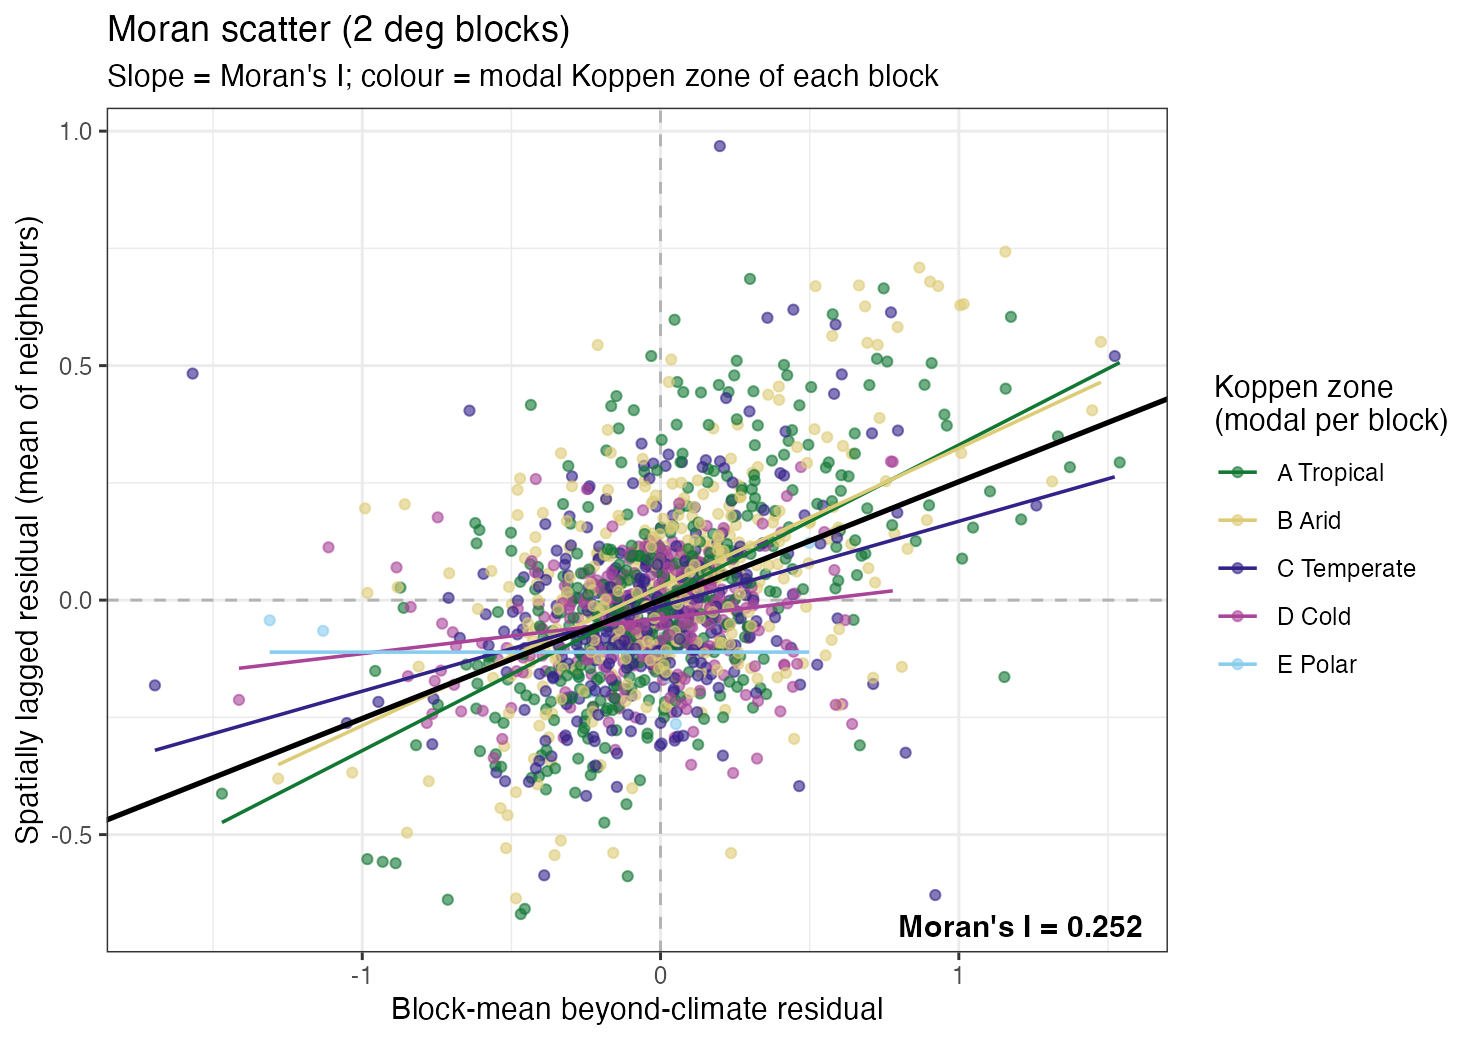
\includegraphics[width=0.6\textwidth]{../plots/step_13c_commonality/13e_moran_scatter.png}
\caption{\textbf{Spatial organisation of the beyond-climate residual.}
How to read it: each point is a 2\textdegree{} block; the horizontal axis is that block's mean beyond-climate residual (observed minus climate-only prediction), and the vertical axis is the average residual of its neighbouring blocks. A positive slope means blocks resemble their neighbours more than a random arrangement would give (spatial clustering) and the slope is Moran's $I=0.25$ ($p\ll0.001$). A flat, shapeless cloud would indicate no spatial organisation. Points are coloured by each block's modal coarse K\"oppen zone (A tropical, B arid, C temperate, D cold, E polar), and the thin coloured lines are within-zone linear fits. The beyond-climate autocorrelation is present across zones rather than confined to one, but not uniformly: the within-zone slope is steepest in tropical and arid blocks, shallower in temperate and cold ones, and essentially flat in the (few) polar blocks.}
\label{fig:moran}
\end{figure}

\subsection{Global distribution of predicted $\tau$}
\label{sec:results_map}
% -----------------------------------------------------------------------------

The full-model (M7) prediction, generated at 0.1\textdegree{} resolution,
covers ${\sim}$901\,000 land pixels and yields a global mean $\tau$ of 23.5~yr
(median 23.0~yr; Fig.~\ref{fig:global_mrt}). Predicted values span
3.9--72.8~yr across the global domain. A first-order latitudinal gradient is visible in
the predicted-$\tau$ map (Fig.~\ref{fig:global_mrt}), consistent with temperature
control on decomposition: the shortest values (below 15~yr) lie in tropical lowland
forests and intensively managed croplands, the longest (above 35~yr) in boreal forests,
montane terrain, and cold continental interiors. Regional structure also persists within
latitude bands; the decomposition below quantifies how much of this beyond-climate
variation is attributable to non-climatic context.

% -----------------------------------------------------------------------------
\subsection{Variable importance and process contribution}
\label{sec:results_importance}
% -----------------------------------------------------------------------------

Permutation importance in the full model (M7) was dominated by three climate
variables (temperature seasonality 0.367, snow cover 0.279, and soil
temperature 0.215) then AM fungal endemism (0.156), soil pH (0.151), terrain
elevation (0.147), and sand (0.141). By group, Edaphic carried the largest total
importance (1.32 over 13 variables), then Climate (1.15 over 6), Biological (0.61
over 6), and Land use (0.45 over 8). On a per-predictor basis the picture
changes: climate ranked highest per variable, but each of the six biological
layers carried about as much importance as each edaphic variable, so the
biological group contributes a large amount of importance per layer despite
being a small set.

A complementary, spatial view comes from the per-pixel magnitude by which each
non-climate group shifts the climate baseline: $|M_i - M_1|$, the absolute change
in predicted $\tau$ when group $i$ is added to the climate-only model, evaluated
at every land pixel and summarised here as global statistics (the corresponding
fields are shown, as log-ratios, in the zonality map of Fig.~\ref{fig:zonality}).
Mean absolute adjustments are 4.6~yr (Edaphic),
7.6~yr (Land use), and 4.5~yr (Biological), with maxima of 69, 93, and 79~yr. The fields
have different spatial signatures: edaphic adjustment is pervasive but moderate, largest
on strong soil-property gradients (mountains, Nordic and boreal soils, the Mediterranean,
Central Asian drylands, the Pampas--Patagonia transition); land-use adjustment is largest
per pixel but localised at land-cover boundaries (agricultural belts, deforestation
fronts, fire mosaics); biological adjustment is comparable to the edaphic one in mean
magnitude but more spatially diffuse, spread broadly across regions rather than
concentrated on sharp gradients or boundaries.

Consistent with its near-zero unique variance, land use produces the largest local shifts yet adds little that edaphic and climate do not already carry. We also note that, although the abiotic and biological panels of the zonality map (Fig.~\ref{fig:zonality}) look broadly similar, this resemblance is mostly the climate signal they share: each panel is a domain expressed relative to climate, so both inherit the same climatic backbone and co-vary ($r\approx0.4$--0.5). When biology is instead added \emph{on top of} the climate-plus-edaphic model (the nested decomposition, Fig.~\ref{fig:nestedmap}), the biological increment (what biology contributes beyond climate and edaphic context combined) is essentially uncorrelated with the abiotic field ($r\approx0$; Fig.~\ref{fig:bioscatter}). In that sense soil biology forms a distinct spatial axis rather than a restatement of the edaphic one.

\begin{figure}[H]\centering
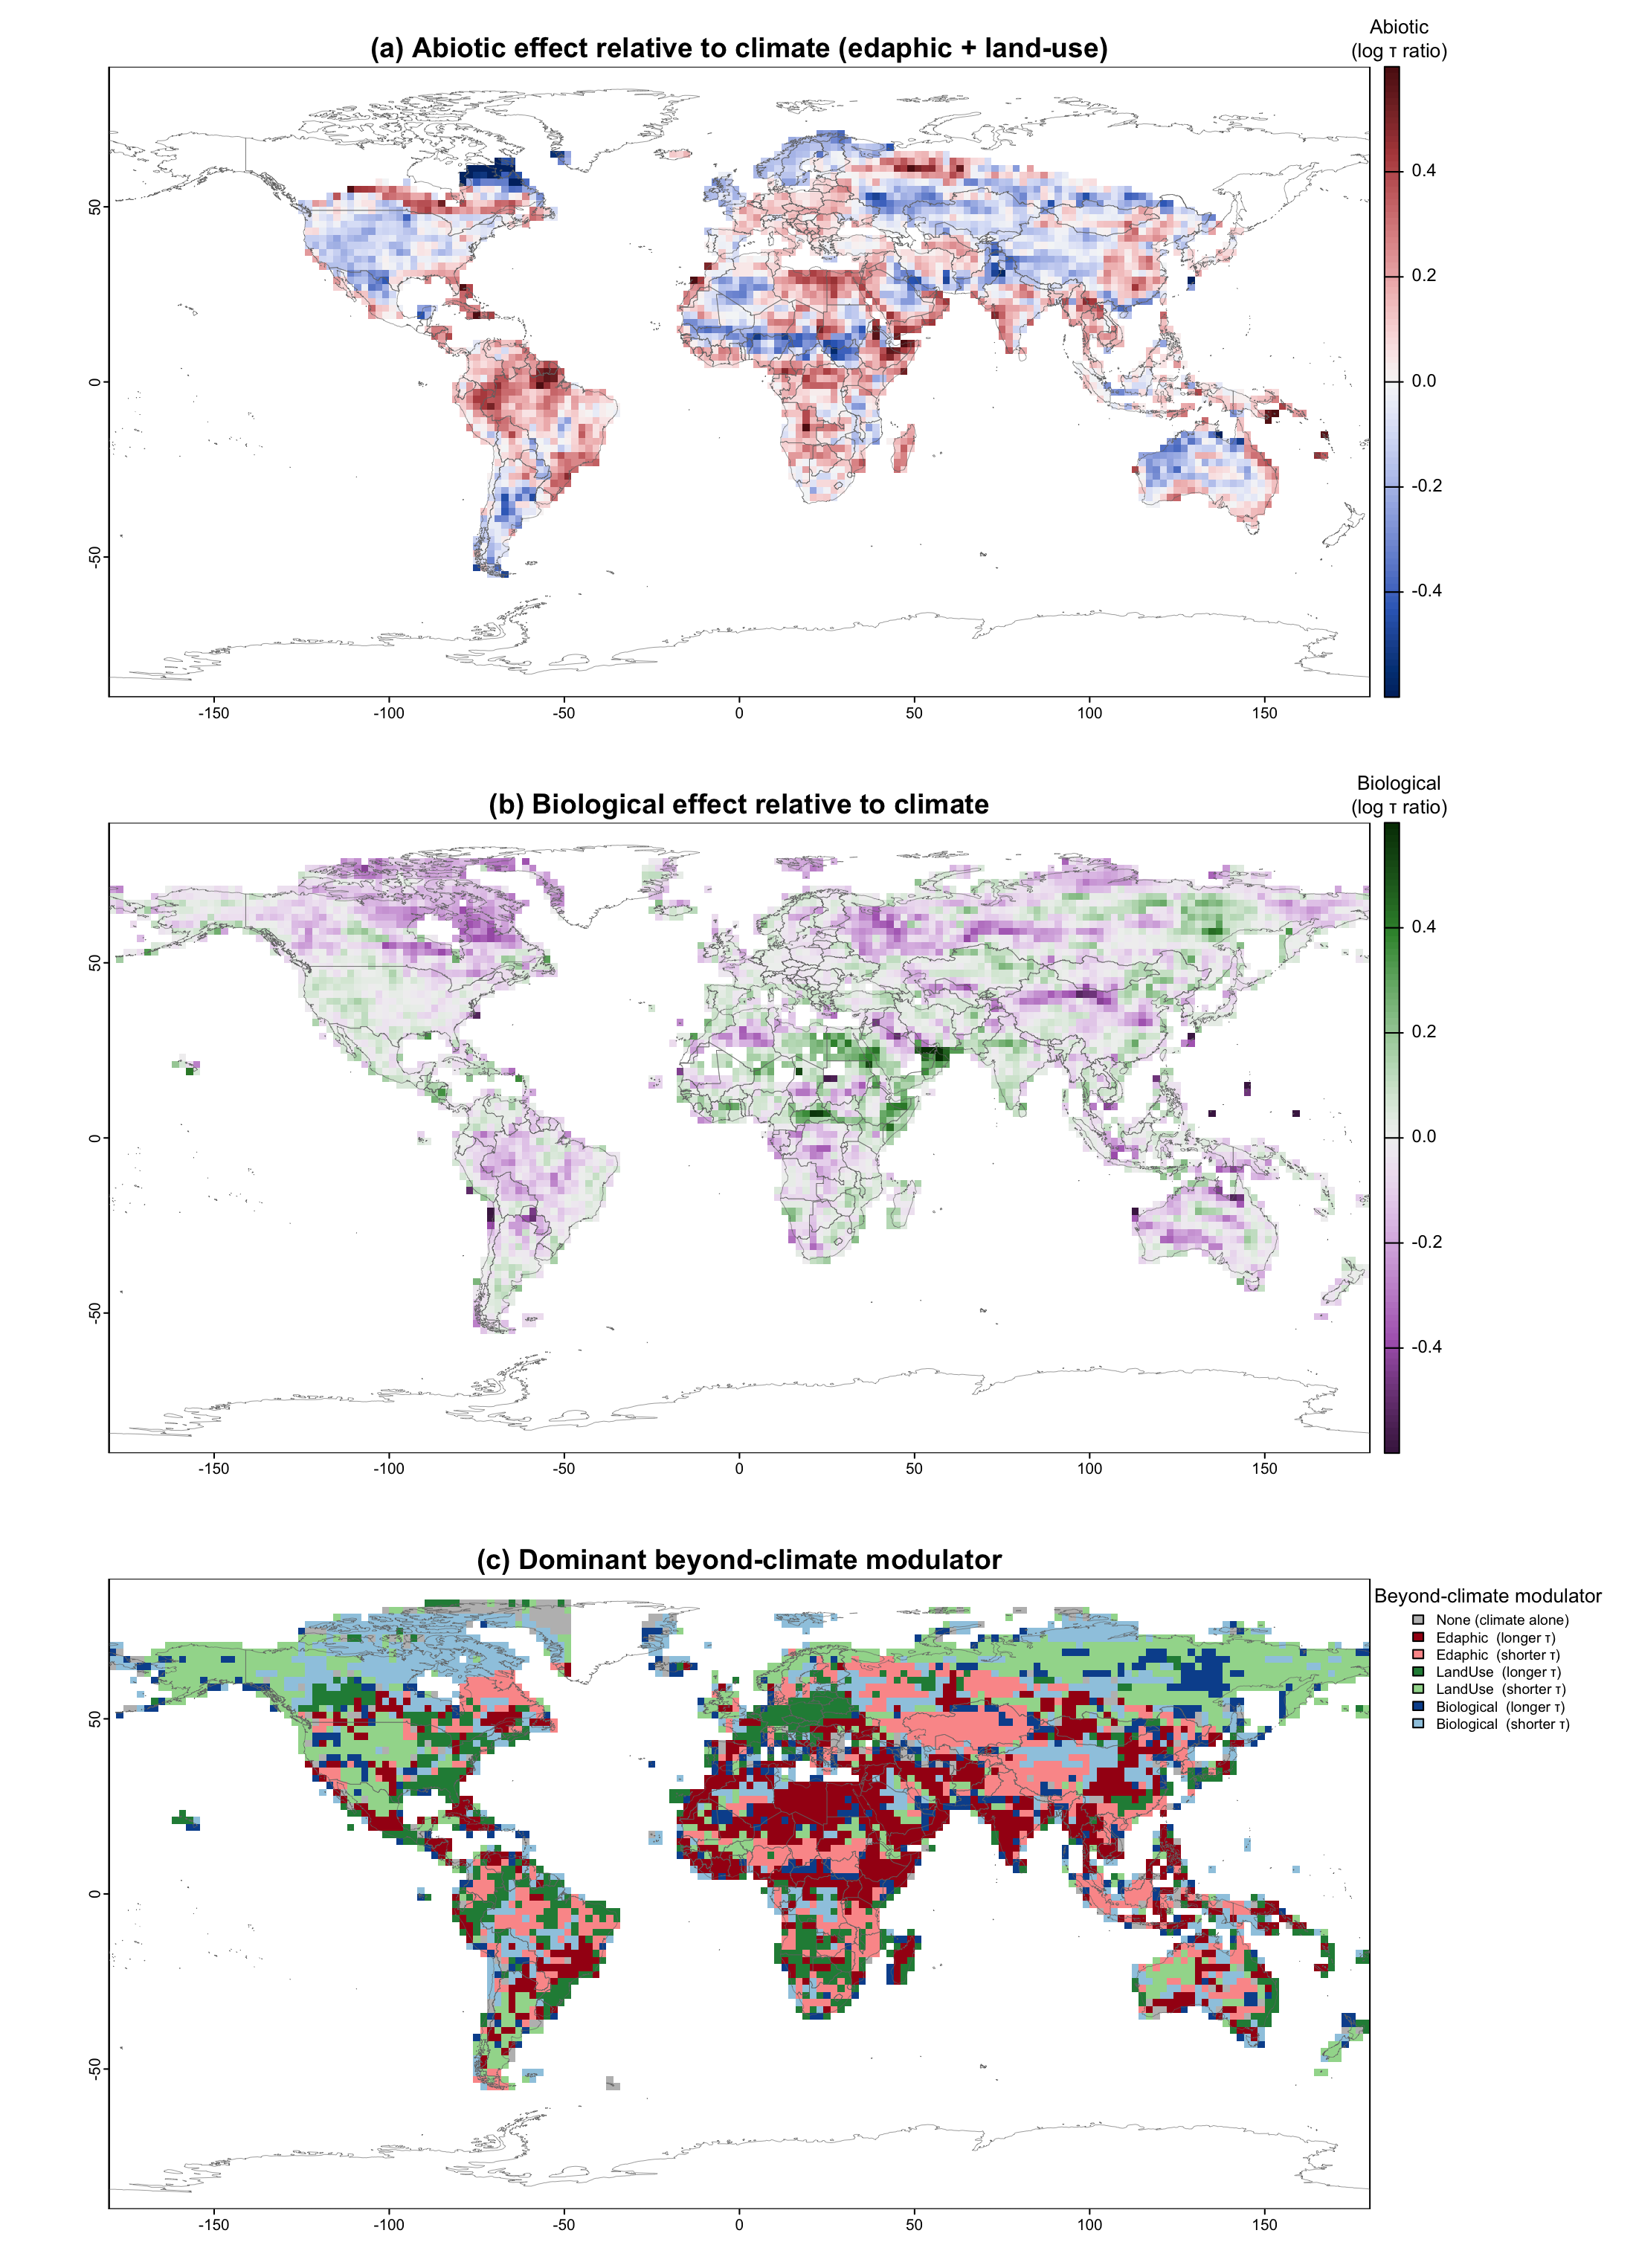
\includegraphics[width=0.9\textwidth]{../plots/step_15b_zonality/zonality_three_panel.png}
% Comment by Aleksi: caption should explain how to read the figure for non-specialists.
% RESOLVED: caption now carries an explicit "How to read it" walkthrough (below).
% Panel (c) promoted from the appendix (Lorenzo). Caption states climate is the baseline
% of all three panels, to avoid the false reading that grey = "climate is weak".
\caption{\textbf{Zonality of soil-carbon turnover.} (a)~Abiotic (edaphic + land-use) and (b)~biological modulation of $\tau$ relative to climate, at meso (2\textdegree) scale: the log-ratio of the full-model to the climate-only prediction per block (red/green~=~longer turnover, blue/purple~=~shorter). (c)~Dominant non-climate modulator per block (largest Shapley-weighted log-ratio), shaded by direction (darker~=~longer, lighter~=~shorter); grey~=~climate alone. Climate is the largest single control everywhere and the baseline of all panels: a coloured block in (c) marks where a non-climate domain most shapes the departure from climate, not where climate is unimportant.}
\label{fig:zonality}
\end{figure}

% ============================================================================
% STORYLINE DECISIONS for panel (c). Kept here: these are narrative choices, not
% plotting details.
%
% DECISION 1 -- how "dominant" is defined (2026-07-07). At each 2-deg block we have
%   three beyond-climate modulation magnitudes |log M_{clim+domain}/M_clim| (edaphic,
%   land-use, biological). We compared THREE ways to pick the dominant domain and
%   chose the one most consistent with the paper's Shapley attribution:
%     A. Raw magnitude (max |log-ratio|). REJECTED: land use "dominates" ~62% of
%        blocks, but that magnitude is mostly the imprint of the land-use carbon-
%        allocation coefficient on tau, not genuine dominance -- misleading.
%     C. SD-standardised (|log-ratio| / per-domain SD). Removes scale differences but
%        is untethered from how much each domain actually explains globally.
%     D. Shapley-weighted (|log-ratio| x domain Shapley share). CHOSEN: weights each
%        local modulation by the domain's globally attributed importance, so the
%        zonation is consistent with the Shapley decomposition the paper rests on and
%        recovers the pedologically coherent story (edaphic = drylands/temperate,
%        land use = wet + boreal forests, biology = cold high-latitude margins).
%        Class shares ~E36/L34/B26, "climate alone" ~4-5%.
%
% DECISION 2 -- avoiding a false narrative (2026-07-09). Because climate is the
%   BASELINE (subtracted) at every block, the "climate alone" class is small (~4.5%),
%   which could read as "climate is unimportant" (it is the largest single control).
%   Options: (A, CHOSEN) reframe -- retitle "beyond-climate", relabel grey
%   "Climate-dominated" -> "None (climate alone)", and state in caption + Methods that
%   climate is the baseline of all panels; (B) raise the threshold so more blocks go
%   grey -- REJECTED as cosmetic; (C) add climate as a 4th competing category --
%   REJECTED, climate is the denominator of the log-ratio units and has no comparable
%   class. The figure is intrinsically a beyond-climate decomposition.
% ============================================================================

% -----------------------------------------------------------------------------
\subsection{Marginal effects on $\tau$}
\label{sec:results_ale}
% -----------------------------------------------------------------------------

Accumulated Local Effects (ALE) analysis quantified the marginal
response of $\tau$ to each continuous predictor across its observed range
(Fig.~\ref{fig:ale_top10}). The three largest ALE effect ranges again
belonged to climate variables: temperature seasonality (9.8~yr),
snow cover (7.9~yr), and soil temperature (6.7~yr). Among non-climate
predictors, sand content gave the largest edaphic response (5.3~yr),
followed at lower magnitude by soil pH (2.2~yr) and nitrogen (1.9~yr);
tree cover (2.9~yr) was the leading land-use response and AM endemism
(2.6~yr) the leading biological one, with potential evaporation (2.4~yr)
also entering the top ten.

\begin{figure}[H]\centering
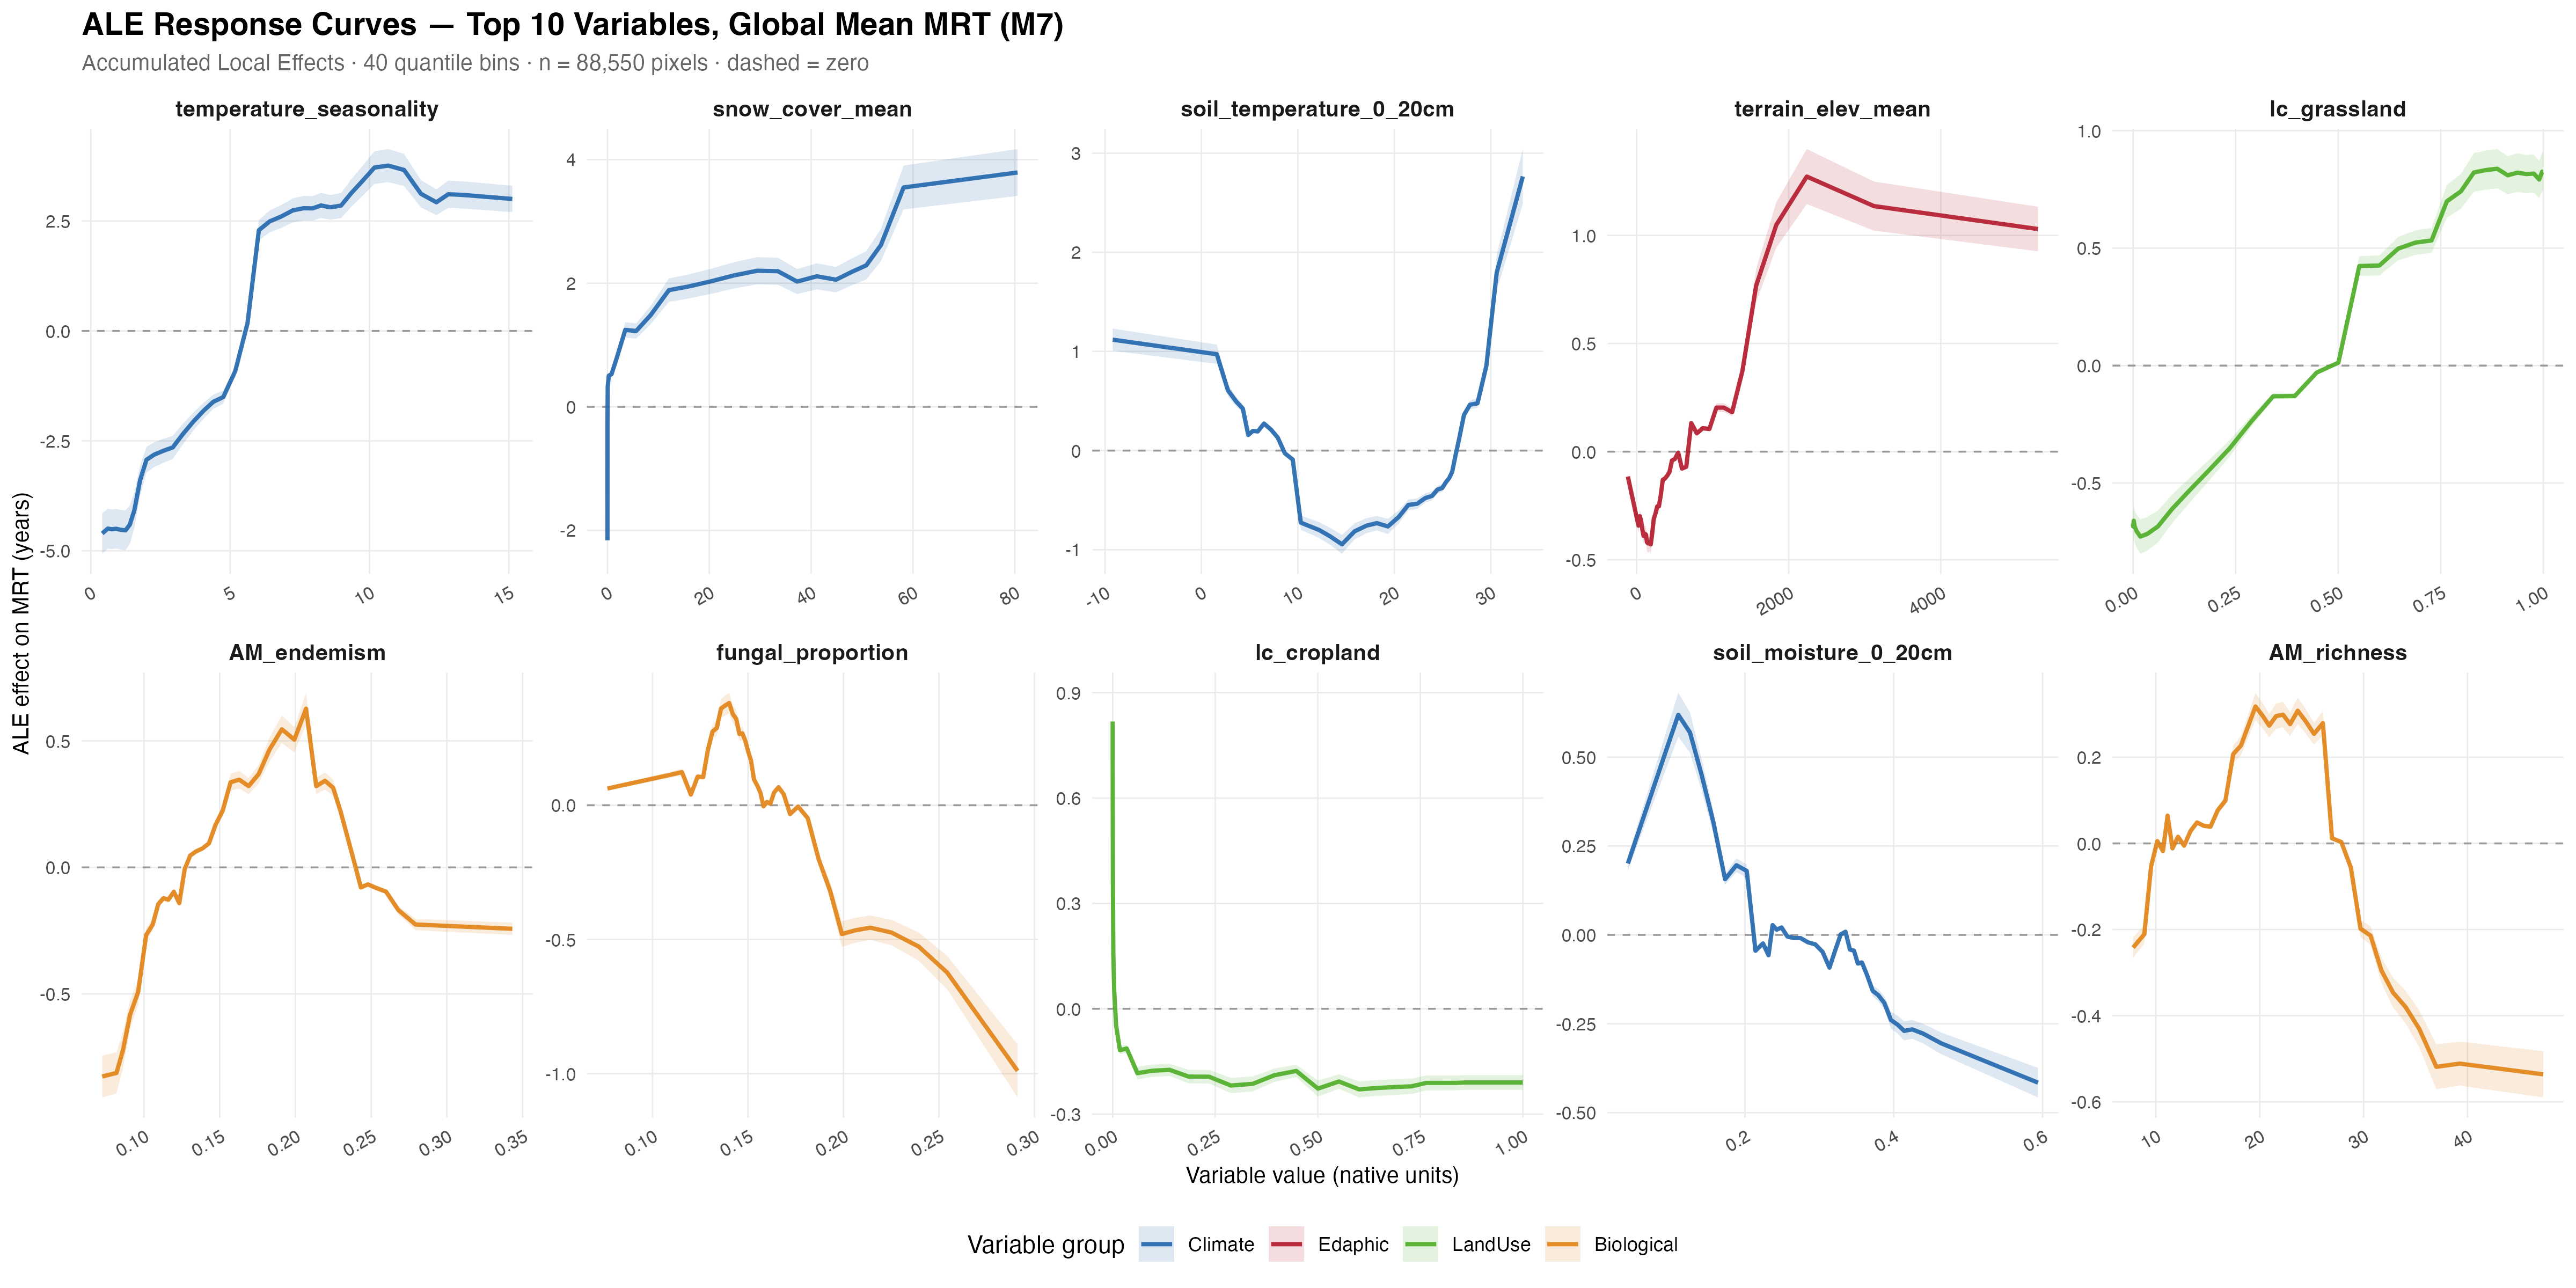
\includegraphics[width=1.0\textwidth]{../plots/step_18_sensitivity/18D_ALE_top10_MRT.png}
\caption{\textbf{ALE response curves} for the ten most responsive predictors of
$\tau$ (full model, M7). Panels are ordered by decreasing ALE range (the vertical
span of each curve, i.e.\ how much $\tau$ shifts across the predictor's observed
range), so the most influential predictors appear first; the leaders are climatic
(temperature seasonality, snow cover, and soil temperature), with sand the
strongest edaphic response. The $y$-axis is shared across panels, so the vertical span
of each curve is directly comparable: a flatter curve means a predictor moves
$\tau$ less. The $x$-axis is in each predictor's native units and therefore
differs between panels.}
\label{fig:ale_top10}
\end{figure}

The response shapes are varied (Fig.~\ref{fig:ale_top10}): temperature seasonality
saturates (rising from 1--6~K, flat above $\sim$10~K), snow cover lengthens
turnover monotonically with its steepest rise in the upper range (the effect
climbs sharply between roughly 50 and 60\,\% snow-cover fraction), and soil
temperature is U-shaped (a shape we revisit in the Discussion, where the
high-temperature upturn may partly reflect drier conditions in the hottest soils);
sand declines monotonically
(clay-rich to sand-rich shortens $\tau$ by nearly 5~yr), bulk density is threshold-like
below $\sim$1~g\,cm$^{-3}$, pH is a rising inverted-U peaking near 7.5--8, fungal
proportion drops $\tau$ above a $\sim$0.2 biomass fraction, and AM endemism is inverted-U.
The mechanistic reading of these shapes is taken up in the Discussion.

Resolved by latitude band (Fig.~\ref{fig:ale_latband}), the
temperature-seasonality response is strongest in the Boreal/Arctic zone and
near-zero in the Tropics, a zonal pattern echoed by pH (steepest in
boreal/northern-temperate soils), while the biological responses (AM endemism,
fungal proportion) are comparatively uniform across bands. We take up the
interpretation of this contrast in the Discussion.

% -----------------------------------------------------------------------------
\subsection{Comparison with ESM spatial structure}
\label{sec:results_esm}
% -----------------------------------------------------------------------------

Compared with the six-member CMIP6 ensemble, our map diverges in both magnitude and
organisation. In absolute terms the ESMs span a far wider zonal-mean range
(Fig.~\ref{fig:esm_profile}): $\sim$5--10~yr in the tropics to several hundred years
at high northern latitudes (CESM2, IPSL-CM6A-LR, MPI-ESM1-2-LR exceed 1000~yr in polar
bands; a 50--100-fold range), versus $\sim$15--50~yr for RF~M7 (3--5-fold). The
dispersion statistics (Table~\ref{tab:esm_dispersion}) confirm larger absolute spatial
variance in the ESMs, skewed towards a polar tail: the models diverge from one another
most strongly at high latitudes, where their turnover times span orders of magnitude,
and converge towards the tropics.

Rescaling each product to its own range isolates structure from magnitude
(Fig.~\ref{fig:esm_heatmap}). The ensemble mean and four of six LSMs (CESM2,
UKESM1-0-LL, IPSL-CM6A-LR, MPI-ESM1-2-LR) place most of their latitudinal domain
(tropics through boreal) in the lower part of their own range, with the high end
confined to a narrow high-northern band; only CanESM5 and MIROC-ES2L show a gradual
gradient, and MPI adds a spurious arid subtropical maximum near 20--30\textdegree{}~N.
RF~M7, by contrast, distributes structure across all latitudes.

The ESMs differ from the estimate of this study, and from one another, on
both the magnitude and the organisation of $\tau$. Indeed they span more than an
order of magnitude among themselves in absolute terms. Because absolute magnitude is not
comparable across products (their soil depths, pool definitions, and reference periods
differ), we restrict the comparison to the normalised structure. There the contrast is
in where variation sits: the models place most of it in a high-latitude extreme, whereas
in the present study it is spread across biomes (Fig.~\ref{fig:esm_biome}). In our
estimate the polar-to-tropical contrast in relative turnover is gentle ($\sim$2.5$\times$);
the ensemble's is steeper (median $\sim$9$\times$; from 0.6 for an inverted MPI gradient to
14 for CanESM5), about a factor of 3.7.

\begin{figure}[H]\centering
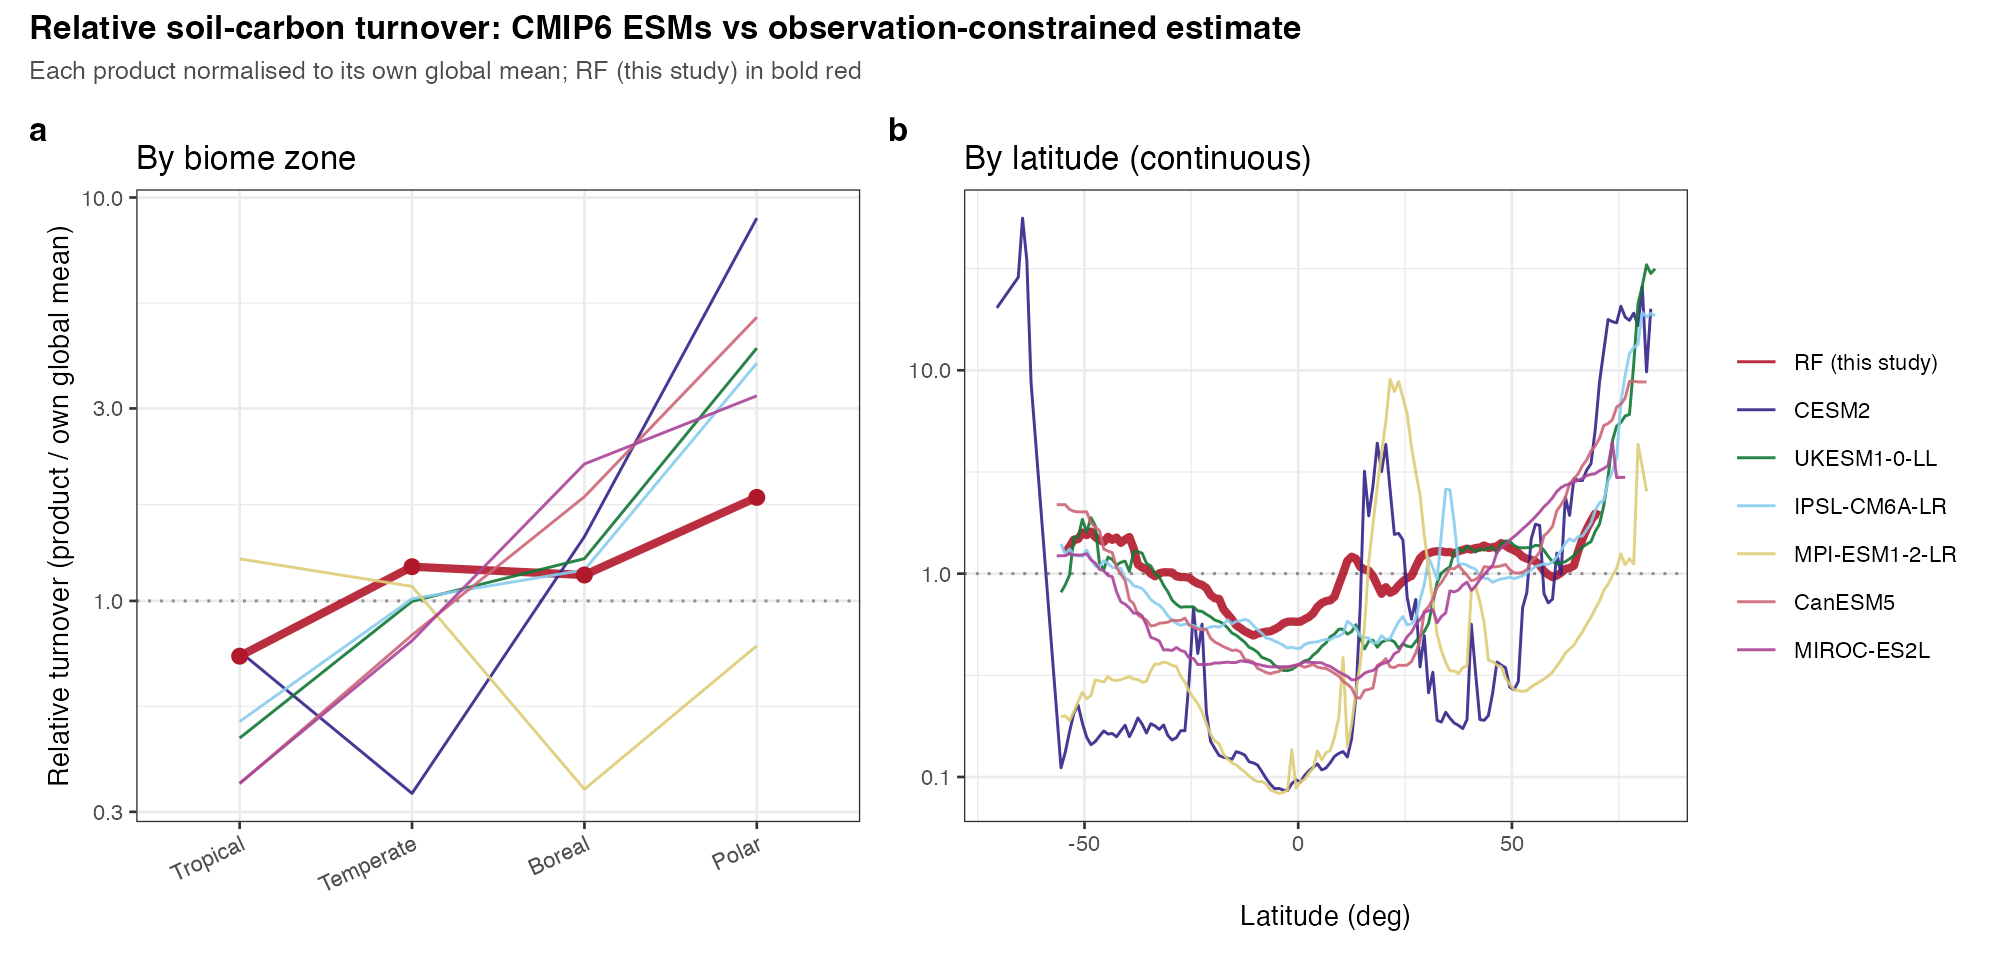
\includegraphics[width=\textwidth]{../plots/step_20/fig_esm_relative_panels.png}
\caption{\textbf{ESM structural comparison.} Relative soil-carbon turnover, each product normalised to its own global mean, shown (a)~by biome zone and (b)~as continuous latitudinal profiles (the same information, read discretely and continuously). Our estimate (RF, bold red) stays near its global mean across zones and latitudes, whereas the CMIP6 models rise steeply towards the poles (median polar/tropical contrast $\sim$9$\times$ vs $\sim$2.5$\times$ for RF; range 0.6--14$\times$, including an inverted MPI gradient).}
\label{fig:esm_biome}
\end{figure}


% =============================================================================
\section{Discussion}
% =============================================================================

\paragraph{Climate dominates, but not alone.}
The decomposition confirms climate as the leading control (temperature
seasonality, snow cover, and soil temperature top both permutation importance and
ALE), yet climate accounts for only about a third of the variance the model can
attribute (Shapley 35\,\%; single-domain $R^2=0.32$). Still, these results should not lead us to
overstating the role of non-climate context because of two reasons. 
First, ``attributable variance''
here means the predictable variance the full model captures (its spatially-honest
$R^2=0.39$ of the total variance in $\ln\tau$), partitioned among the four groups
by the Shapley decomposition (Sec.~\ref{sec:shapley}); it is not the total
variance in $\tau$, most of which stays unpredictable at this resolution. The
``two thirds'' attributed to non-climate classes are therefore shares of that
39\,\%, not of all variation. Second, in absolute terms the non-climate groups add
only about 7 percentage points of explained variance over climate alone ($R^2$
rising from 0.32 to 0.39), because climate and the other groups carry heavily
overlapping signals (Sec.~\ref{sec:results_models}), a reflection of the zonal
coupling between climate and soil noted earlier (Sec.~\ref{sec:intro}). The beyond-climate
contribution is thus real and, as we show next, spatially organised, but modest in
absolute predictive terms rather than a wholesale rewriting of the climate
account. One caveat on reading the climate response shapes: the soil-temperature
ALE is U-shaped, turning back upward at the highest temperatures, but the hottest
soils in our data are also the driest (Pearson $r\approx-0.24$ between soil
temperature and moisture; mean soil moisture falls from ${\sim}0.31$ to
${\sim}0.26$ in the warmest temperature decile). The upturn may therefore carry a
moisture signal (hot, dry soils decomposing slowly) that the marginal curve cannot
fully separate from a direct thermal effect; a two-way temperature--moisture ALE
would be needed to resolve it.

This residual is not noise: it is geographically organised (Fig.~\ref{fig:zonality}).

\paragraph{Edaphic context is the largest non-climate signal.}
Edaphic context is the largest non-climate term: its Shapley share (33\,\%) is very
close to climate's (35\,\%), and on its own it predicts $\tau$ as well as climate
does (single-domain $R^2=0.32$ for both). It also carries the largest non-climate
aggregate importance. That edaphic properties should rival climate is, under the
pedological reading, expected rather than surprising. Climate is itself one of the
primary soil-forming factors (Sec.~\ref{sec:intro}), so soil properties partly
encode the same zonal climate signal; the large climate--edaphic overlap in the
decomposition (Sec.~\ref{sec:results_models}) is a direct expression of that
coupling, not a redundancy to be explained away. Read this way, the edaphic signal
does not so much compete with climate as register the soil's integrated, zonally
organised response to it, together with those soil-forming influences (parent
material, relief, age) that climate scalars do not capture. Sand, pH, bulk density, and CEC all enter the top-ten ALE responses with
interpretable mechanisms: coarse texture limits organo-mineral stabilisation (faster
turnover) \PH{[cite: Six 2002; Hassink 1997]}; low bulk density tracks porous,
aggregated soils that protect carbon; and rising CEC stabilises organic matter on
mineral surfaces \PH{[cite: Rasmussen 2018; Kleber 2007]}.

\paragraph{pH as a microbial--edaphic bridge.}
pH is nominally edaphic but also controls microbial community composition, notably
the fungi-to-bacteria ratio \PH{[cite: Rousk 2010; Malik 2018; Fierer 2006]}. Its
ALE peaks near pH~7.5--8 and is strongest in northern temperate and boreal soils,
where acidic, fungi-dominated forests coincide with the short $\tau$ we predict
there. This supports reading pH, fungal proportion, and $\tau$ as one coupled axis
(lower pH, higher fungal dominance, faster bulk turnover), reinforced by the
inverse fungal-proportion/$\tau$ relationship (Fig.~\ref{fig:ale_top10}). An
alternative reading is geochemical rather than microbial: at high pH, calcium and
carbonates can lengthen turnover by stabilising organic matter directly, through
cation bridging between organic molecules and mineral surfaces and through
carbonate-related aggregation \PH{[cite: Rowley 2018 (Ca--OM); Rasmussen 2018;
Roth\'e 2019]}. We regard the microbial route as the more parsimonious of the two,
given the independent fungal signal, but the two mechanisms are not mutually
exclusive and may act together where both high pH and abundant carbonate occur.

\paragraph{Biological context through mycorrhizal structure.}
Biological variables are the second-largest non-climate term (Shapley 22\,\%) despite
the modest six-layer set. That mycorrhizal community structure should bear on turnover
is plausible on independent grounds: mycorrhizal type and biomass shape both the
quantity and the chemistry of carbon entering the soil, and fungal necromass is now
recognised as a major precursor of stable, mineral-associated organic matter,
especially in high-latitude forests \PH{[cite: Averill 2014; Clemmensen 2013;
Soudzilovskaia 2019; Frey 2019]}; the biogeography of mycorrhizal richness and
host association is itself strongly zonal \PH{[cite: Tedersoo 2014; Steidinger 2019;
Van Nuland 2025]}. Within our results the pattern is at least suggestive: AM
endemism leads, with fungal proportion and the other mycorrhizal richness/endemism
metrics close behind, and the root-colonisation layers add negligible unique skill
(Sect.~\ref{sec:robust}). One possible reading is that the biogeographic composition
and diversity of mycorrhizal communities, rather than the quantity of colonisation,
might relate to bulk turnover. The latitude-band ALE adds a small further hint: the
biological responses (AM endemism, fungal proportion) are comparatively uniform
across bands (Fig.~\ref{fig:ale_latband}), which \emph{might} indicate a mycorrhizal
influence largely independent of macroclimate, though it \emph{might} equally reflect
covariation with other biological or edaphic gradients that we cannot separate here.
We therefore flag soil biology as a faint but interesting possibility to test
directly, not an established result: the apparent signal may still be partly a
co-variation with edaphic and climatic gradients.

\paragraph{Land use: large local shifts, redundant information.}
Land use adds essentially no unique variance once edaphic and biological
context are present (Shapley 9.6\,\%, unique $\approx0$), yet produces the largest
per-pixel adjustments (mean~7.6~yr) at cropland mosaics, deforestation fronts, and
burn scars (shifts largely predictable from the soil and microbial signatures that
accompany land-use change). Whether land use causes those changes, shares drivers with
them, or merely co-varies cannot be resolved from contemporary snapshot covariates;
for predicting $\tau$, it adds little beyond the other groups.

\paragraph{Process contribution is geographically organised.}
Non-climate adjustments are organised, not scattered (Fig.~\ref{fig:zonality}):
edaphic modulation clusters in mountainous and arid-gradient regions, land use in
agricultural and disturbance mosaics, biology in the boreal and southern temperate
belts. This is the spatial signature the zonality framework anticipates: different
process classes having different importance in different biomes.

\paragraph{SOC zonality as a working framework.}
Across these results, the spatial structure of $\tau$ behaves as an emergent property of
local ecological context rather than a fixed kinetic constant scaled only by climate. Treating
the zonality of SOC turnover as a working framework, analogous to the pedogenic
zonality that organises soil classification, could represent an interpretative tool that helps draw the mechanistic findings of the past two decades into a synthesis useful for predictions. For modelling, the consequence is concrete: turnover becomes a set of region-specific sensitivities rather than a single climate-scaled law, so a meaningful share of the spatial variance in kinetics will remain unexplained by any global parameterisation. Because each process class is most expressed in a different region, such a framework would need to be spatially explicit, with region-specific combinations of climatic, edaphic, biological, and land-use modulation. The marginal-effect shapes we recover (thresholds, saturation, monotonic and
inverted-U responses) are best read not as ready-made functional forms but as hints
at what those forms might look like, and (perhaps more usefully) as a way of
sharpening the research questions and directions needed to establish them. They also
vary by biome rather than following a single global curve, which suggests that making
turnover formulations biome-aware, rather than globally uniform, could capture more
of the spatial variance: current models already perform reasonably, and this is a
route to improving them without discarding what they get right.

\paragraph{Comparison with Earth System Models.}
The contrast with the CMIP6 ensemble is one of spatial structure. (Absolute
magnitude is not meaningfully comparable across these products, given their
differing soil depths, pool definitions, and reference periods, so we do not read
anything into it.) In structure, the models place most of their spatial $\tau$
variation in a high-latitude extreme over a comparatively uniform lower-latitude
background, whereas in the present study the structure is spread across climate
zones, and the models disagree among themselves by an order of magnitude. We read
this as an inconsistency worth investigating rather than evidence that either
picture is correct. Both are ultimately grounded in data, but the ESMs reach the
$\tau$ field through fixed, globally calibrated process forms that leave little
freedom to express local variance, whereas ours lets the observed spatial
covariation of $\tau$ with its drivers do the work; this difference may itself
account for part of the divergence. One caveat tempers the comparison: our $\tau$
field is coverage-limited (blank where the global soil and biological predictors are
missing, including parts of the high latitudes), whereas the ESM fields are spatially
complete, so the two are not evaluated on identical cells; part of the apparent
difference in poleward steepness may reflect this domain mismatch rather than model
behaviour alone. It does, however, point to mid-latitude and subtropical
structure (which our analysis associates with edaphic, biological, and land-use
context) as one place where soil-carbon representations might be examined, with the
candidate functional shapes suggested here as a possible starting point.

Our finding also speaks to a prominent use of the spatial $\tau$ field.
\citet{Varney2020} constrain the warming sensitivity of soil-carbon turnover by
treating the present-day spatial relationship between $\tau$ and temperature as a
proxy for its temporal response, an emergent constraint that implies an effective
$Q_{10}\approx2.5$ and halves the CMIP uncertainty in soil-carbon loss under
2\textdegree{}C of warming. That approach presumes the spatial $\tau$--temperature
gradient is largely thermal. Our decomposition qualifies this reading: temperature
alone explains little of the point-level variation in $\tau$
(Fig.~\ref{fig:tempscatter}, $R^2=0.06$), and the beyond-climate residual is
spatially organised rather than random (Moran's $I=0.25$), carrying edaphic and
biological structure that a $\tau$--temperature curve would absorb into an apparent
thermal sensitivity. Space-for-time constraints on $\tau$ might therefore be
sharpened by first accounting for this non-thermal zonal structure. We note also
that \citeauthor{Varney2020} define turnover through respiration
($\tau=C_s/R_h$) rather than through carbon input as we do, so the two estimates are
related but not identical.

\paragraph{Limitations.}
The steady-state assumption is a simplification; we rely on non-equilibrium errors
partially cancelling across $\sim$180\,000 profiles, and the single-pool diagnostic
conflates pools \citep{Sierra2018}. BNPP allocation fractions are literature-based
constants. Sampling is spatially uneven (dense in North America/Europe, sparse in
tropical Africa and high-latitude Asia), so data-poor predictions warrant caution.
Predictor correlations among climate, edaphic, and land-use variables are inherent to
the observational design and cannot be fully disentangled without experimental or
temporal replication. Finally, depth and pool-definition differences complicate the
CMIP6 comparison, which is why we compare relative structure rather than absolute
magnitude. A large fraction of the point-to-point variance in $\tau$ also stays
unpredictable at this resolution (Sect.~\ref{sec:mapscale}; Fig.~\ref{fig:noisefloor}):
the beyond-climate signal we recover is a meso-scale, spatially organised component,
not a pixel-level reconstruction. Part of that residual is measurement and
steady-state noise, but part likely reflects fine-scale controls our global
predictors cannot resolve, chiefly the quantity and quality of carbon inputs.
Our input term is a belowground-NPP proxy that omits aboveground litter, litter
chemistry, and management removals (harvest, residue export), and these are plausibly
first-order at the local scale (though they do not affect the attributed spatial
structure: re-deriving $\tau$ under total-NPP and generous-harvest conventions leaves
the beyond-climate gap and its organisation essentially unchanged, Sec.~\ref{sec:robust});
predictors closer to the actual input flux, together
with denser and repeated sampling, would be the most direct route to reducing the
unexplained variance. These motivate time-resolved transit times, manipulative
experiments, and targeted sampling in undersampled regions.

\paragraph{Implications: a biome-aware, tractable parameterisation.}
Existing models already carry part of this variance through fixed modifiers
(texture or clay scaling of turnover, for instance). What our decomposition points
to is a further, spatially organised share arising from more complex ecological
interactions among edaphic, biological, and land-use context, which a small set of
globally fixed modifiers is unlikely to reproduce. The question is then how to
express it without over-specifying mechanism. The structure we describe need not be
operationalised by adding mechanistic complexity. A lighter route is to stratify the calibration of existing models by
biome: keeping their first-order kinetics and architecture intact, but letting the
turnover rate differ among zonal classes that combine climatic, edaphic, and
biological context. Working through calibration rather than structure, this could
recover much of the organised beyond-climate variance without imposing new
mechanistic assumptions that may not hold in a system whose processes are only
partly known. It also follows a long-standing pedological intuition
(Sect.~\ref{sec:intro}): soils are complex systems, and complex systems are seldom
well served by purely reductionist description. In the terms of the ecosystem-property
view \citep{Schmidt2011}, the beyond-climate structure is an emergent outcome of
interacting controls, and a calibration that lets turnover vary by zonal class
captures that emergence directly; adding mechanistic detail process by process risks
rebuilding the system from parts and missing what only appears at the whole-system
level. Our proposal is one concrete way to finally operationalise that emergence.
The biome-dependent response shapes
(Sect.~\ref{sec:results_ale}) indicate which classes such a scheme would need to
distinguish.

% =============================================================================
\section{Conclusions}
% =============================================================================

\PH{[PLACEHOLDER --- conclusions to be written]}
\begin{itemize}
\item \PH{Climate explains about a third of the attributable variance; non-climate context (edaphic-led, with soil biology a distinct second axis) carries two thirds.}
\item \PH{The beyond-climate signal is modest ($\sim$7~pp) but spatially organised (Moran's $I=0.25$) and ecological, not a provenance artefact.}
\item \PH{Drivers act through interpretable, biome-dependent response shapes; the zonality of turnover as a working framework with concrete parameterisation targets.}
\item \PH{ESMs show a steeper latitudinal contrast ($\sim$3.7$\times$) and disagree by an order of magnitude --- an inconsistency to investigate, not a verdict on either.}
\end{itemize}


% =============================================================================
\section*{Data availability}
% =============================================================================

Soil profile data are from the OpenLandMap Open Compendium of Soil
Datasets \citep{OpenLandMapSoilDB2025}, \url{https://zenodo.org/records/15593990}.
ERA5-Land data are available from the Copernicus Climate Data Store
(\url{https://cds.climate.copernicus.eu}).
SoilGrids data are available from ISRIC (\url{https://soilgrids.org}).
ESA WorldCover is available at \url{https://worldcover2021.esa.int}.
Hansen forest change data are available at
\url{https://earthenginepartners.appspot.com/science-2013-global-forest}.
MODIS products are available from the LP~DAAC.
Microbial datasets are available from their respective repositories as
cited in the text.

\section*{Code availability}

The complete R analysis pipeline (20~scripts) is archived at
\PH{[DOI/repository]}.

\section*{Acknowledgements}
This work was carried out as part of the NextGenCarbon project (Next Generation
Modelling of Terrestrial Carbon Cycle by assimilation of in situ campaigns and
Earth Observations), funded by the European Union under Horizon Europe grant
agreement No.~101184989. \PH{[further acknowledgements TBD]}

\section*{Author contributions}
\PH{[author contributions --- CRediT TBD]}

\section*{Competing interests}

The authors declare no competing interests.

% =============================================================================
\bibliographystyle{apalike}
\bibliography{references}
% =============================================================================



\newpage
\section*{Tables}

\begin{table}[h!]
  \centering
  \small
  \caption{%
    \textbf{Predictor variables in the full model (M7), organised by
    mechanistic group.}
    All variables were resampled to 0.1\textdegree{} for global prediction.
    Biological rows marked $\dagger$ are used only in the nine-layer
    sensitivity (Sec.~\ref{sec:robust}), not in M7.
  }
  \label{tab:predictors}
  \begin{tabularx}{\textwidth}{lllX}
    \toprule
    Group & Variable & Units & Source \\
    \midrule
    \multirow{6}{*}{\rotatebox{90}{\textbf{Climate}}}
      & Soil temperature (0--20\,cm)    & \textdegree{}C    & ERA5-Land (depth-weighted stl1/stl2) \\
      & Temperature seasonality         & K     & ERA5-Land (monthly SD of t2m) \\
      & Soil moisture (0--20\,cm)       & m$^3$\,m$^{-3}$ & ERA5-Land (depth-weighted swvl1/swvl2) \\
      & Snow cover fraction             & 0--1             & ERA5-Land \\
      & Potential evaporation            & m                & ERA5-Land \\
      & K\"oppen-Geiger zone            & 1--30            & \citet{Beck2023}, 1991--2020 \\
    \midrule
    \multirow{13}{*}{\rotatebox{90}{\textbf{Edaphic}}}
      & Clay content                    & \%               & SoilGrids 250\,m v2.0, 0--20\,cm \\
      & Sand content                    & \%               & SoilGrids 250\,m v2.0, 0--20\,cm \\
      & Bulk density                    & kg\,dm$^{-3}$    & SoilGrids 250\,m v2.0, 0--20\,cm \\
      & Coarse fragment volume          & \%               & SoilGrids 250\,m v2.0, 0--20\,cm \\
      & pH (H$_2$O)                     & ---              & SoilGrids 250\,m v2.0, 0--20\,cm \\
      & Cation exchange capacity        & cmol\,kg$^{-1}$  & SoilGrids 250\,m v2.0, 0--20\,cm \\
      & Total nitrogen                  & g\,kg$^{-1}$     & SoilGrids 250\,m v2.0, 0--20\,cm \\
      & WRB functional group            & 1--8             & SoilGrids WRB, reclassified \\
      & Elevation                       & m                & Copernicus GLO-30 DEM \\
      & Slope                           & \textdegree{}     & Copernicus GLO-30 DEM \\
      & Northness                       & $-1$ to $+1$     & Copernicus GLO-30 DEM \\
      & Eastness                        & $-1$ to $+1$     & Copernicus GLO-30 DEM \\
      & Terrain ruggedness              & m                & Copernicus GLO-30 DEM (focal SD) \\
    \midrule
    \multirow{8}{*}{\rotatebox{90}{\textbf{Land Use}}}
      & Tree cover fraction             & 0--1             & ESA WorldCover 2021 \\
      & Grassland fraction              & 0--1             & ESA WorldCover 2021 \\
      & Shrubland fraction              & 0--1             & ESA WorldCover 2021 \\
      & Cropland fraction               & 0--1             & ESA WorldCover 2021 \\
      & Bare/sparse fraction            & 0--1             & ESA WorldCover 2021 \\
      & Wetland fraction                & 0--1             & ESA WorldCover 2021 \\
      & Forest loss (binary)            & 0/1              & Hansen GFC v1.10 \\
      & Fire count (pre-sampling)       & count            & MODIS MCD64A1, 2001--2020 \\
    \midrule
    \multirow{9}{*}{\rotatebox{90}{\textbf{Biological}}}
      & Fungal proportion               & 0--1             & \citet{Yu2022} \\
      & AM root colonisation$^\dagger$  & \%               & \citet{Barcelo2023} \\
      & EcM root colonisation$^\dagger$ & \%               & \citet{Barcelo2023} \\
      & EcM:AM root ratio$^\dagger$     & ---              & Derived from above \\
      & AM fungal richness              & index            & \citet{VanNuland2025} (SPUN) \\
      & EcM fungal richness             & index            & \citet{VanNuland2025} (SPUN) \\
      & AM endemism (RWR)               & index            & \citet{VanNuland2025} (SPUN) \\
      & EcM endemism (RWR)              & index            & \citet{VanNuland2025} (SPUN) \\
      & EcM:AM richness ratio           & ---              & Derived from above \\
    \bottomrule
  \end{tabularx}
\end{table}


% =============================================================================
% SUPPLEMENTARY MATERIAL
% =============================================================================

\newpage
\setcounter{figure}{0}
\renewcommand{\thefigure}{A\arabic{figure}}
\setcounter{table}{0}
\renewcommand{\thetable}{A\arabic{table}}

\section*{Appendix}

\subsection*{Appendix figures}

\begin{figure}[H]\centering
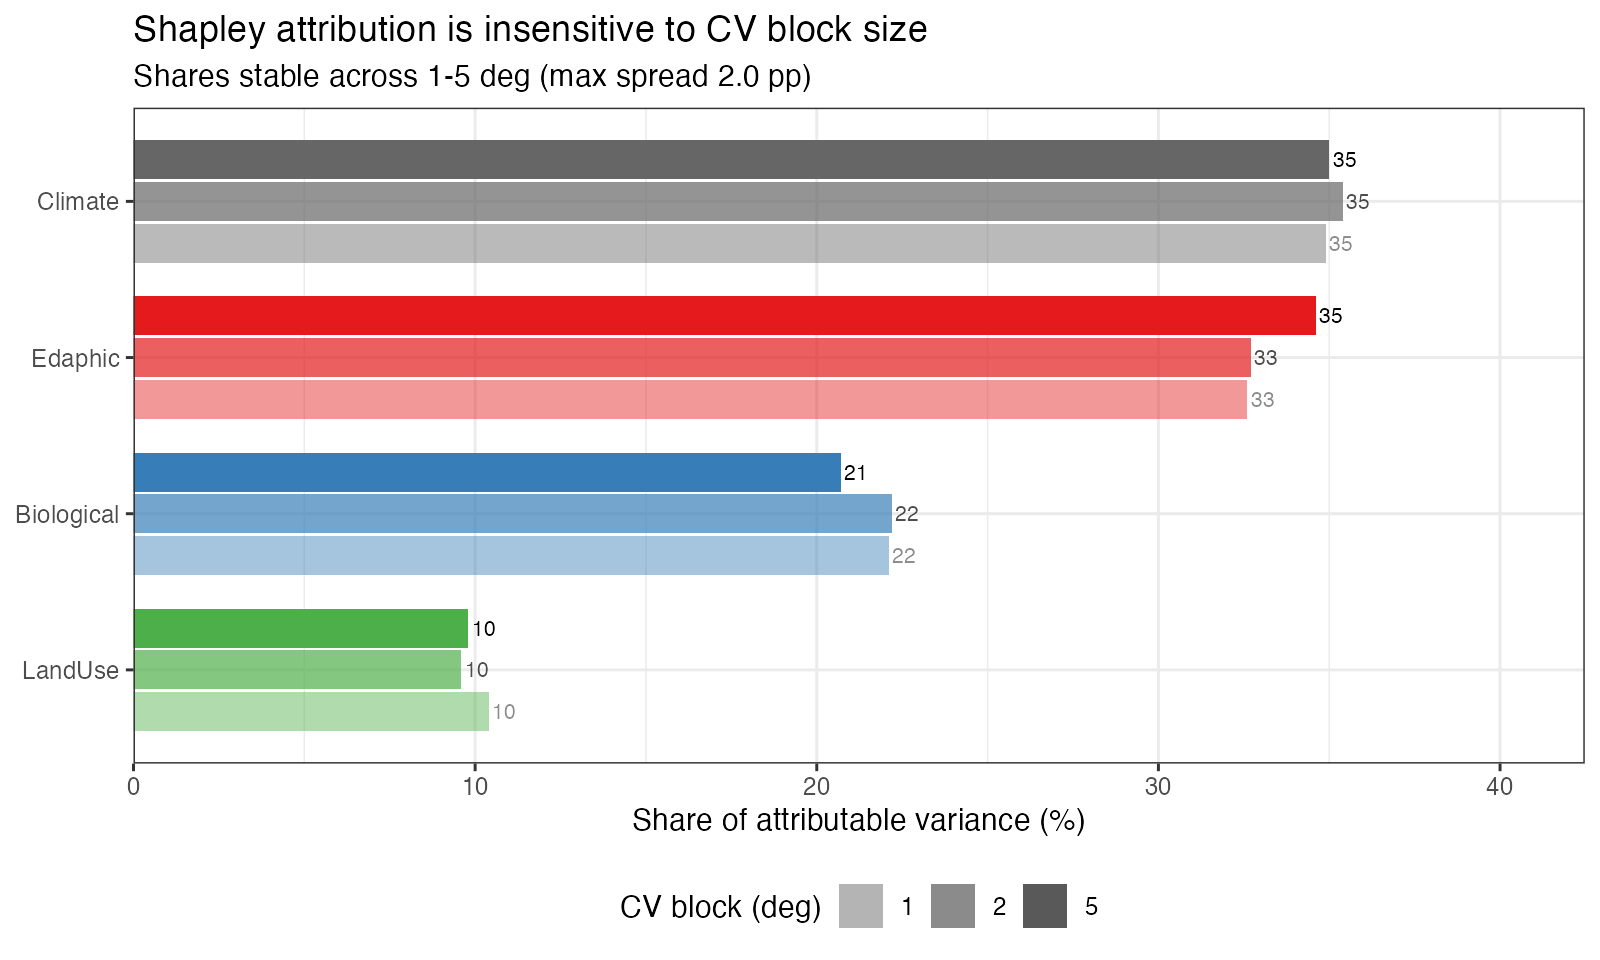
\includegraphics[width=0.8\textwidth]{../plots/step_13c_commonality/13h_blocksize_shapley.png}
\caption{\textbf{Block-size invariance.} Shapley shares across 1/2/5\textdegree{} CV blocks; maximum spread $\le$2~pp.}
\label{fig:blocksize}
\end{figure}

\begin{figure}[H]\centering
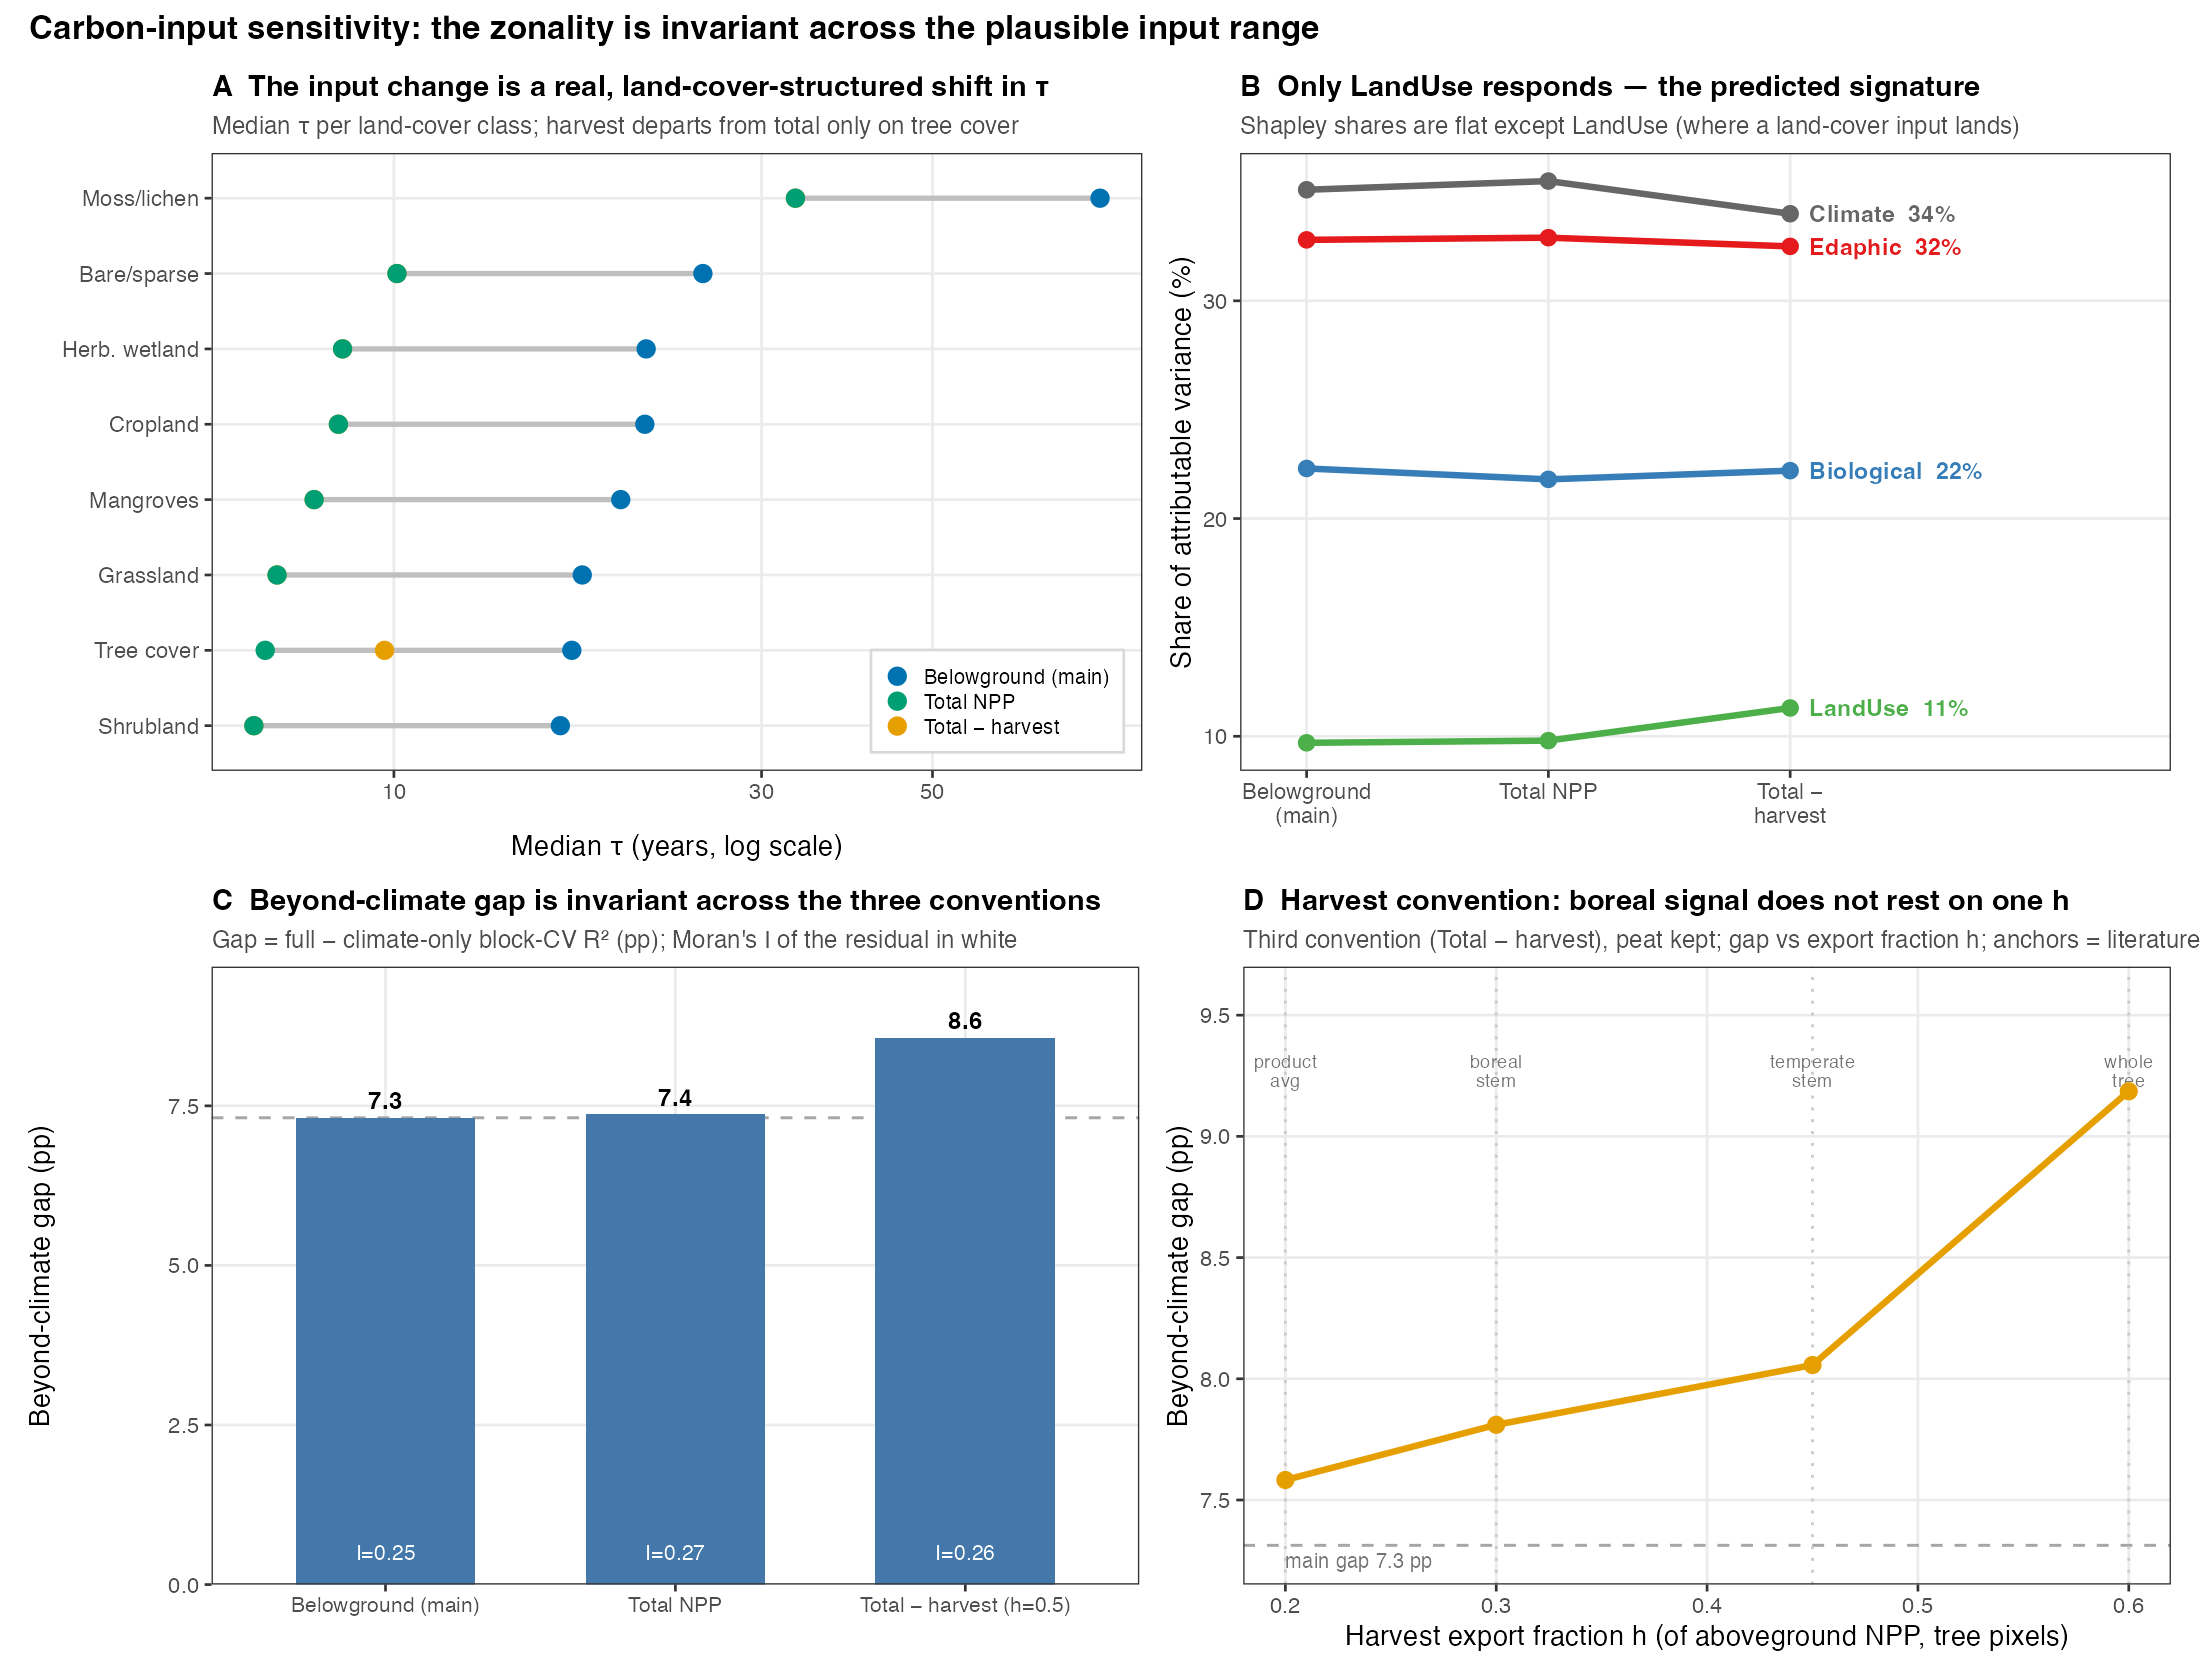
\includegraphics[width=\textwidth]{../plots/step_13c_commonality/13k_input_sensitivity_appendix.png}
\caption{\textbf{Carbon-input sensitivity.} The soil-carbon-input coefficient is
re-derived on the same NPP field under three conventions.
\textbf{(A)}~Median $\tau$ per land-cover class: the change is a real,
land-cover-structured shift in $\tau$ (harvest departs from total only on tree
cover). \textbf{(B)}~Shapley shares are flat across conventions except LandUse, the
axis a land-cover-structured coefficient projects onto. \textbf{(C)}~The
beyond-climate gap (full minus climate-only block-CV $R^2$; Moran's $I$ of the
residual inset) is invariant across conventions. \textbf{(D)}~For the harvest
convention, the gap does not fall as the export fraction $h$ is swept across its
literature range (product-average, boreal and temperate stem-only, whole-tree).}
\label{fig:input_sensitivity}
\end{figure}

\begin{figure}[H]\centering
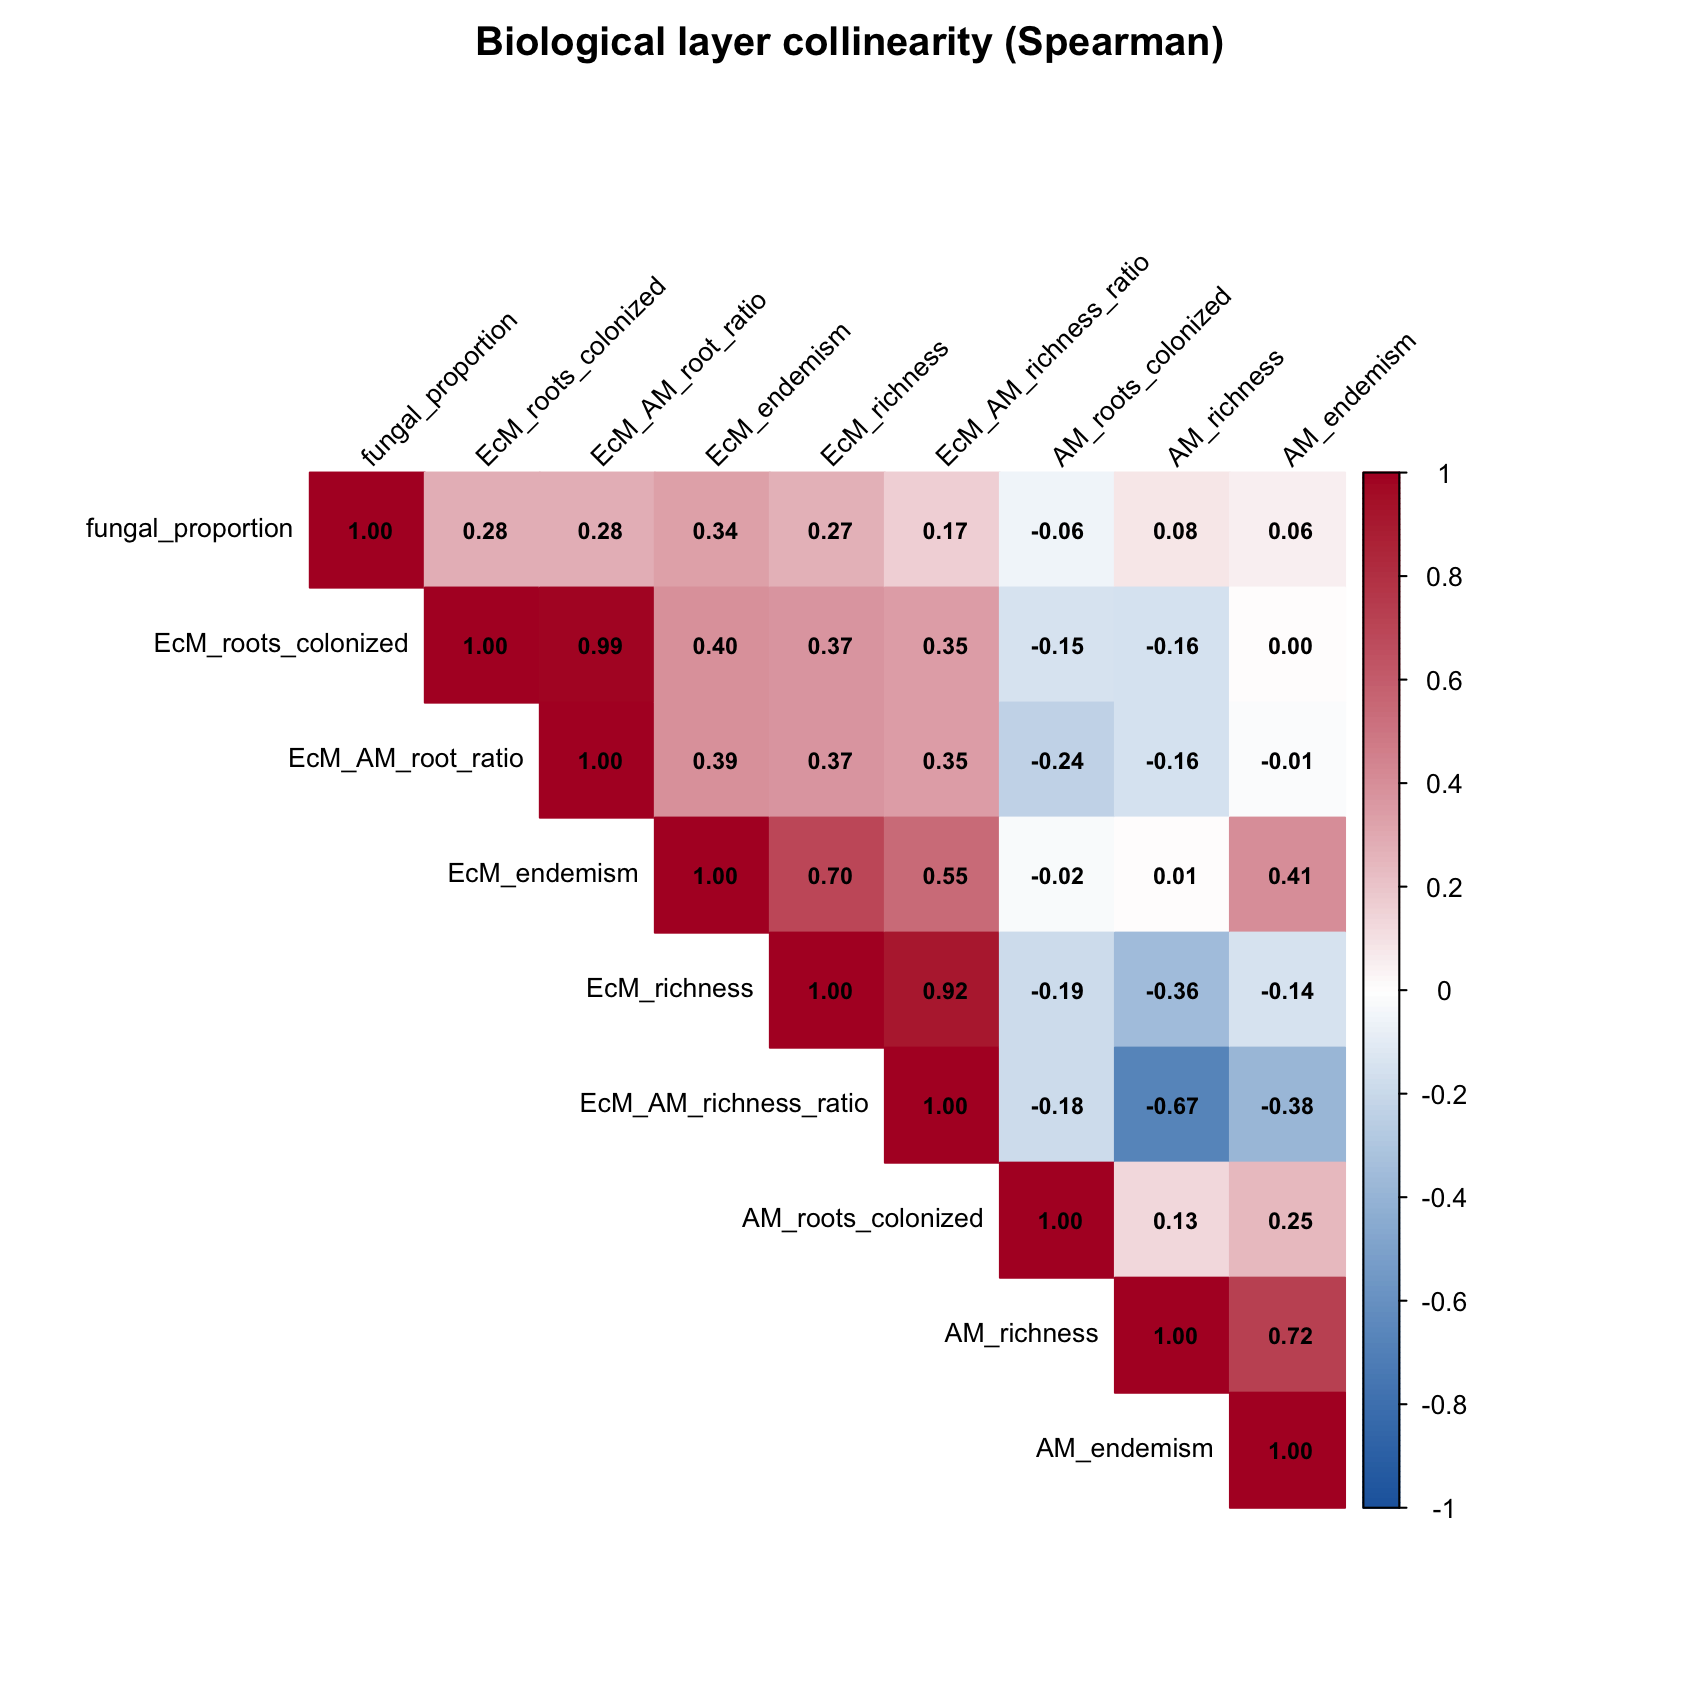
\includegraphics[width=0.95\textwidth]{../plots/appendix/biological_collinearity.png}
\caption{\textbf{Biological parsimony.} Collinearity among the nine biological layers and single-layer skill vs coverage, justifying the default six-layer set; the three root-colonisation layers add negligible unique skill. See also \texttt{biological\_single\_layer\_skill}.}
\label{fig:parsimony}
\end{figure}

\begin{figure}[H]\centering
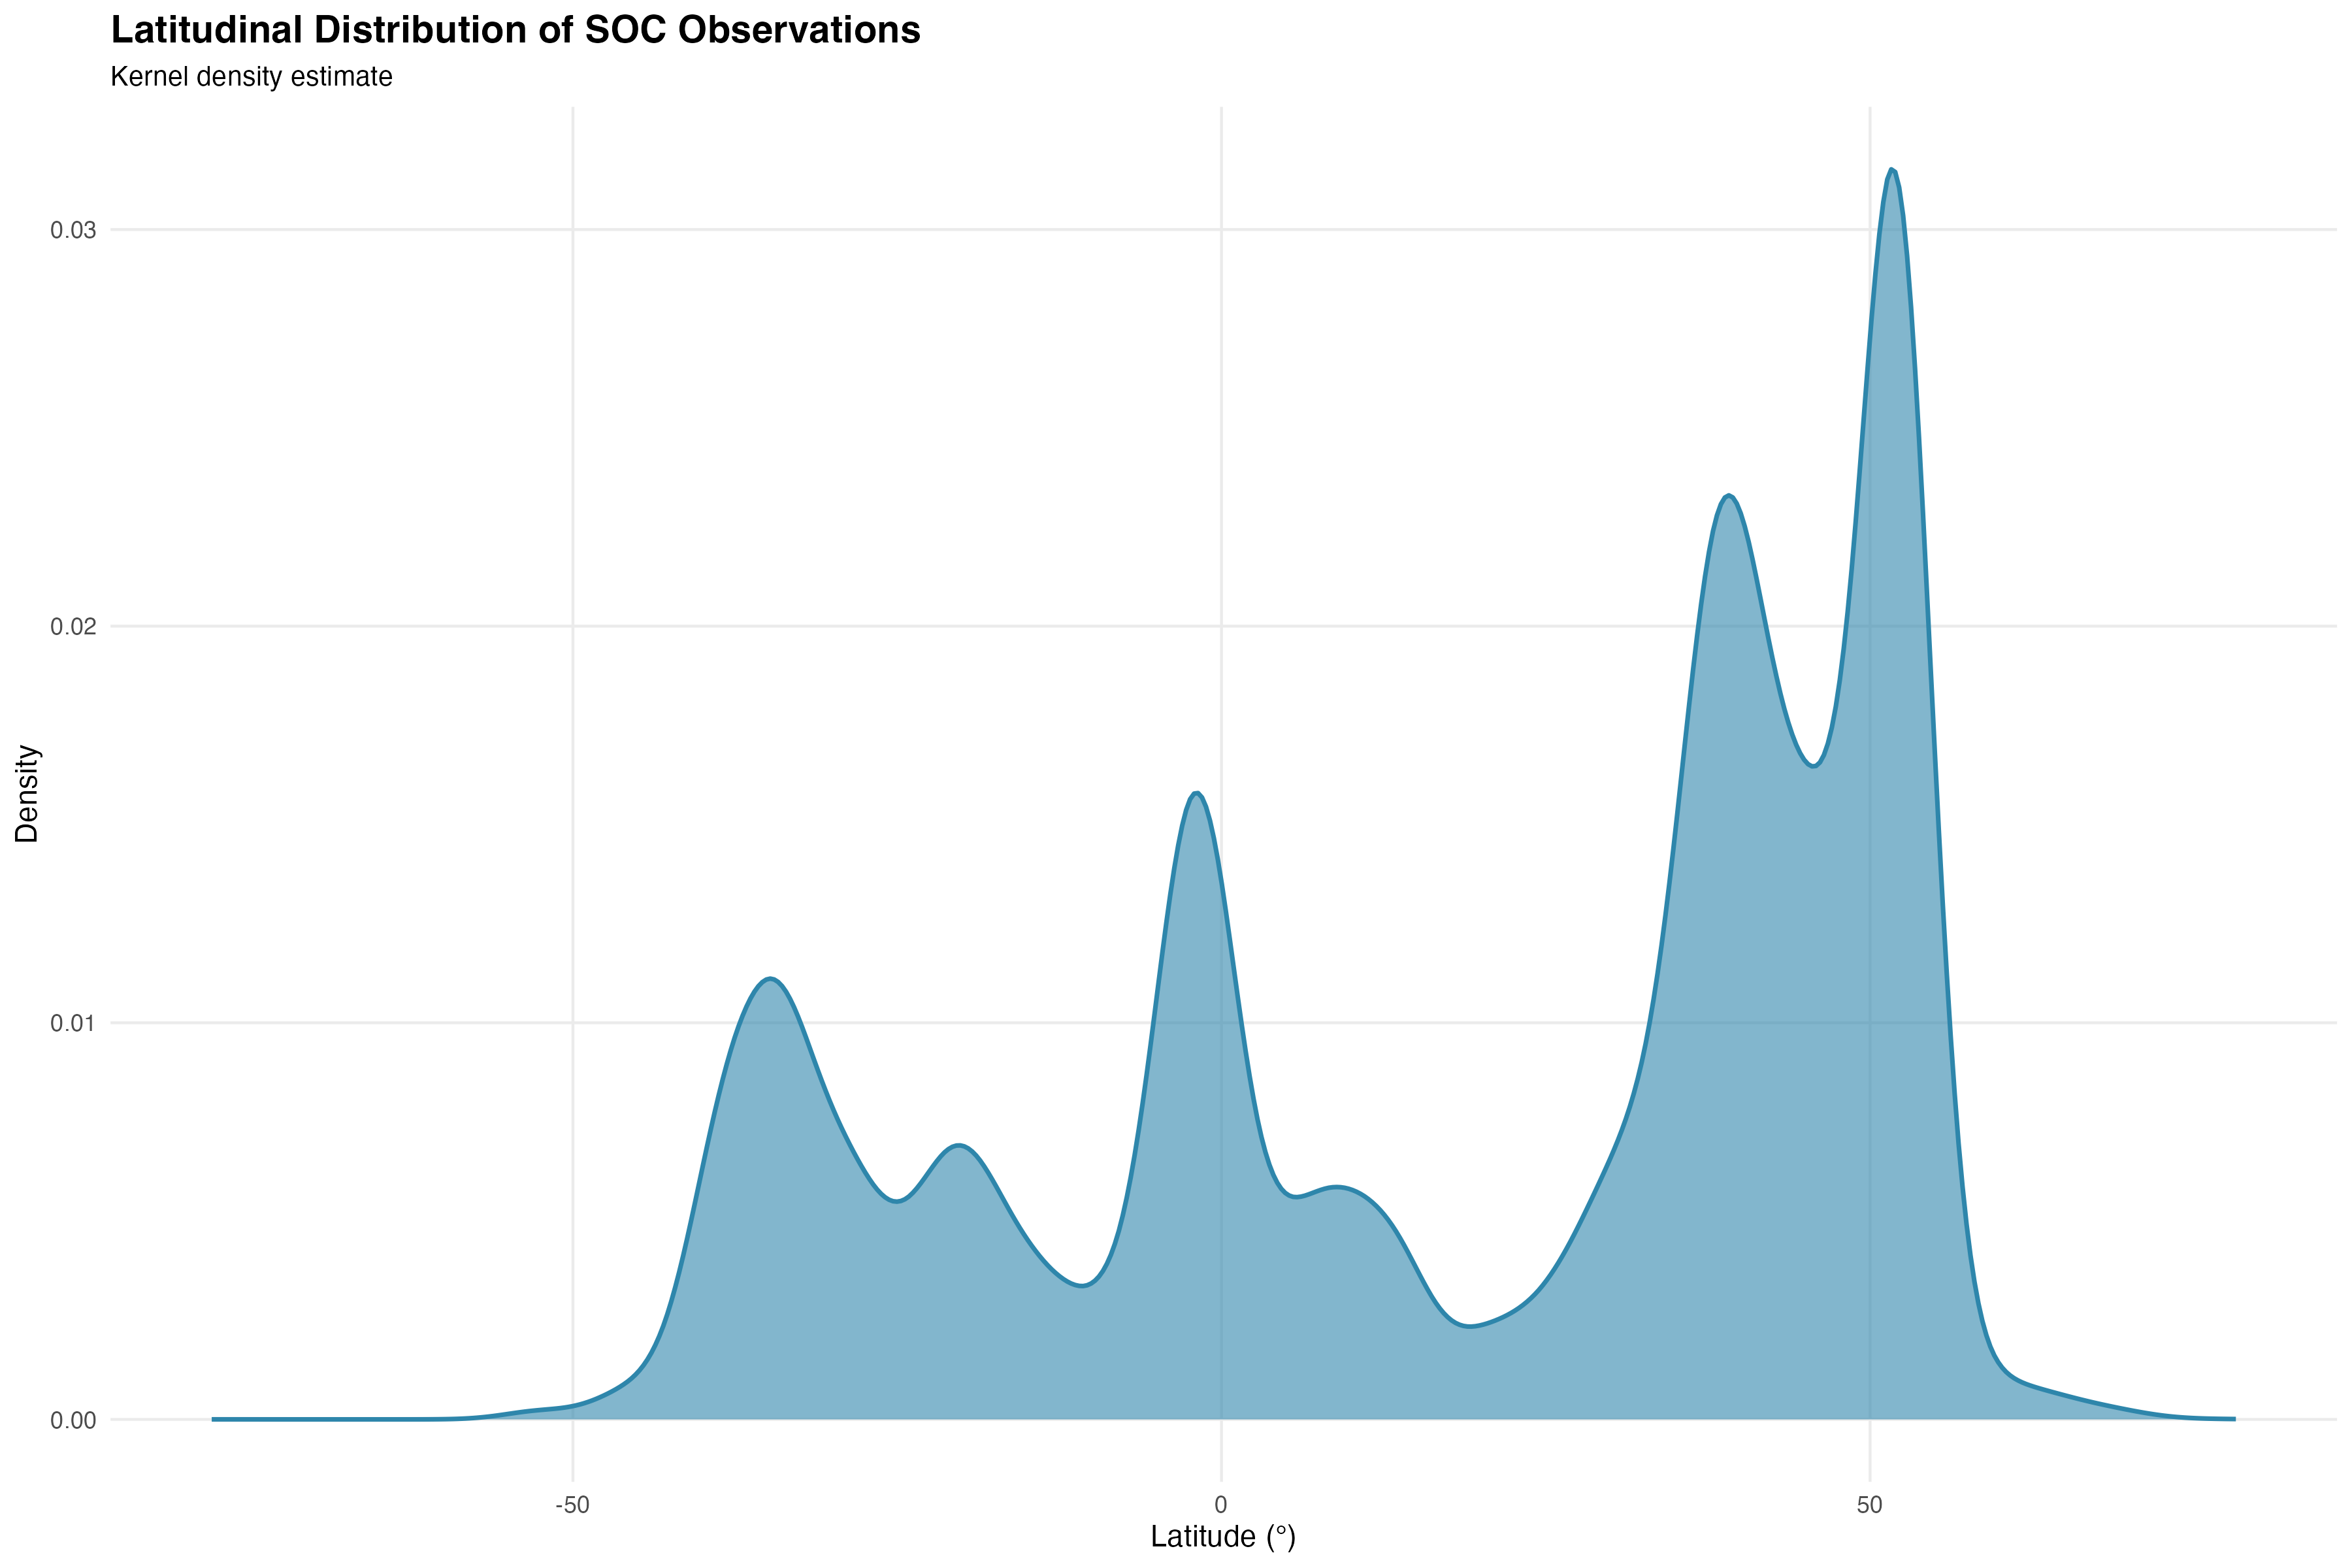
\includegraphics[width=0.95\textwidth]{../plots/step_17_visualizations/latitudinal_sampling_coverage.png}
\caption{\textbf{Latitudinal sampling coverage.} Density of the OpenLandMap soil profiles used for training, by latitude.}
\label{fig:sampling}
\end{figure}

\begin{figure}[H]\centering
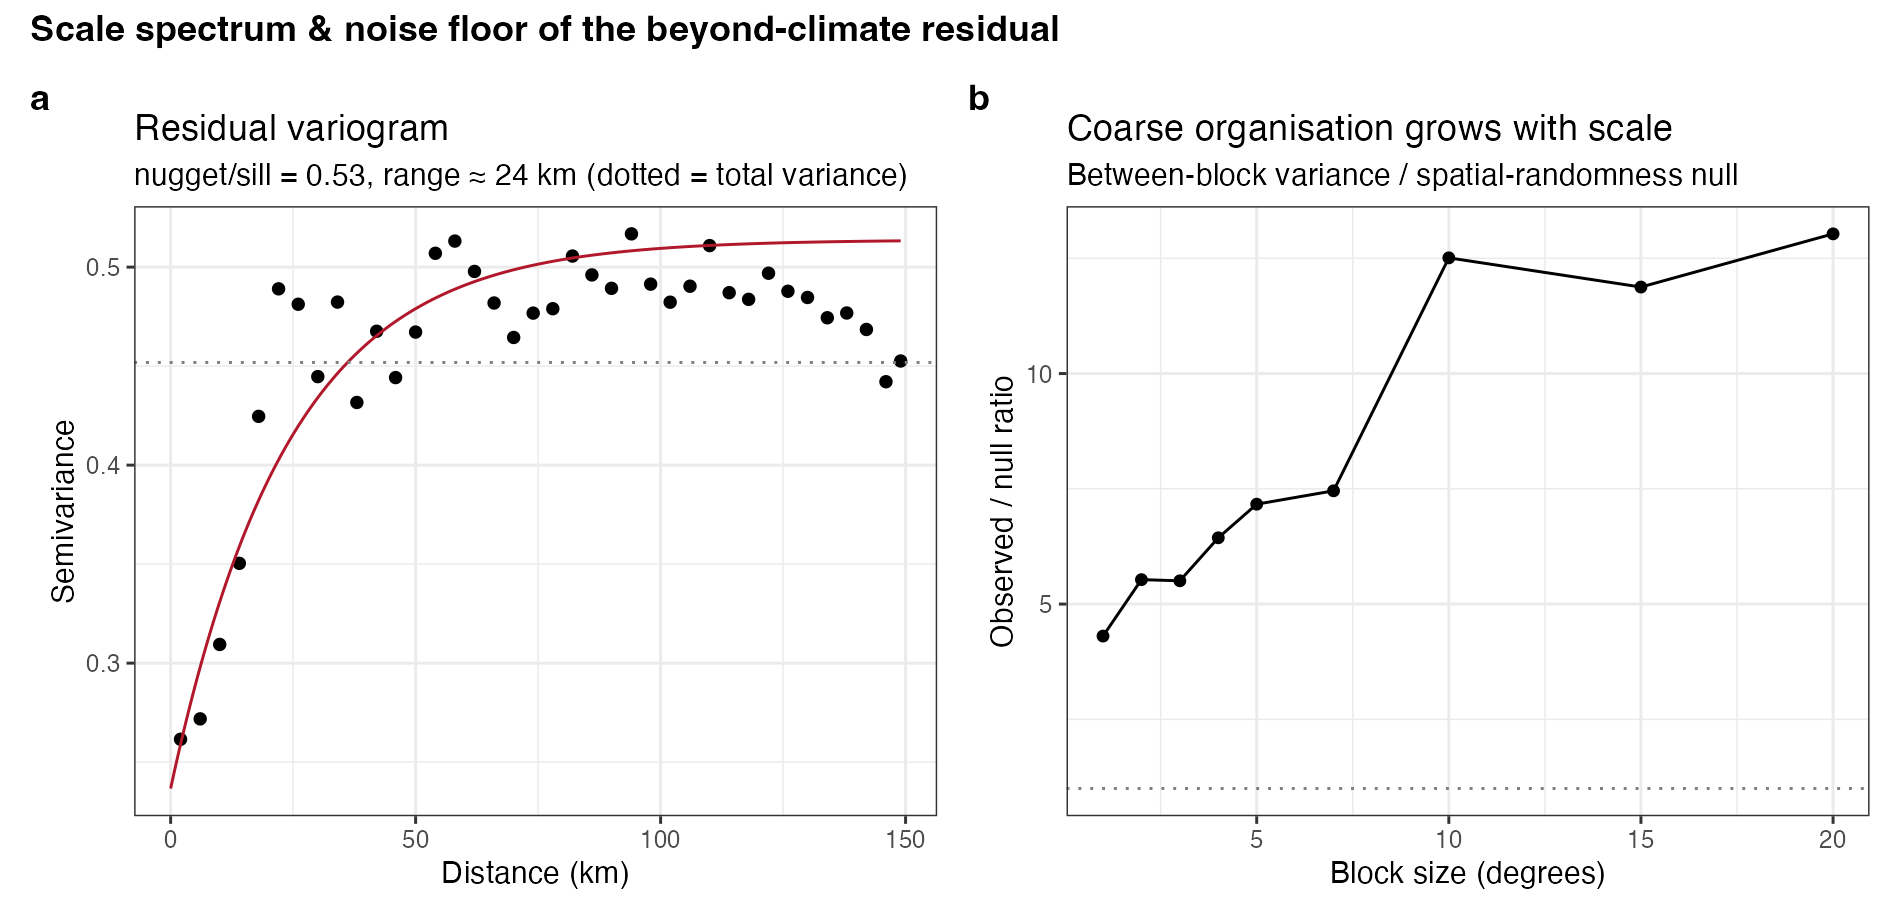
\includegraphics[width=0.95\textwidth]{../plots/appendix/scale_noisefloor.png}
\caption{\textbf{Scale spectrum and noise floor.} (a)~Residual variogram (nugget/sill~$\approx$0.56, range~$\approx$16~km); (b)~coarse organisation grows with block size.}
\label{fig:noisefloor}
\end{figure}

\begin{figure}[H]\centering
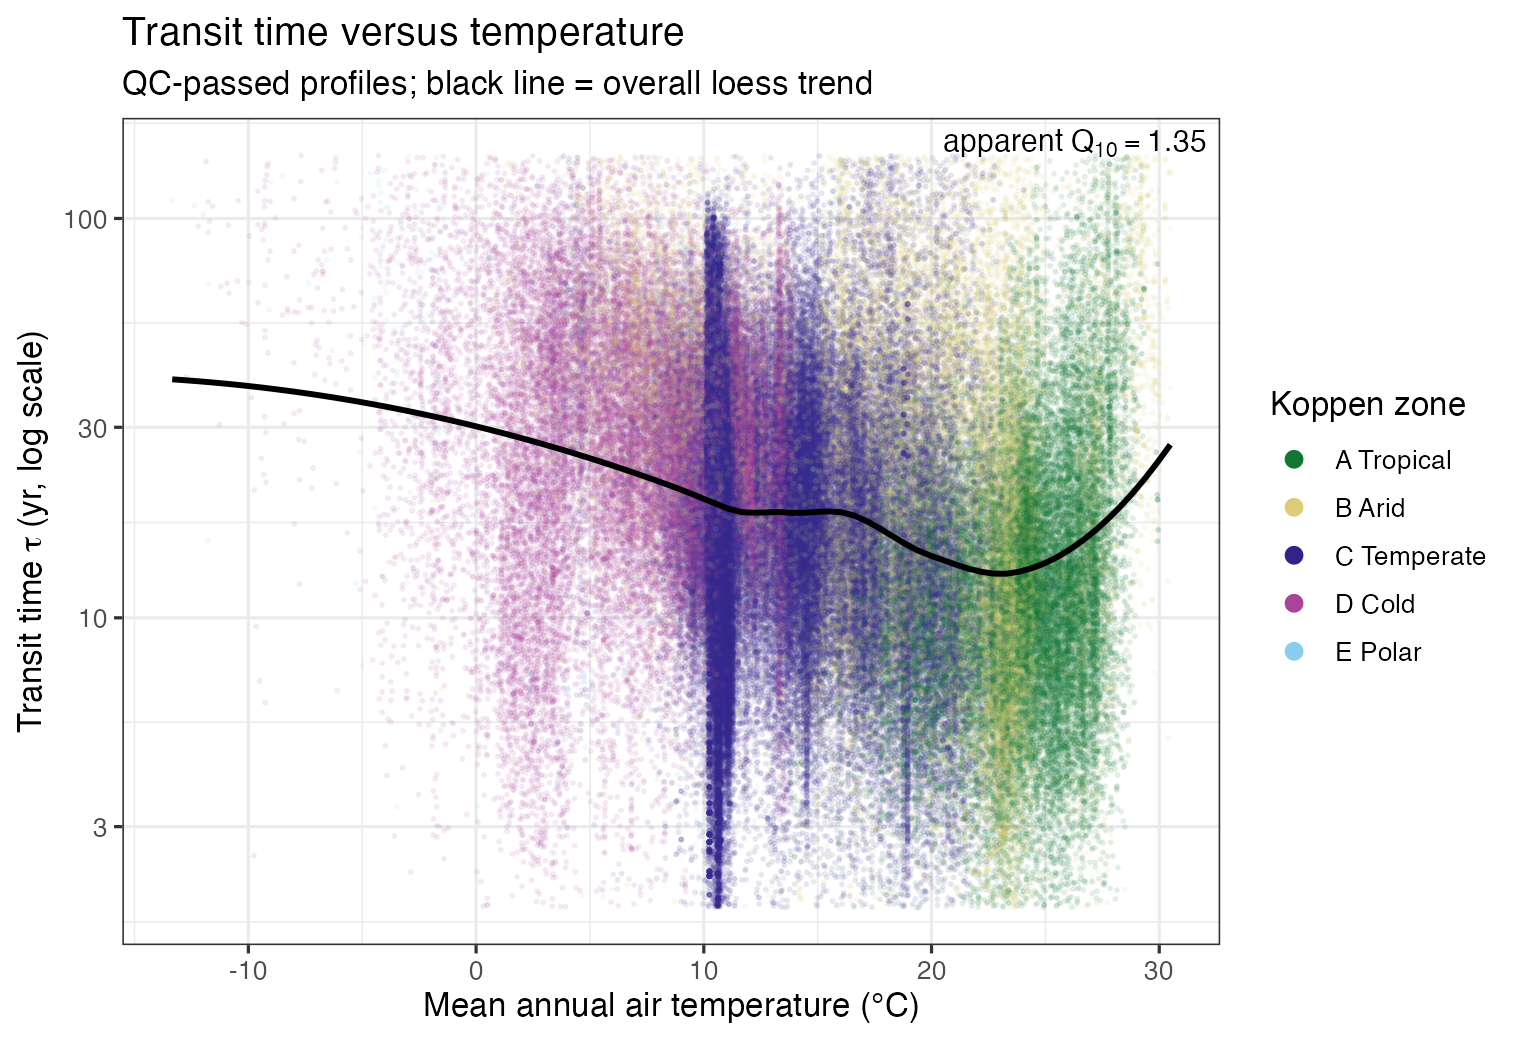
\includegraphics[width=0.8\textwidth]{../plots/appendix/22_temperature_tau_scatter.png}
\caption{\textbf{Transit time versus temperature.} Observed $\tau$ (log scale) against mean annual air temperature for the QC-passed profiles, coloured by coarse K\"oppen zone, with an overall loess trend (black). Transit time declines with warming, from ${\sim}35$~yr in the coldest soils to a minimum of ${\sim}13$~yr near 22--23\textdegree{}C, corresponding to an apparent $Q_{10}$ of bulk turnover of about 1.35 (log-linear fit, $R^2=0.06$). The upturn at the warmest end is consistent with the U-shaped soil-temperature response in Fig.~\ref{fig:ale_top10} (hot, dry soils turning over more slowly). This single-predictor view is shown for comparability with earlier compilations \citep[e.g.][]{Varney2020}; the weak fit ($R^2=0.06$) underscores that temperature alone explains little of the point-level variation in $\tau$.}
\label{fig:tempscatter}
\end{figure}

\begin{figure}[H]\centering
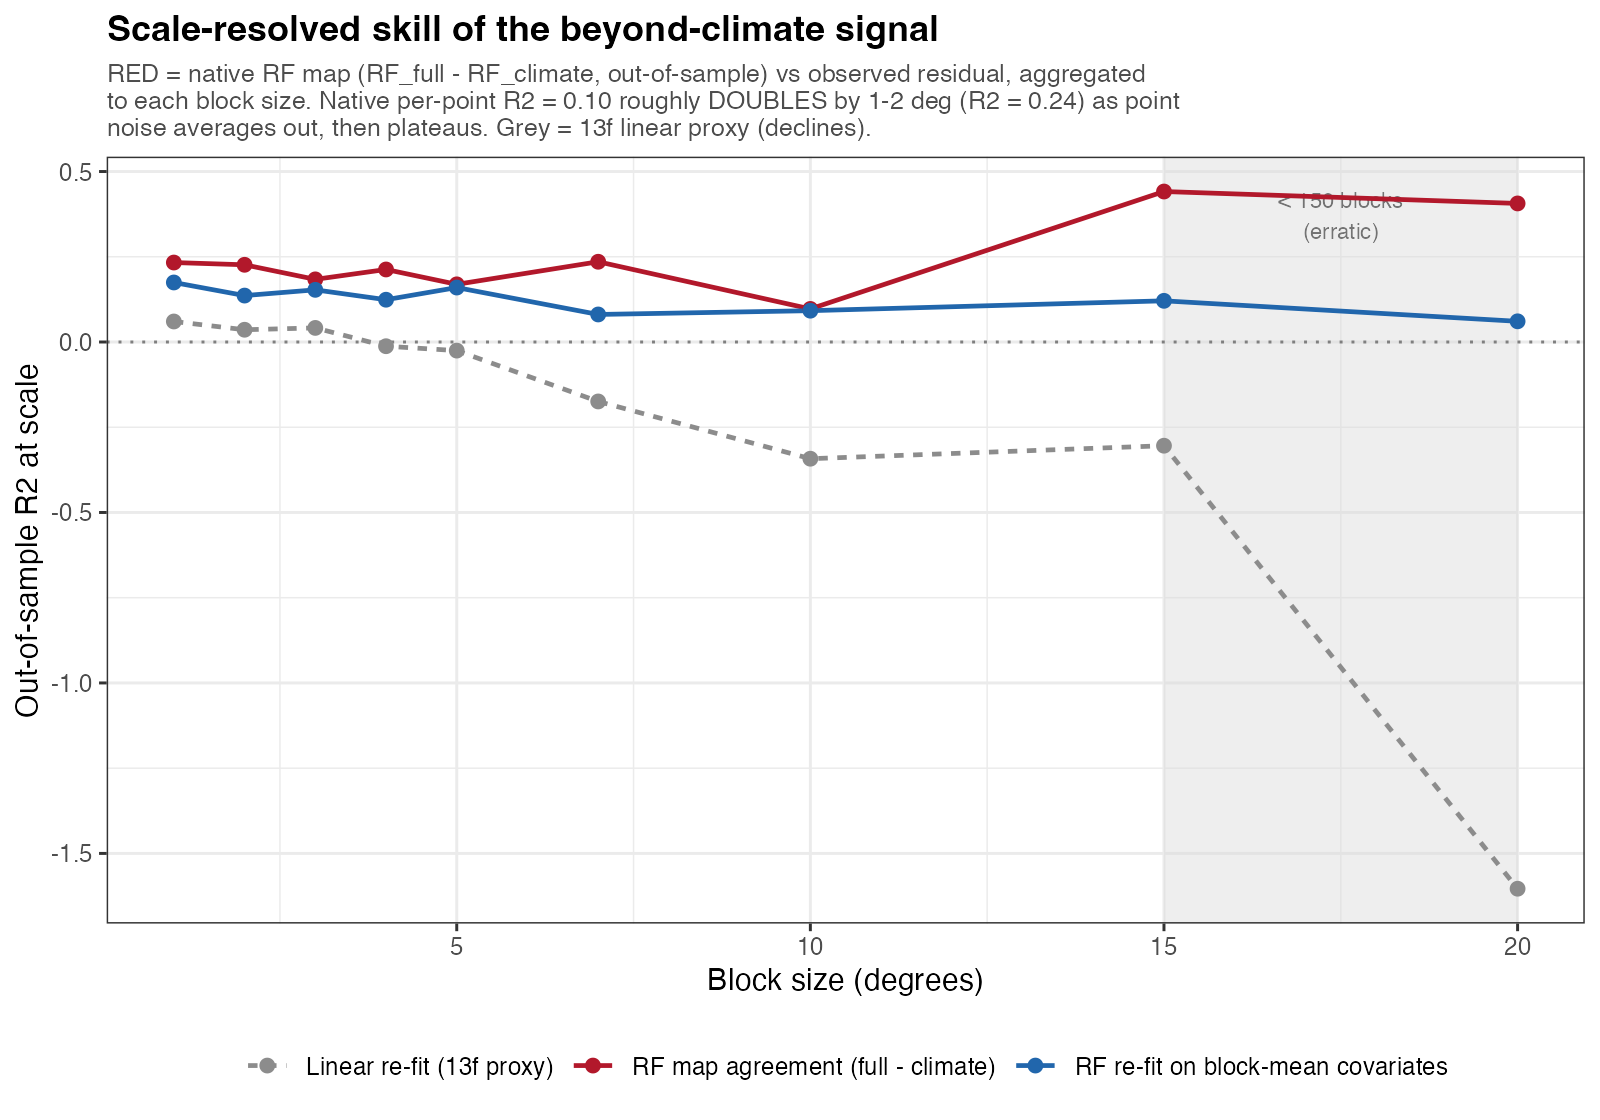
\includegraphics[width=0.85\textwidth]{../plots/appendix/scale_rf_mapping_skill.png}
\caption{\textbf{RF mapping skill vs scale.} Agreement of the native beyond-climate map with the observed residual when aggregated to each block size: $R^2\approx0.11$ native, $\approx0.22$ by 1--2\textdegree, plateau across 1--7\textdegree; the linear proxy (grey) declines.}
\label{fig:mapskill}
\end{figure}

\begin{figure}[H]\centering
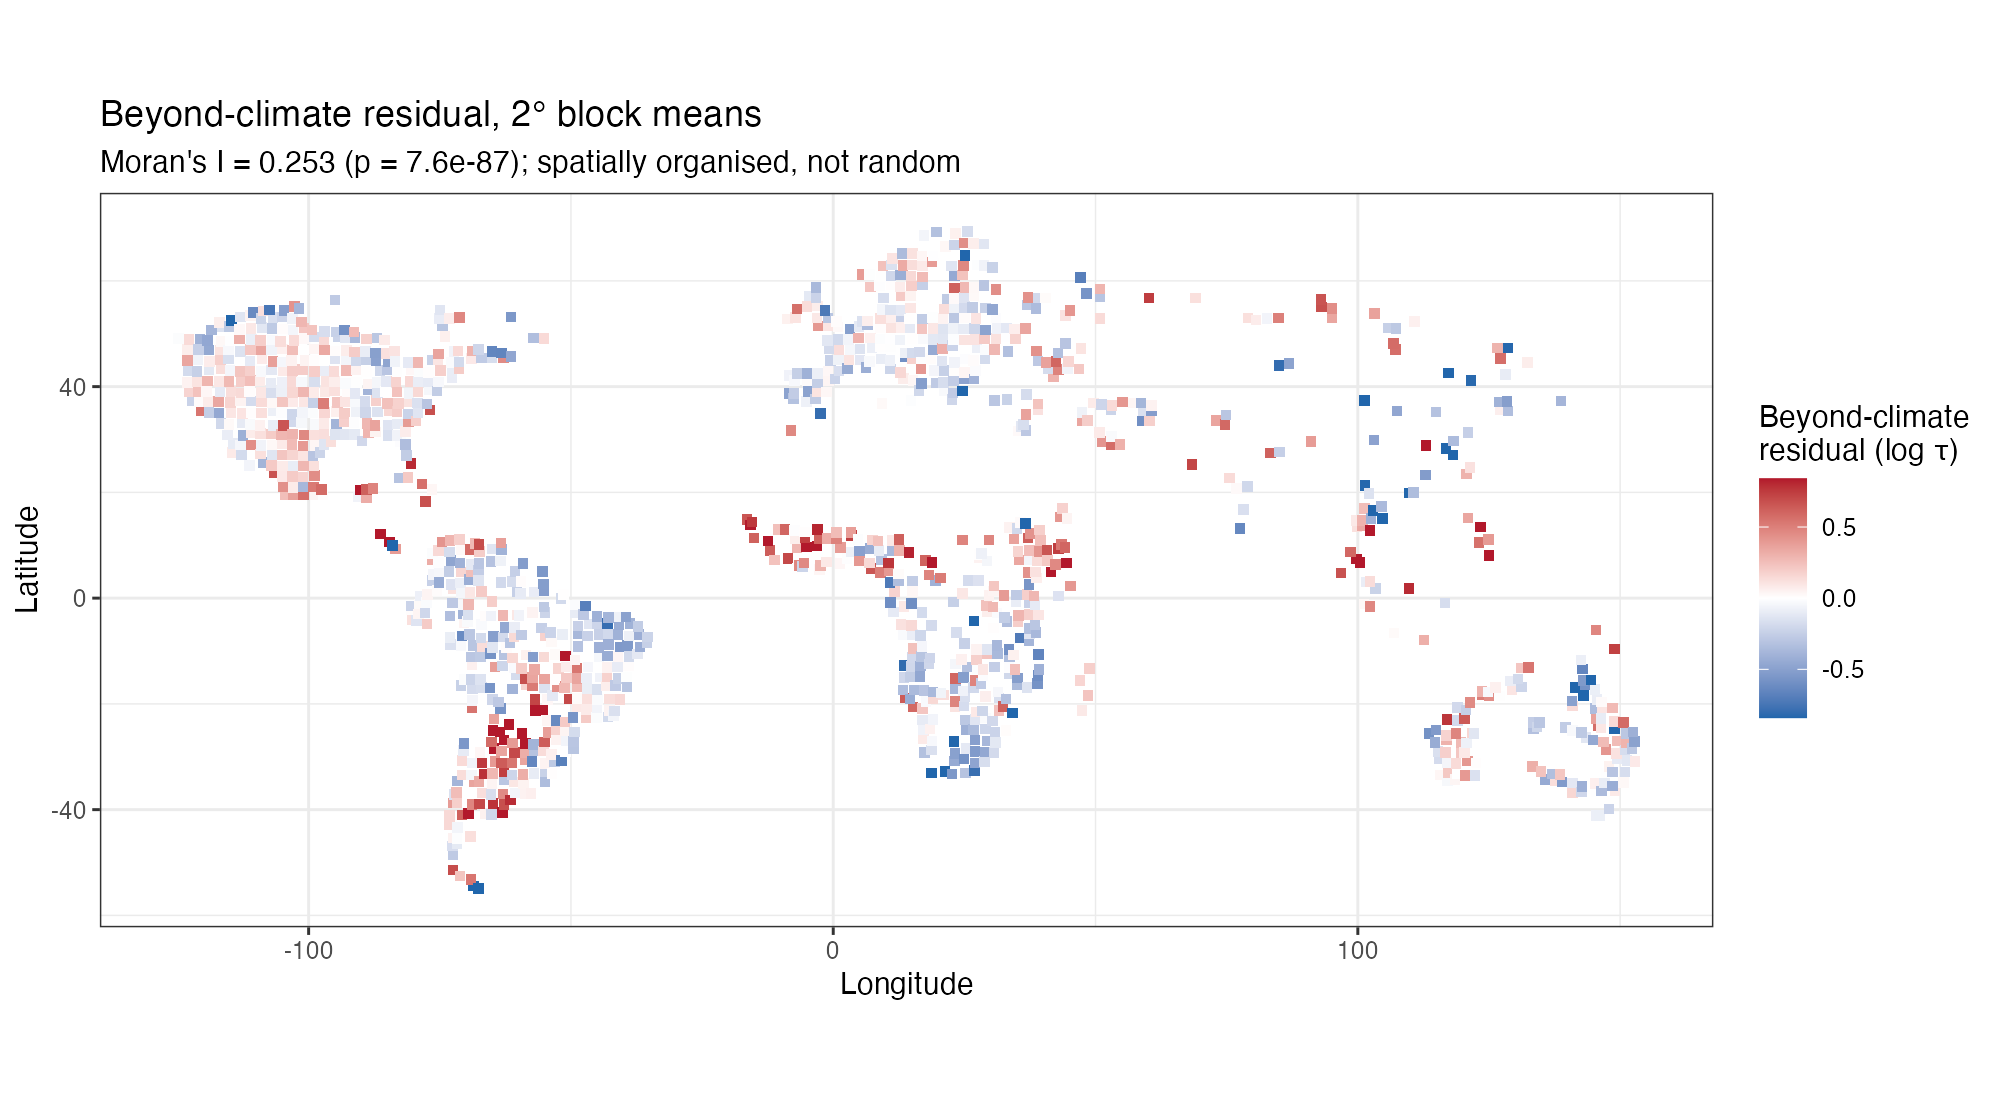
\includegraphics[width=0.85\textwidth]{../plots/step_13c_commonality/13e_block_residual_map.png}
\caption{\textbf{Tier-1 residual map.} Block-mean beyond-climate residual; the organised companion to the Moran scatter.}
\label{fig:residmap}
\end{figure}

\begin{figure}[H]\centering
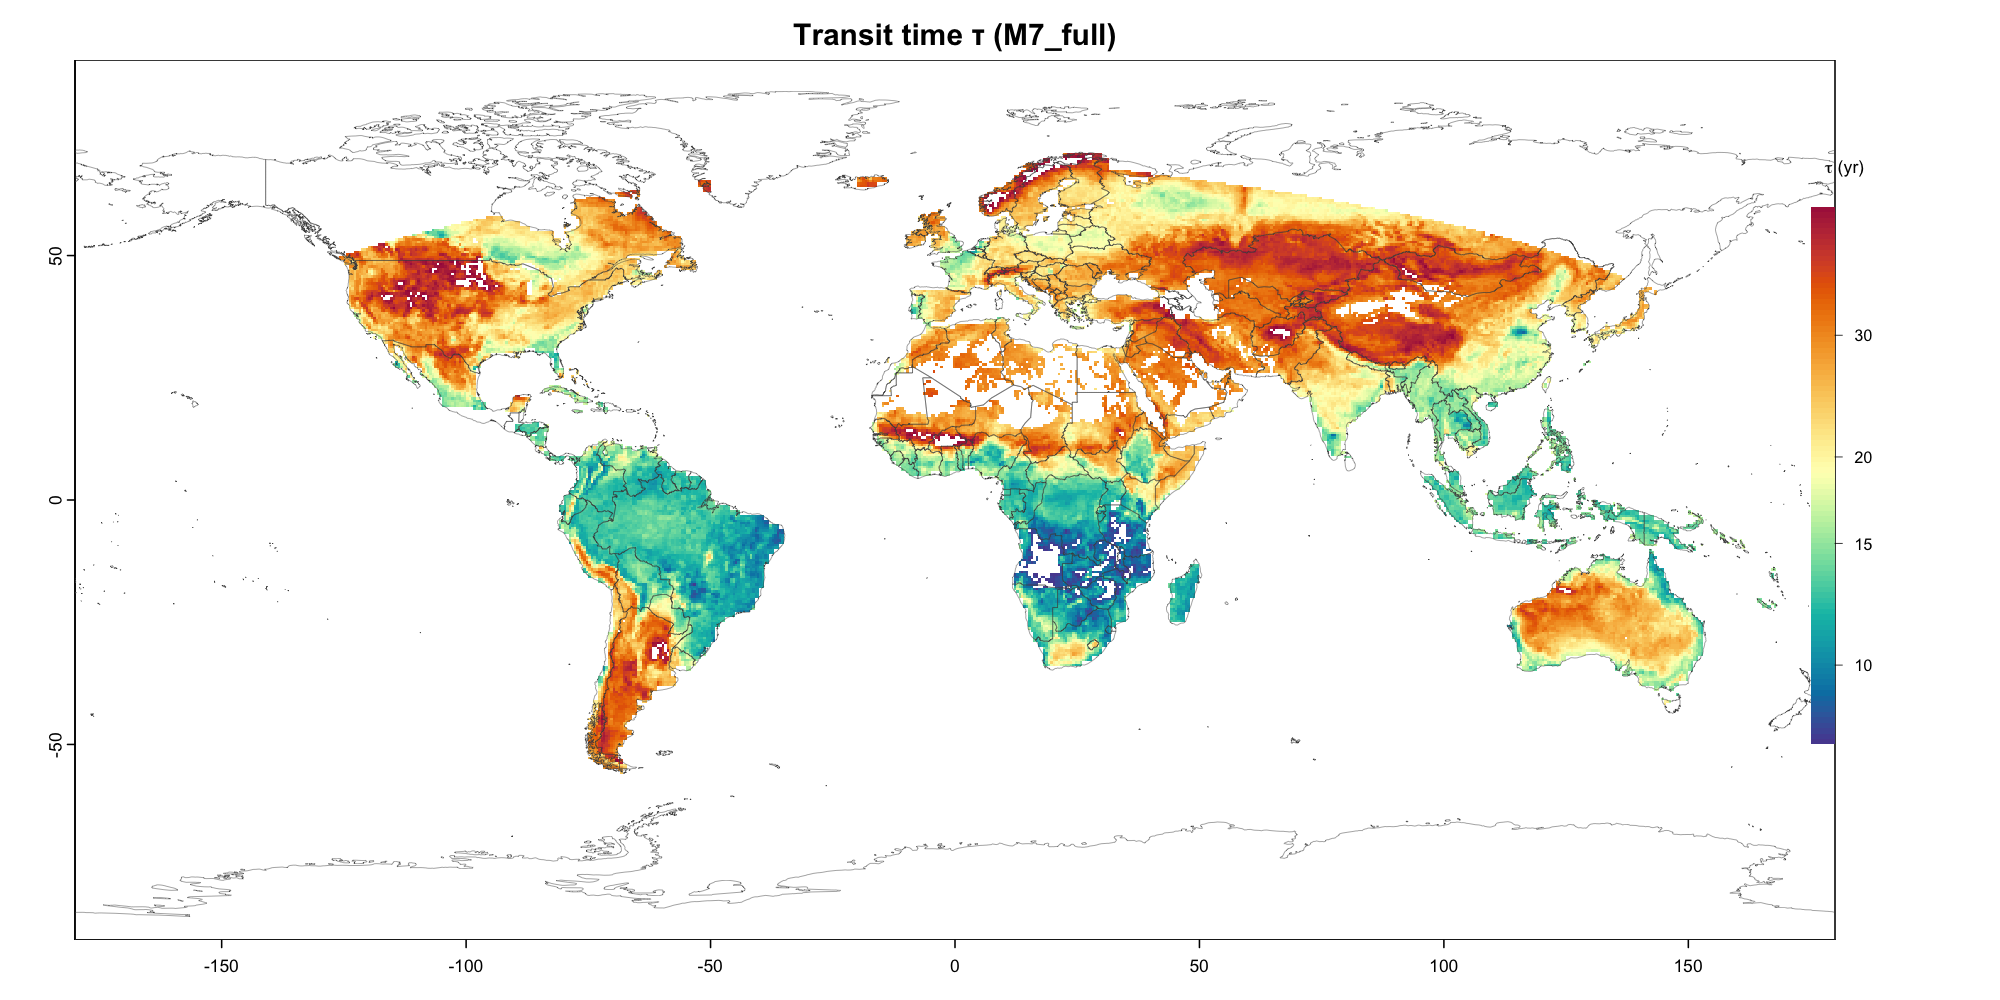
\includegraphics[width=1.0\textwidth]{../plots/step_17_visualizations/MRT_M7_full_map_log.png}
\caption{\textbf{Global distribution of predicted SOC mean transit time ($\tau$).} Full-model prediction at 0.1\textdegree{}, log-scale palette; ticks in years.}
\label{fig:global_mrt}
\end{figure}

\begin{figure}[H]\centering
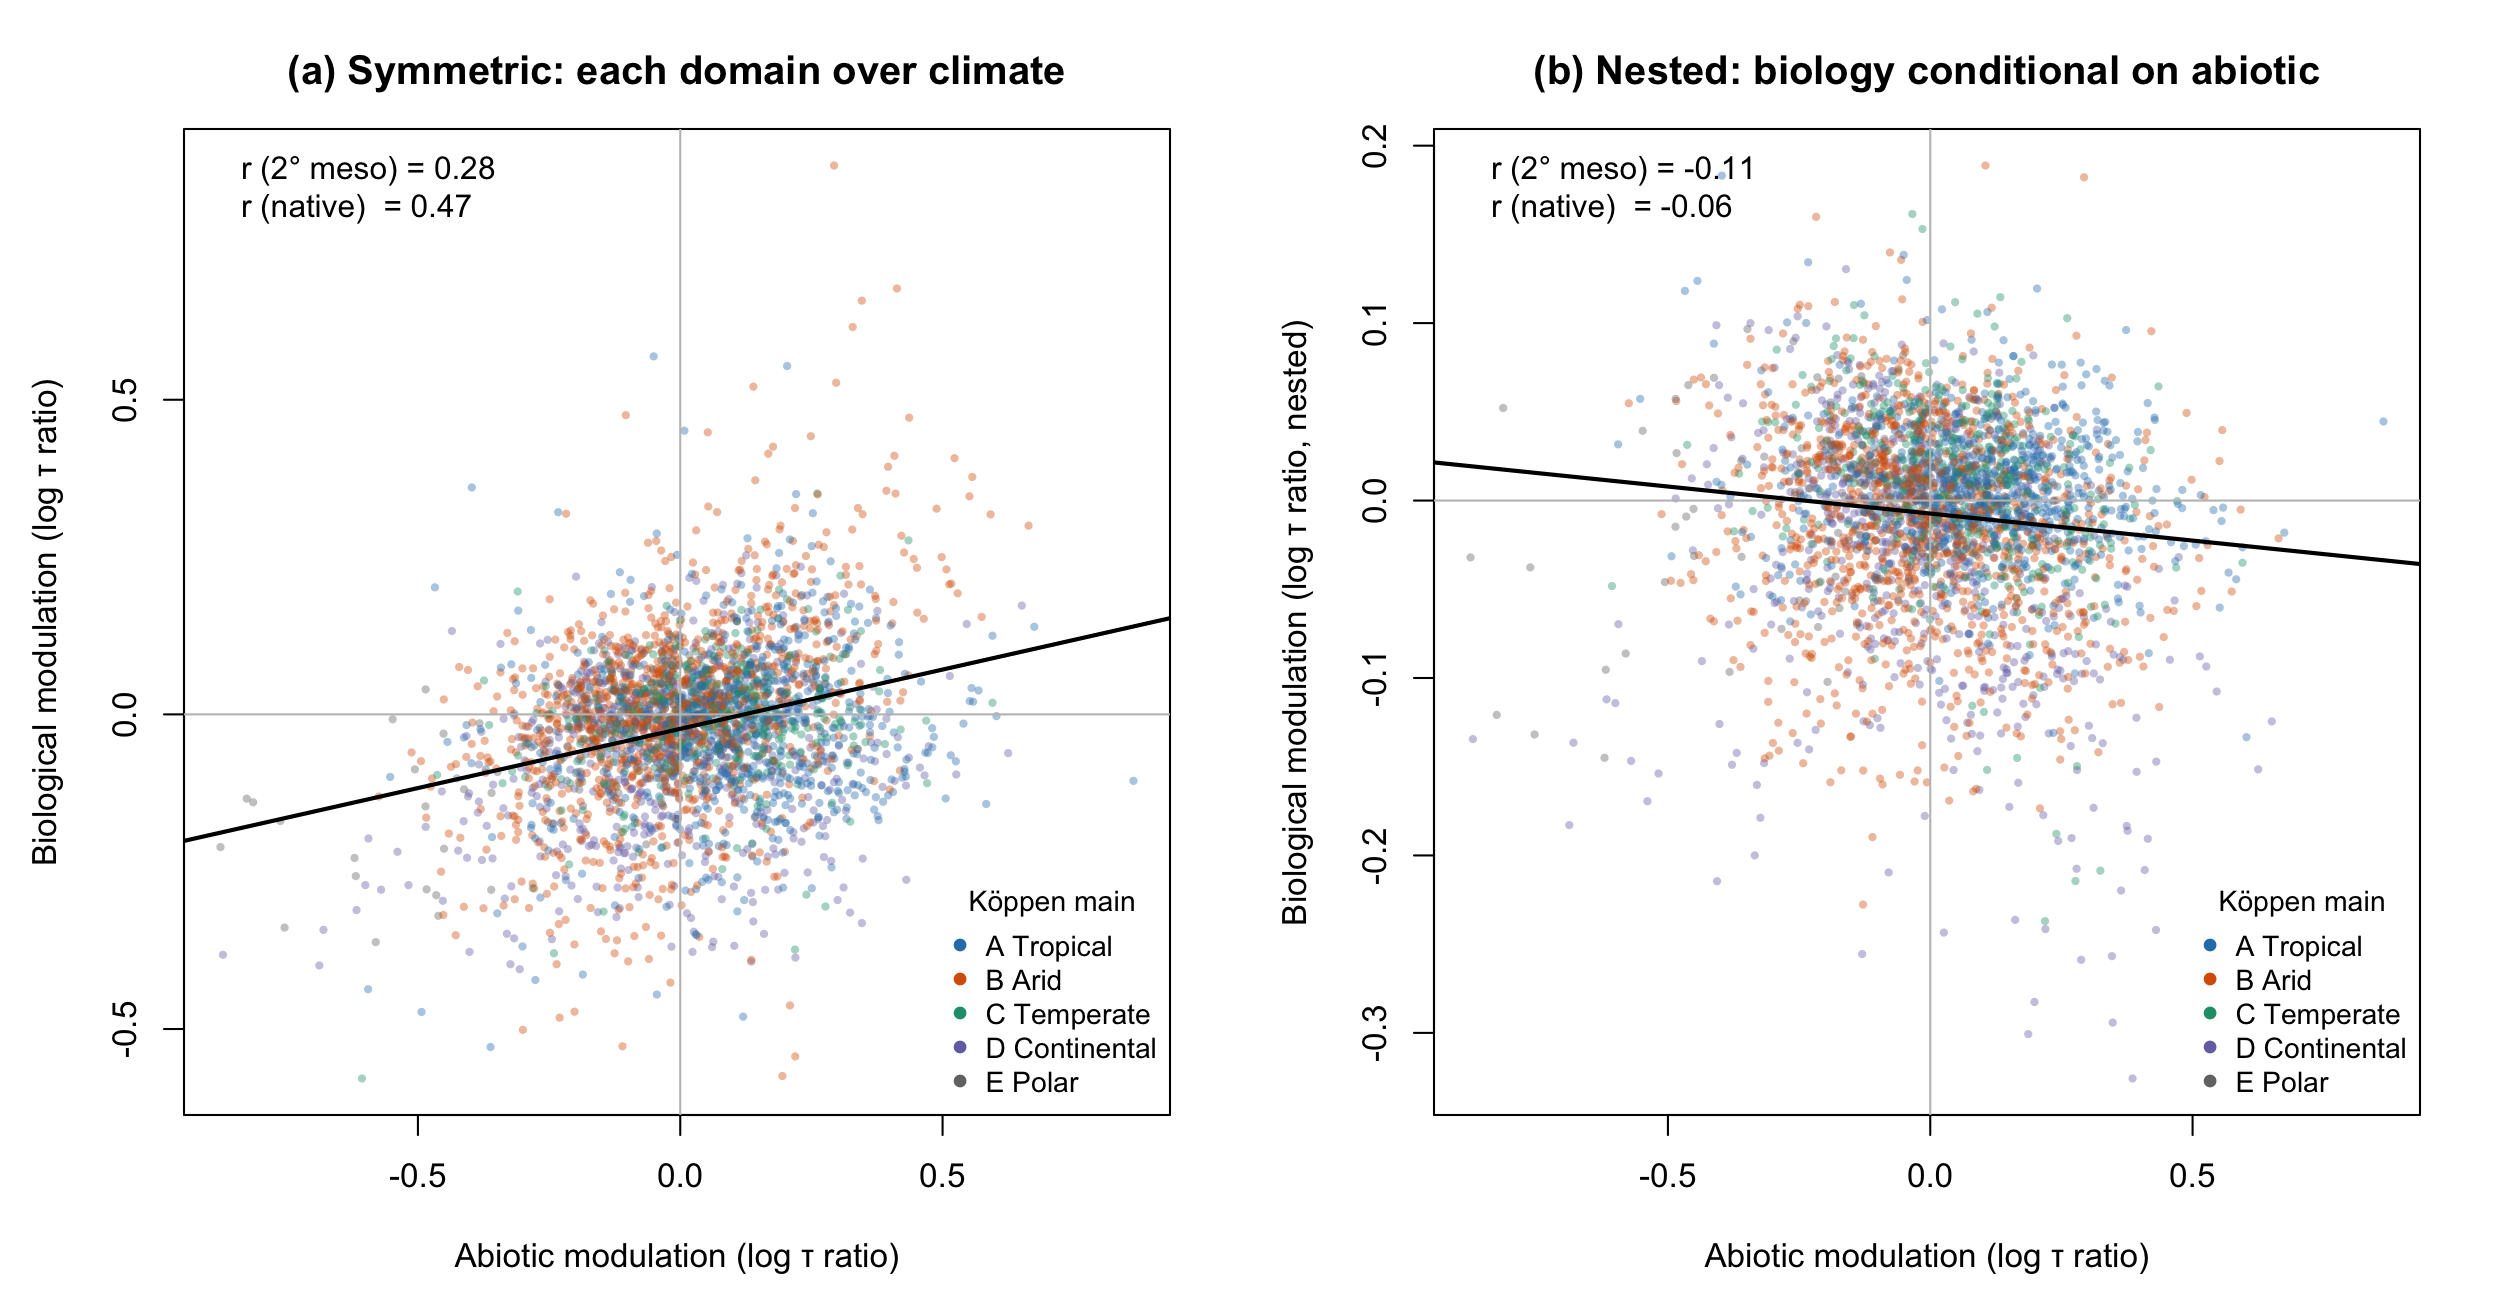
\includegraphics[width=0.72\textwidth]{../plots/step_15b_zonality/zonality_modulation_scatter.png}
\caption{\textbf{Abiotic vs biological modulation} (K\"oppen-coloured): symmetric pair co-varies ($r\approx0.4$--0.5), nested pair orthogonal ($r\approx0$).}
\label{fig:bioscatter}
\end{figure}

\begin{figure}[H]\centering
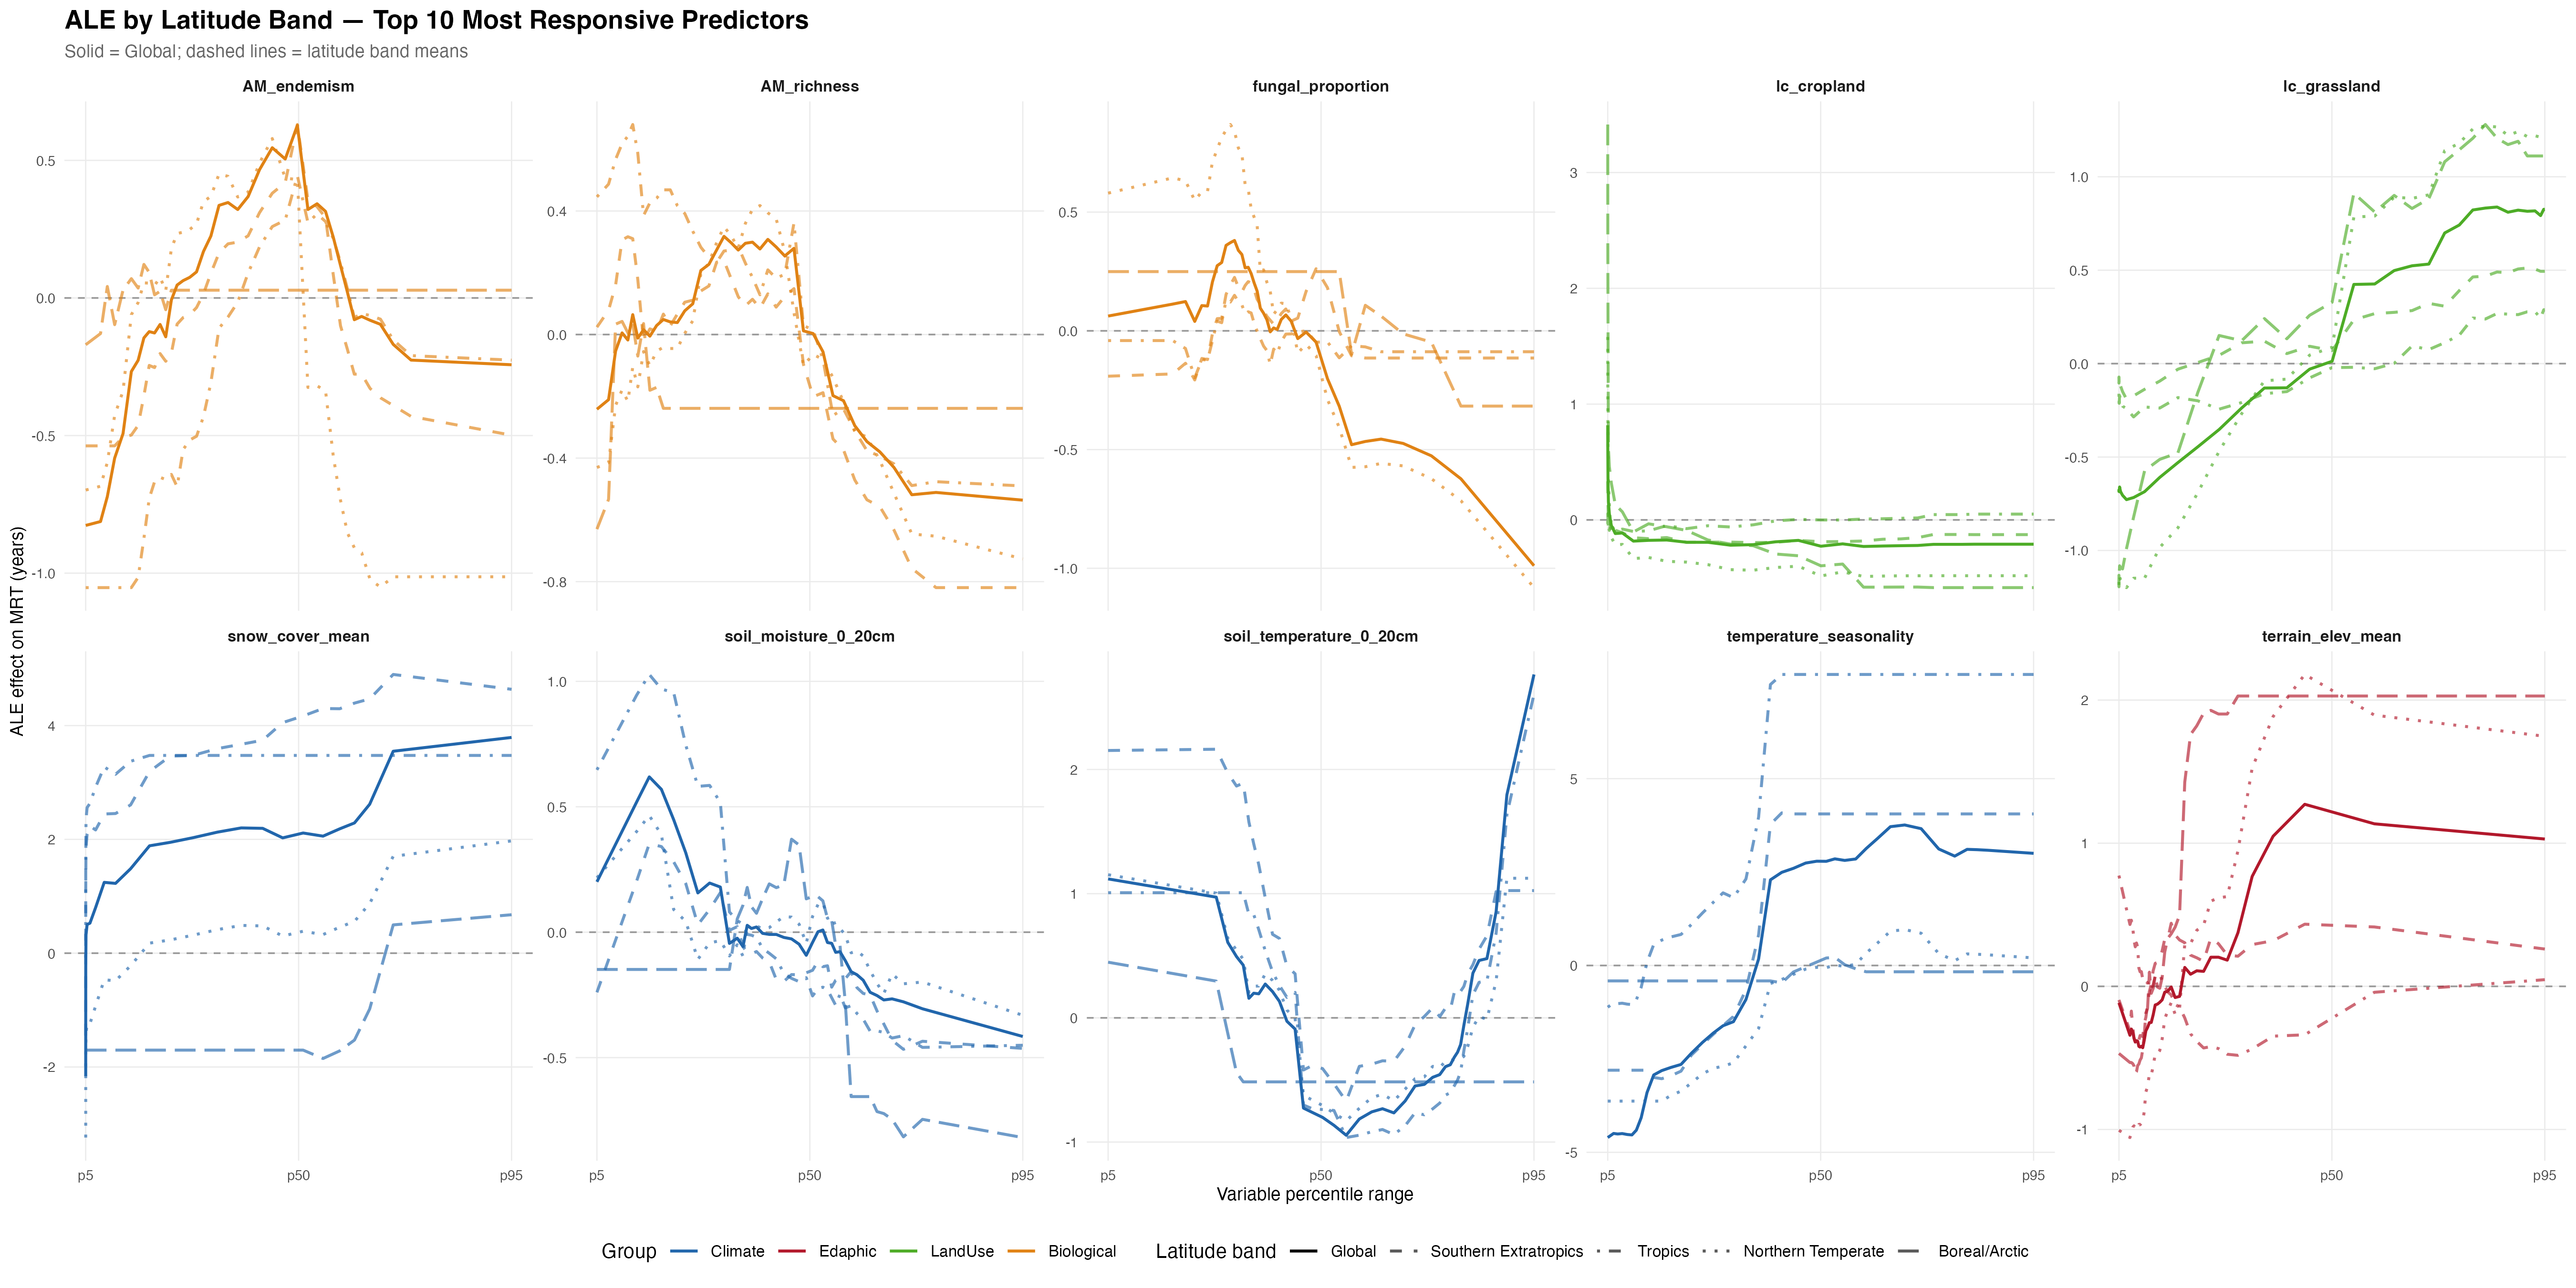
\includegraphics[width=0.95\textwidth]{../plots/step_18_sensitivity/18C_ALE_by_latband.png}
\caption{\textbf{ALE response curves by latitude band.} Marginal responses of
$\tau$ to each continuous predictor, computed globally and within four latitude
bands (southern temperate, tropics, northern temperate, boreal/Arctic). The
band-resolved curves underlie the latitude-band statements in
Sec.~\ref{sec:results_ale}.}
\label{fig:ale_latband}
\end{figure}

\begin{figure}[H]\centering
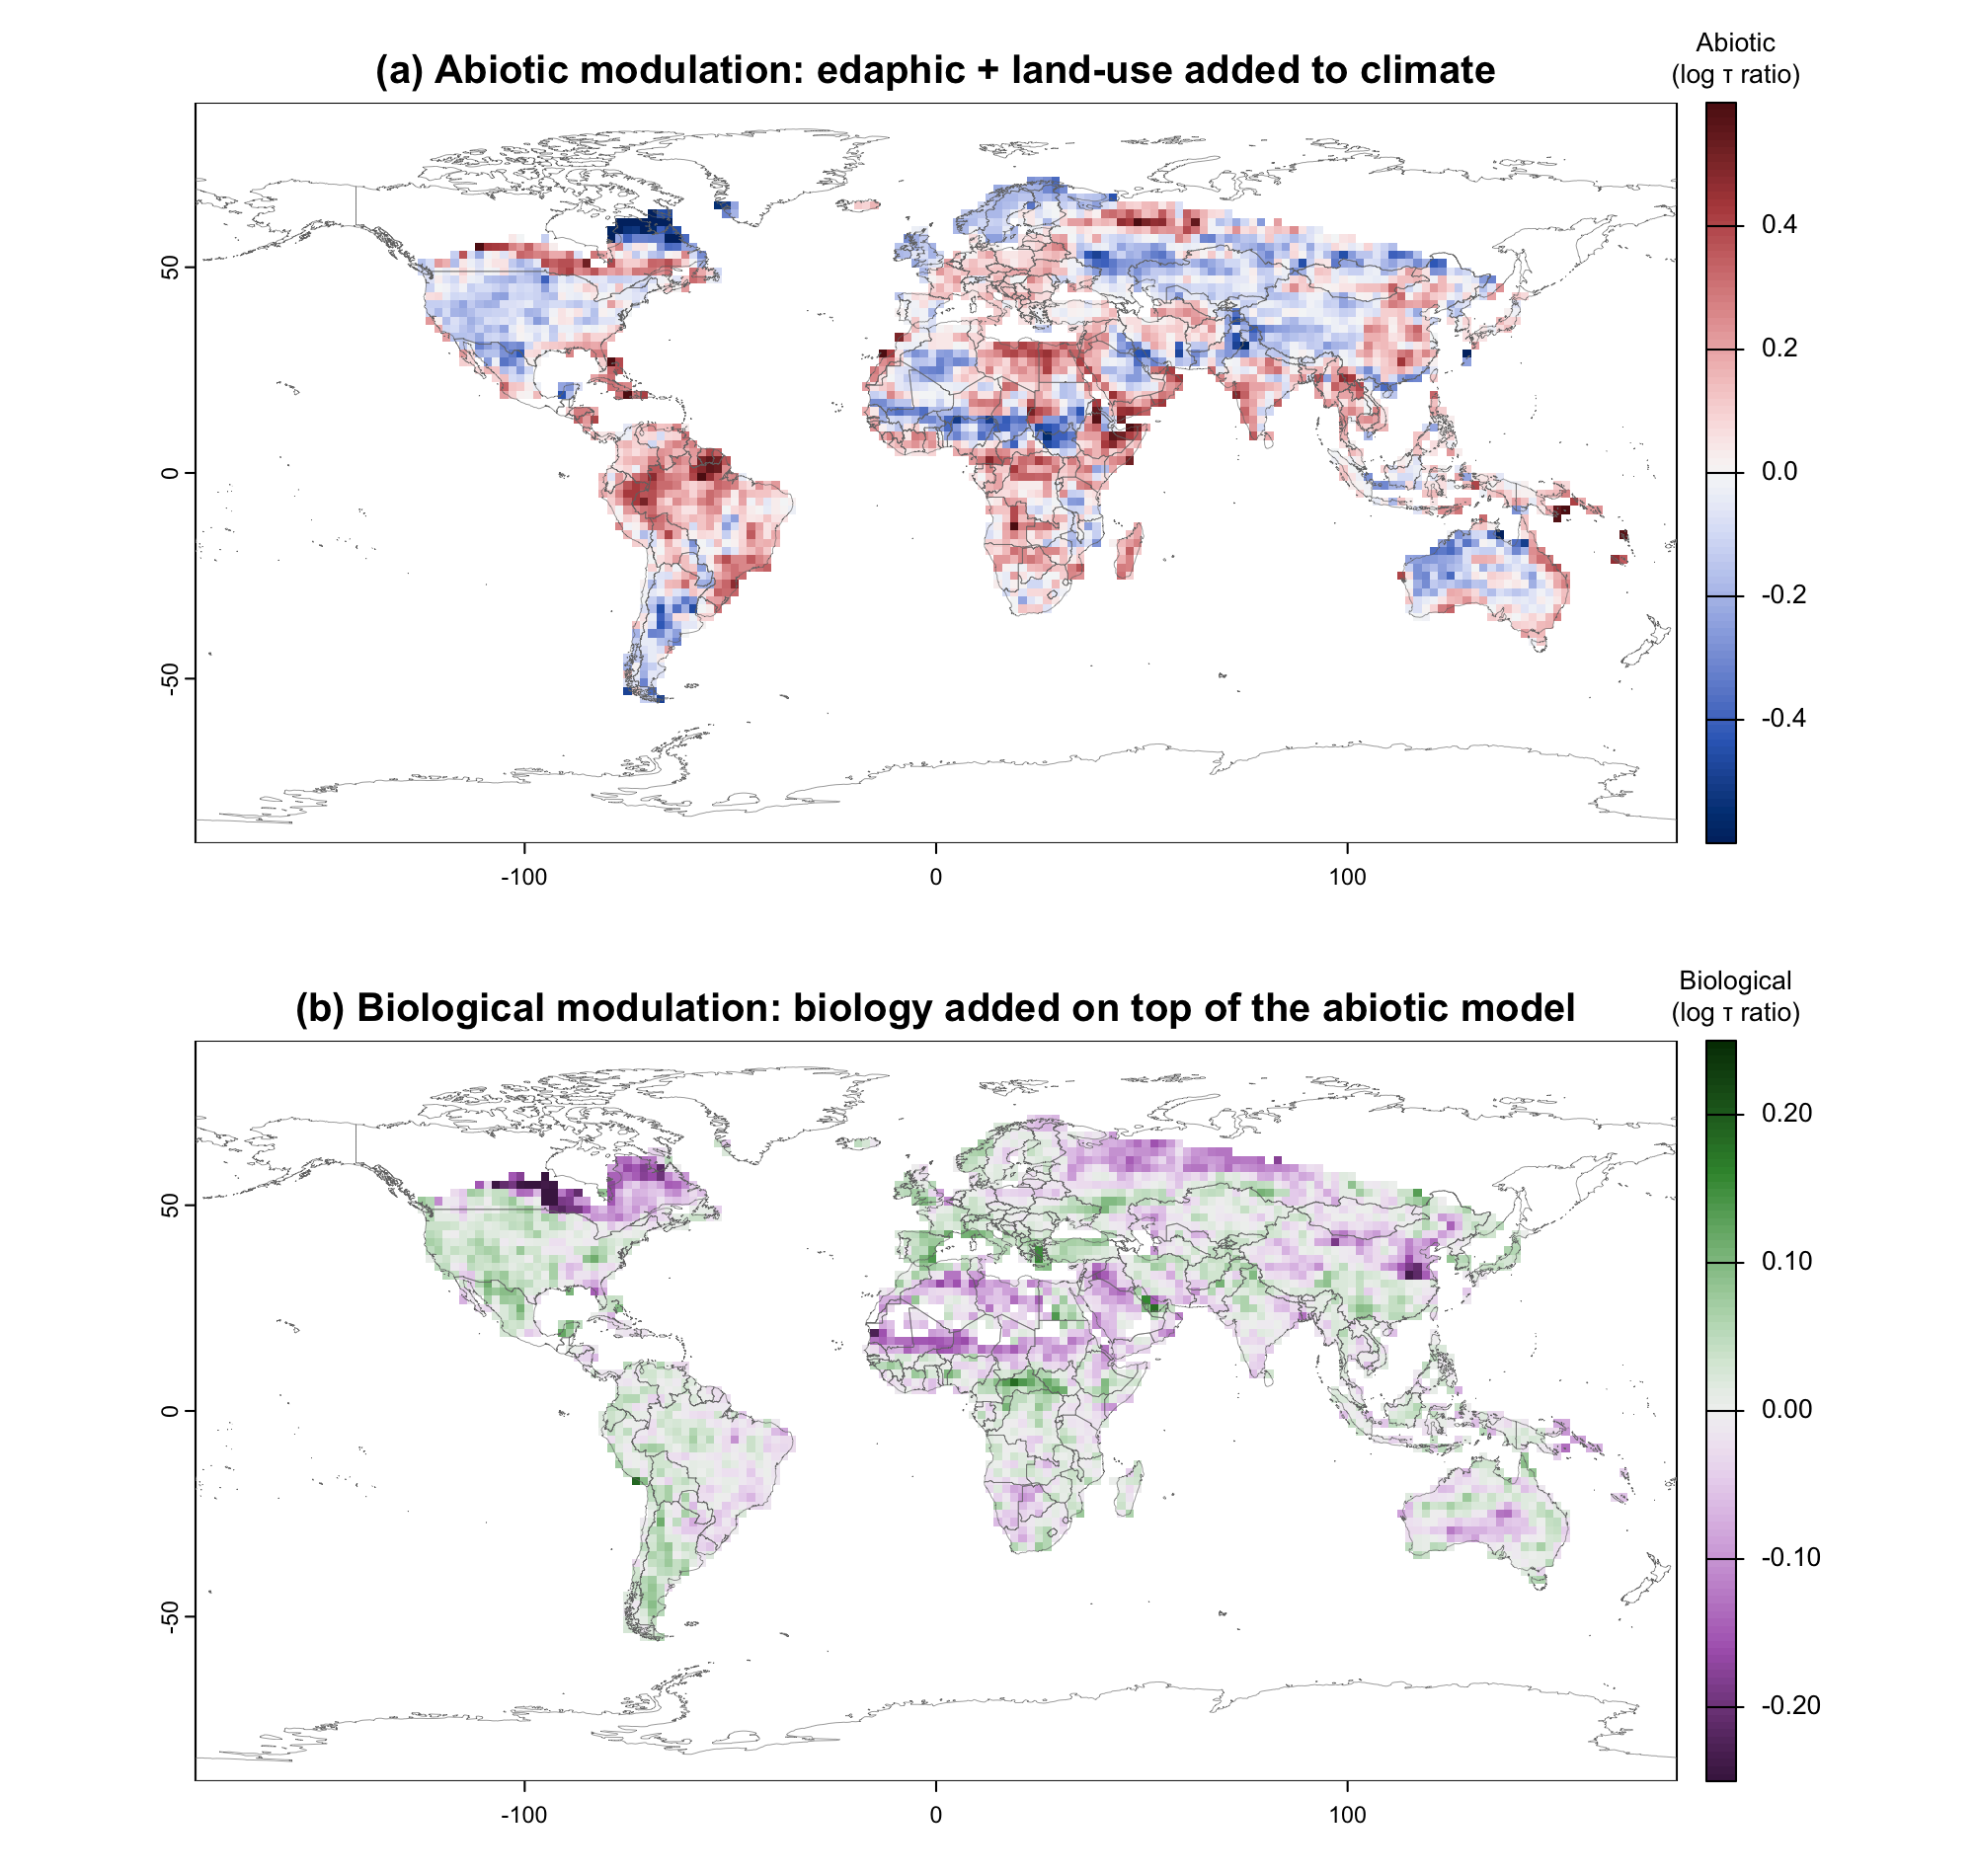
\includegraphics[width=0.8\textwidth]{../plots/step_15b_zonality/zonality_map_dual.png}
\caption{\textbf{Zonality map (nested).} As Fig.~\ref{fig:zonality}, but the two domains are taken sequentially rather than symmetrically: (a)~abiotic modulation relative to climate and (b)~biological modulation added on top of the abiotic model (order-dependent), at meso (2\textdegree) scale. Red/green~=~longer turnover, blue/purple~=~shorter.}
\label{fig:nestedmap}
\end{figure}
% Former appendix figure "Dominant beyond-climate modulator" (fig:zonality_dominant)
% promoted 2026-07-09 into the main-text zonality figure as panel (c); see fig:zonality.

\begin{figure}[H]\centering
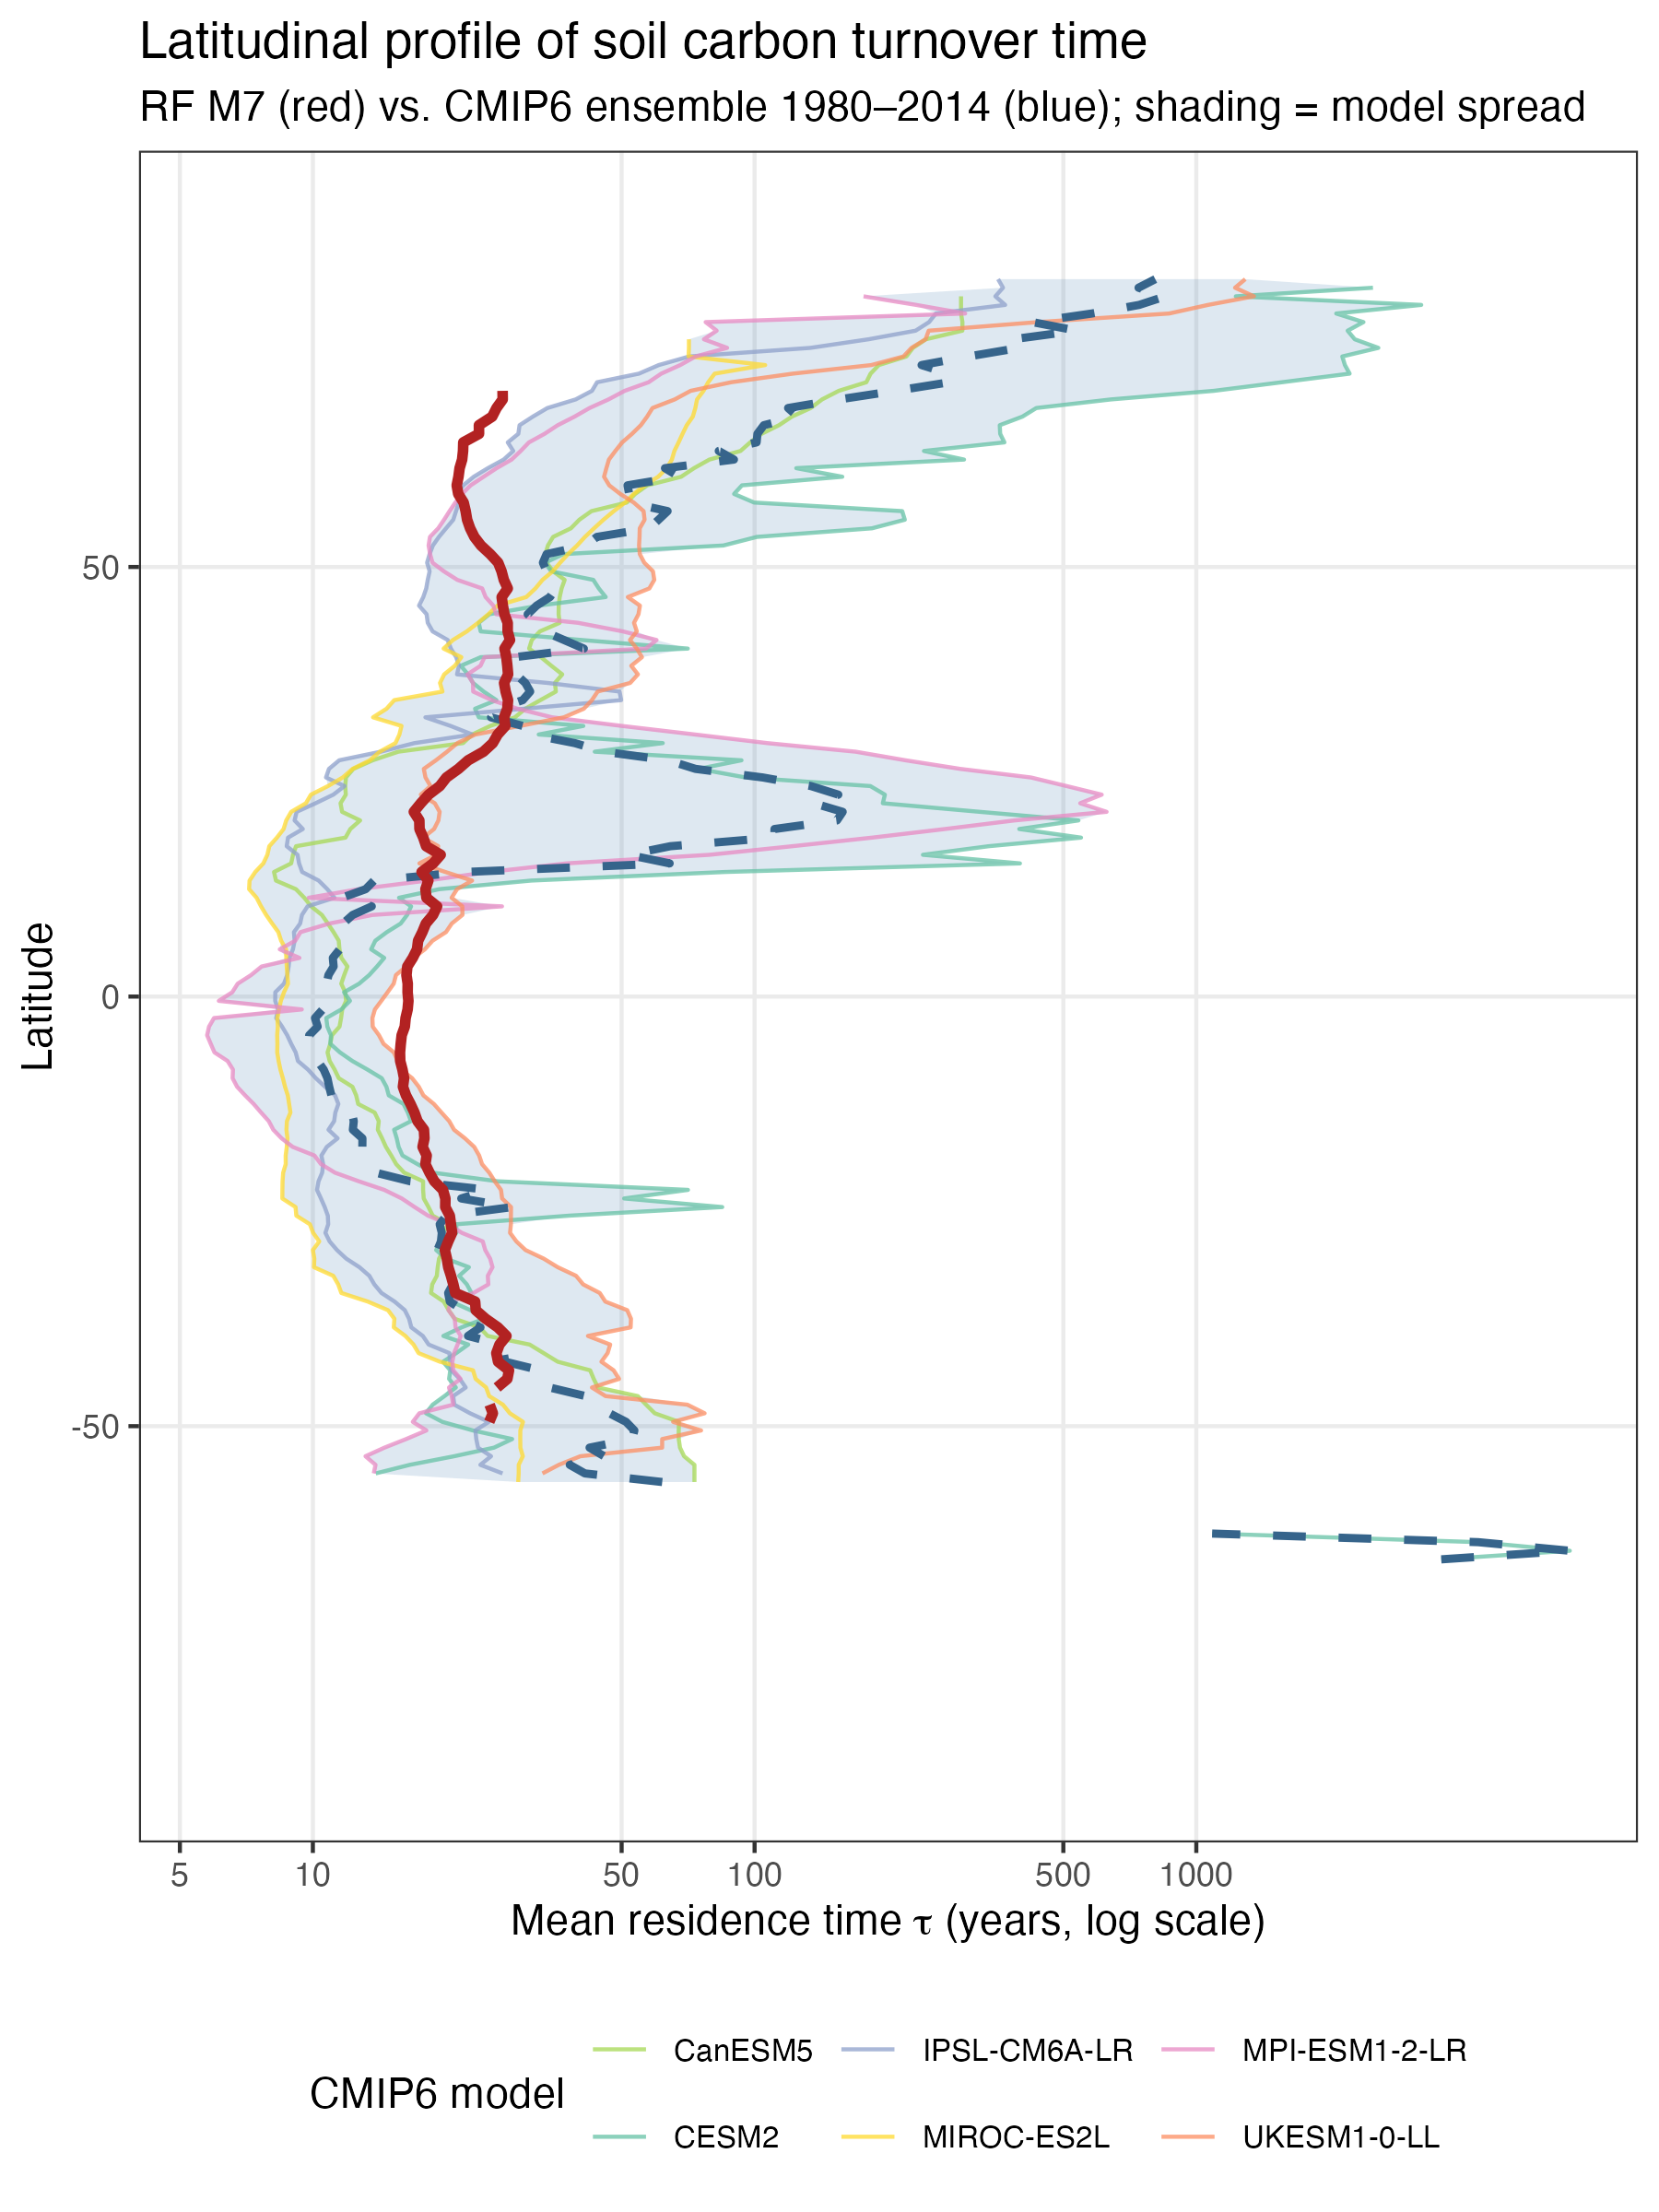
\includegraphics[width=0.7\textwidth]{../plots/step_20/fig_latitudinal_profile.png}
\caption{\textbf{Absolute latitudinal profile} of $\tau$ (log axis): CMIP6 members, ensemble mean, and RF~M7 (the magnitude counterpart, resolved in-text via the normalised comparison).}
\label{fig:esm_profile}
\end{figure}

\begin{figure}[H]\centering
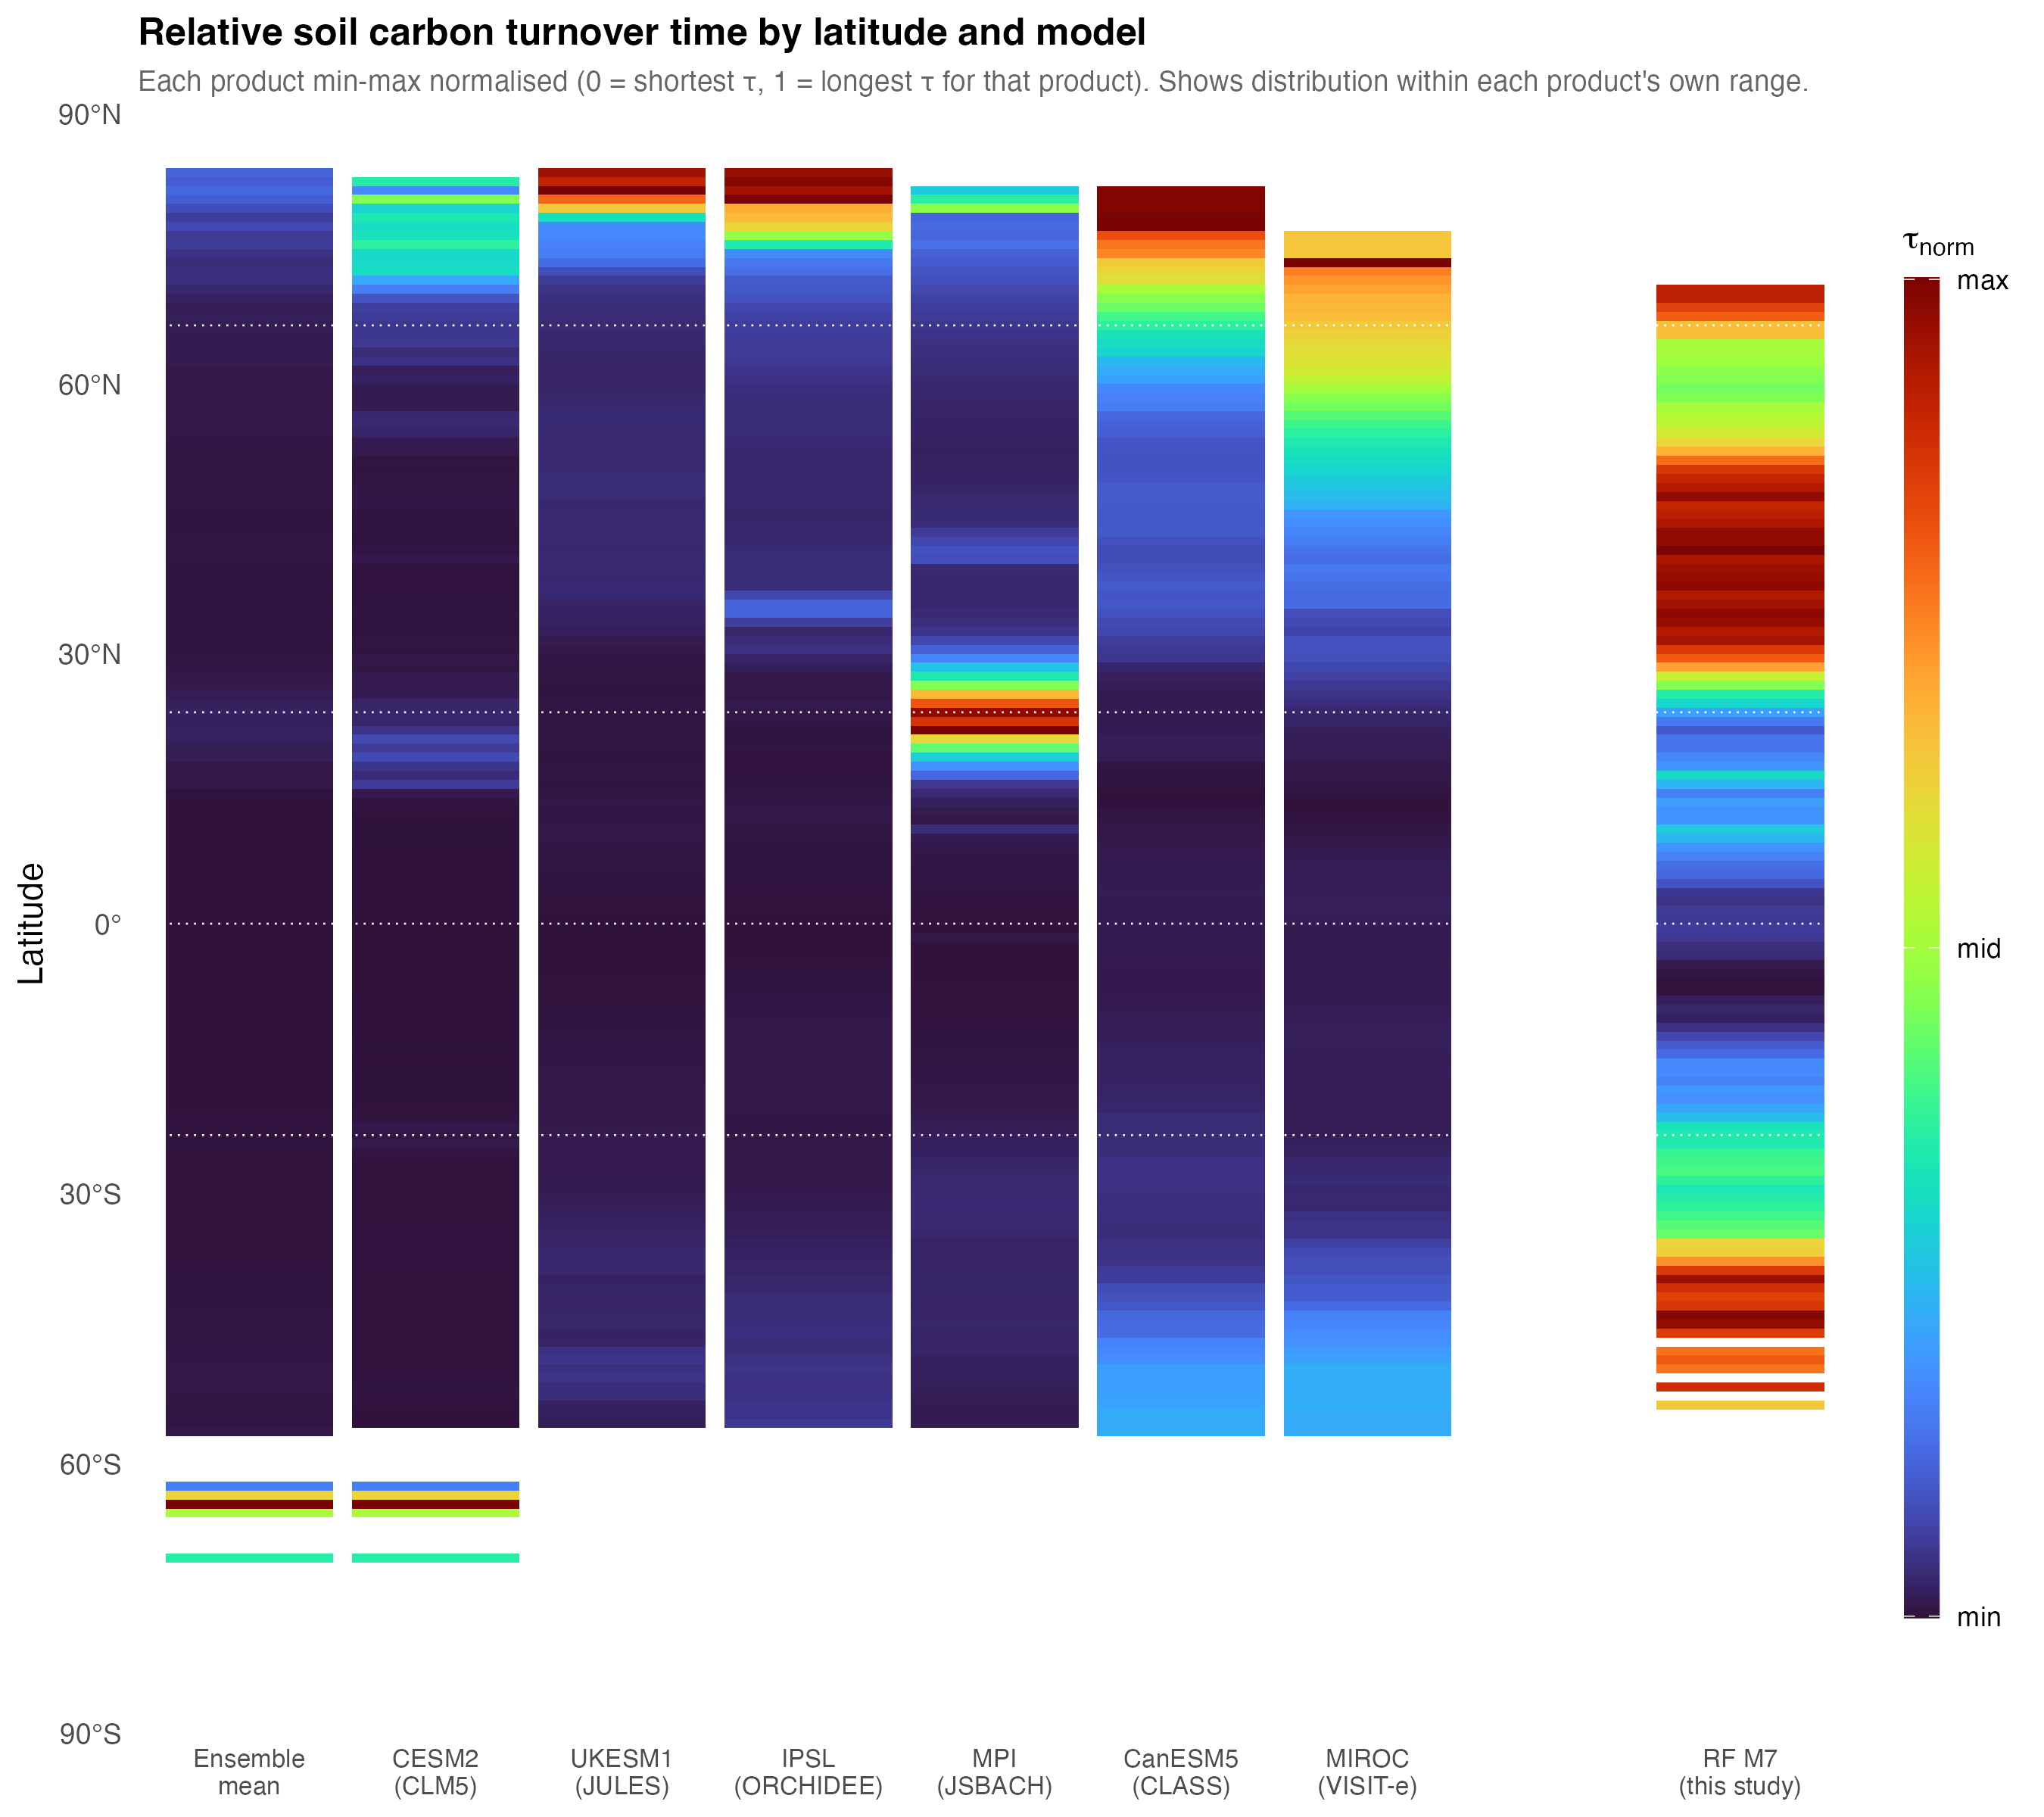
\includegraphics[width=0.92\textwidth]{../plots/step_20/fig_latitude_heatmap_relative.png}
\caption{\textbf{Relative latitudinal structure} of $\tau$ across the CMIP6 ensemble and the estimate of this study; each column min--max normalised (continuous-latitude companion to the biome figure).}
\label{fig:esm_heatmap}
\end{figure}



\subsection*{Provenance control on the beyond-climate signal}

% numbers below are from the 300-tree validation run and are expected to be stable.
Because the soil compendium aggregates 44~source databases that are
geographically clustered, a source-specific measurement or laboratory offset
could in principle masquerade as large-scale (zonal) structure. We therefore
tested whether the beyond-climate signal (the residual of the spatial-block
cross-validated climate model) is carried by data provenance rather than
ecology. Only \textbf{2.4\,\%} of the residual variance lies between source
databases ($\eta^2_\text{source}=0.024$, versus $\eta^2=0.067$ for
5\textdegree{} spatial blocks). Removing each source's mean residual leaves the
coarse-scale organisation essentially intact and the covariate skill on the
block-mean (zonal) residual barely changed (Table~\ref{tab:provenance}); the
mid-range semivariogram structure is likewise unaffected. Because source
membership is itself confounded with geography, this is a conservative
(upper-bound) test: the signal that survives source removal is unambiguously
ecological. We conclude that the modest zonal organisation of soil carbon
turnover is a real ecological pattern, not an artefact of data compilation.

\begin{table}[h!]
  \centering
  \small
  \caption{%
    \textbf{Provenance control.} Coarse-scale organisation of the
    beyond-climate residual (ratio of observed between-block variance to the
    spatial-randomness null) and covariate skill on the block-mean residual,
    before and after removing each source database's mean. The signal is
    essentially unchanged, indicating it is ecological rather than a
    source/laboratory artefact.}
  \label{tab:provenance}
  \begin{tabular}{lcc}
    \toprule
    Metric & Before & After source de-meaning \\
    \midrule
    Between-source variance share ($\eta^2_\text{source}$) & \multicolumn{2}{c}{0.024 (2.4\,\%)} \\
    Organisation @\,2\textdegree{} (obs/null)   & $5.3\times$  & $5.1\times$ \\
    Organisation @\,5\textdegree{} (obs/null)   & $7.2\times$  & $6.4\times$ \\
    Organisation @\,10\textdegree{} (obs/null)  & $11.6\times$ & $10.1\times$ \\
    Block-mean covariate $R^2$ @\,5\textdegree{} & 0.188 & 0.152 \\
    \bottomrule
  \end{tabular}
\end{table}


\subsection*{Appendix tables}

\begin{table}[h!]
  \centering
  \small
  \caption{%
    \textbf{Belowground NPP allocation fractions ($f_\text{BNPP}$) by
    dominant land cover class used to estimate soil carbon input.}
  }
  \label{tab:allocation}
  \begin{tabular}{lcc}
    \toprule
    Land cover class & ESA code & $f_\text{BNPP}$ \\
    \midrule
    Tree cover            & 10  & 0.35 \\
    Shrubland             & 20  & 0.45 \\
    Grassland             & 30  & 0.55 \\
    Cropland              & 40  & 0.30 \\
    Built-up              & 50  & 0.20 \\
    Bare/sparse           & 60  & 0.30 \\
    Herbaceous wetland    & 90  & 0.50 \\
    Mangroves             & 95  & 0.40 \\
    Moss/lichen           & 100 & 0.60 \\
    \midrule
    \textit{Default (missing)}  & --- & 0.40 \\
    \bottomrule
  \end{tabular}
\end{table}

\begin{table}[h!]
\centering
\small
\caption{Carbon-input sensitivity of the beyond-climate signal. The soil carbon input coefficient is re-derived on the same NPP field under three conventions (belowground, total NPP, and total minus a generous forest-harvest export $h$). Block-CV $R^2$, the beyond-climate gap (full $-$ climate-only), Moran's $I$ of the beyond-climate residual, and the four Shapley shares are all but unchanged; only LandUse responds, as expected for a land-cover-structured coefficient.}
\label{tab:input_sensitivity}
\begin{tabular}{lrccccrrrr}
\toprule
 & & \multicolumn{2}{c}{Block-CV $R^2$} & Gap & Moran's & \multicolumn{4}{c}{Shapley share (\%)} \\
\cmidrule(lr){3-4}\cmidrule(lr){7-10}
Convention & $n$ & full & clim. & (pp) & $I$ & C & E & B & L \\
\midrule
Belowground (main) & 150,863 & 0.390 & 0.319 & 7.1 & 0.253 & 35.4 & 32.7 & 22.2 & 9.6 \\
Total NPP & 148,714 & 0.389 & 0.319 & 6.9 & 0.260 & 36.3 & 31.6 & 21.5 & 10.6 \\
Total $-$ harvest ($h{=}0.5$) & 149,207 & 0.390 & 0.302 & 8.8 & 0.256 & 34.0 & 32.9 & 21.6 & 11.4 \\
\bottomrule
\end{tabular}
\end{table}

\begin{table}[h!]
  \centering
  \small
  \caption{%
    \textbf{Magnitude-free measures of spatial dispersion in $\tau$
    across products.}
    Computed over all valid land pixels on the common 1\textdegree{}
    grid for each product. CV~=~coefficient of variation (SD/mean);
    $\tau_{95}/\tau_{5}$~=~ratio of 95th to 5th percentile;
    SD$_{\ln \tau}$~=~standard deviation of natural-log-transformed $\tau$,
    the dispersion measure most insensitive to extreme tails.
  }
  \label{tab:esm_dispersion}
  \begin{tabular}{llcccc}
    \toprule
    Product & LSM & Mean $\tau$ (yr) & CV & $\tau_{95}/\tau_{5}$ &
    SD$_{\ln \tau}$ \\
    \midrule
    CESM2          & CLM5         & 193.8 & 3.64 & 112.0 & 1.38 \\
    UKESM1-0-LL    & JULES        &  63.3 & 3.09 &  10.0 & 0.82 \\
    IPSL-CM6A-LR   & ORCHIDEE     &  27.5 & 2.02 &   6.3 & 0.74 \\
    MPI-ESM1-2-LR  & JSBACH       &  62.8 & 3.48 &  40.2 & 1.10 \\
    CanESM5        & CLASS-CTEM   &  48.6 & 1.32 &  26.1 & 1.05 \\
    MIROC-ES2L     & VISIT-e      &  31.4 & 0.90 &  10.7 & 0.89 \\
    \midrule
    CMIP6 ensemble & ---          & \multicolumn{4}{c}{--- (see individual models)} \\
    RF~M7 (this study) & ---      &  23.2 & 0.39 &   3.7 & 0.42 \\
    \bottomrule
  \end{tabular}
\end{table}

\end{document}